\section{Heur\'istica de B\'usqueda Local} \label{ej4}
Un algoritmo de Búsqueda Local consiste de dos pasos: elegir una solución inicial y luego, visitar soluciones parecidas hasta encontrar la mejor posible.\\

Para cada solución factible s $\epsilon$ S se define N(s) como el conjunto de
``soluciones vecinas'' de s. Un procedimiento de busqueda local toma una solución inicial s e iterativamente la mejora reemplazándola por otra solución mejor del conjunto N(s), hasta llegar a un óptimo local.\\

Sea s $\epsilon$ S una solución inicial\\
 
Mientras exista s' $\epsilon$ N(s) con f(s) $>$ f(s')\\
 
s $\leftarrow$ s'\\

Donde $f: s \rightarrow \mathbb{N}$ es una funci\'on que mapea soluciones factibles del problema a Naturales. Nuestra funci\'on devuelve el cardinal de s.\\

Nuestro objetivo es minimizar $f$, por lo tanto nuestras vecindades planteadas son de la forma, $f(s) - 1 == f(s')$ o bien $f(s) - 2 == f(s')$, es decir que cada conjunto de N(s) tiene cardinal $s - 1$ o bien $s - 2$.

\subsection{Explicaci\'on}
%Explicar detalladamente el algoritmo implementado. Plantear al menos dos vecindades distintas para la busqueda y al menos dos soluciones iniciales.

Considerando el problema a tratar, establecimos nuestros criterios para encontrar las soluciones iniciales y las vecindades.


\subsubsection{Elección de Solución Inicial}

Al momento de seleccionar la solución Inicial, determinamos dos criterios.

\subsubsection*{Criterio I Solución Inicial: Golosa}

Se realiza una ejecución del algoritmo Goloso de la Sección \ref{ej3}.\\

Esto quiere decir, se ordenan los nodos por grado de manera decreciente. Se eligen los nodos de a uno (de mayor a menor), de modo que al elegir un nodo se descartan sus vecinos para sus futuras elecciones.

\subsubsection*{Criterio II Solución Inicial: Secuencial}

Los nodos al ser ingresados como parámetro del algoritmo tienen como identificador un número entre $0$ y $n-1$. El orden que vamos a utilizar para recorrerlos es el que haya sido dado cuando fueron ingresados como parámetro.\\

Lo primero que realizamos es tomar al nodo $0$ y considerarlo parte de la solución. Se descartan todos los nodos vecinos a él y se continúa el proceso con el nodo que tenga menor número de \textit{id}.

De este modo se forma un conjunto solución tal que en cada paso añade al nodo disponible que tenga su identificador número menor.

\subsubsection{Elección de Vecindad}

Dada una soluci\'on al problema, se establece un conjunto de soluciones ``similares'' denominadas \emph{vecinas}. Los criterios para elegir esta vecindad pueden variar.

\subsubsection*{Criterio I Vecindad}

El primer criterio elegido es, a partir de una soluci\'on, quitarle dos nodos y agregarle uno que no haya sido contenido.\\

Para ello, se prueban todas las combinaciones de pares de nodos dentro del conjunto posibles y se considera a los nodos que tienen ambas como vecinos. Si al sacar este par y agregar el nuevo nodo, se obtiene un conjunto Independiente Dominante M\'inimo, se actualiza el conjunto soluci\'on. 

\subsubsection*{Criterio II Vecindad}

El segundo criterio es similar al anterior, s\'olo que ahora consideramos quitar tres nodos y agregar uno.\\

Se consideran todas las combinaciones posibles de grupos de tres nodos dentro del conjunto soluci\'on inicial y se prueba con los nodos que sean vecinos de todos ellos si forman un conjunto soluci\'on.\\

\newpage
\subsection{Complejidad Temporal}
%Calcular el orden de complejidad temporal de peor caso de una iteracion del algoritmo de busqueda local (para las vecindades planteadas). Si es posible, dar una cota superior para la cantidad de iteraciones de la heurıstica.
Este algoritmo llama, seg\'un la vecindad a ejecutar, a una de las siguiente dos funciones, que dominan la complejidad del ciclo.

\subsubsection{dameParesVecinosComun}\label{vec1}

Funciones usadas:\\
listaAd::dameVecinos\\
push_back\\
size\\

Dado un conjunto de nodos, se buscan todas las combinaciones de pares de nodos posibles. 
Luego, para cada par de nodos (i,j) se recorren: la lista de adyacencia de i y la de j. 
Por cada elemento que pertenezca a las dos listas, se a\~nade al vector \texttt{vecinosEnComun} dentro de la estructura pares.

\begin{algorithm}[h!]
struct vecinosEnComun\{\\
	unsigned int nodoA;\\	
	unsigned int nodoB;\\
	vector$<$unsigned int$>$ vecinosComun;\\
\};
\end{algorithm}

\begin{algorithm}[h!]
	\For{int i = 0; i $<$ optimo.size(); ++i}{
		\For{int j = i+1; j $<$ optimo.size(); ++j}{
			list$<$unsigned int$>$* vecinosA = adyacencia.dameVecinos(optimo[i]);\\
			list$<$unsigned int$>$* vecinosB = adyacencia.dameVecinos(optimo[j]);\\
			vecinosEnComun par;\\
			par.nodoA = optimo[i];\\
			par.nodoB = optimo[j];\\
			list$<$unsigned int$>$::iterator itVecinosA = vecinosA-$>$begin(), itVecinosB = vecinosB-$>$begin();\\
			\While{itVecinosA != vecinosA-$>$end() and itVecinosB != vecinosB-$>$end()}{
				\eIf{*itVecinosA == *itVecinosB}{
					par.vecinosComun.push_back(*itVecinosA);\\
					itVecinosA++;\\
					itVecinosB++;\\
				}{
					\eIf{*itVecinosA $>$ *itVecinosB}{
						itVecinosB++;
					}{
						itVecinosA++;
					}
				}
			}
			\If{par.vecinosComun.size() $>$ 0}{
				pares.push_back(par);
			}
		}
	}
\end{algorithm}

Para elegir todos los pares posibles de nodos en el conjunto \texttt{\'optimo}, se recorre mediante dos \emph{for}s.\\
El primero itera i desde 0 hasta el \'ultimo elemento y el segundo desde i hasta el \'ultimo elemento.\\
De este modo, cada par de nodos se recorre una \'unica vez. Ya que es lo mismo el par (i,j) que (j,i).\\

Dentro de los \emph{for}s anidados, se crea una estructura \texttt{vecinosEnComun} \textbf{par} donde el nodoA es i y el nodoB es j.\\

Para poder armar la lista vecinosComun (miembro de la estructura vecinosEnComun), se iteran las listas de adyacencia con itVecinosA (i) e itVecinosB (j).\\

Como ambas listas fueron ordenadas antes de invocar a la funci\'on dameParesVecinosComun, es posible encontrar elementos en com\'un recorriendolas secuencialmente de manera simult\'anea.\\

Se procede de manera simple, si nodo(itVecinosA) es igual a nodo(itVecinosB) entonces se a\~nade el nodo actual a la lista vecinosComun.\\

En caso contrario, se avanza el iterador que sea menor.\\

Si conclu\'ida la iteraci\'on de las dos listas de adyacencia, la lista vecinosEnComun posee al menos un elemento; entonces se agrega \textbf{par} a la soluci\'on.

Dado un par (i,j), la complejidad de recorrer ambas listas de adyacencia es de: $O(grado(i)+grado(j))$.
Cada par se recorre una \'unica vez. Por lo tanto, los dos \emph{for}s anidados van a iterar (considerando a (n-1) como el \'ultimo nodo'):\\

Cuando sea el par de nodos (0,1) : grado(0)+grado(1) \\

Cuando sea el par de nodos (0,2) : grado(0)+grado(2) \\

...\\

Cuando sea el par de nodos (0,n-1) : grado(0)+grado(n-1)\\

Cuando sea el par de nodos (1,2) : grado(1)+grado(2)\\

Cuando sea el par de nodos (1,3) : grado(1)+grado(3)\\

...\\

Cuando sea el par de nodos (1,n-1) : grado(1)+grado(n-1)\\

...\\

Cuando sea el par de nodos (n-2,n-1) : grado(n-2)+grado(n-1)\\


Se puede apreciar que el grado de cada nodo se suma (n-1) veces. Por lo tanto, al sumar las complejidades da un total de:\\

grado(0)*(n-1) + grado(1)*(n-1) + ... + grado(n-1)*(n-1)\\

lo que es equivalente a:\\

[grado(0)+grado(1)+ ... + grado(n-1)]*(n-1)\\

La complejidad en peor caso se obtiene cuando los grados de todos los nodos son maximos, por lo tanto se trata de un grafo completo.
Donde vale que 2*\#ejes = grado(0)+grado(1)+ ... grado(n-1).\\

Por consecuencia, la complejidad de esta funci\'on es de:\\

O(2*\#ejes*(n-1)) lo que equivale a O(\#ejes*n) que pertenece a O($n^3$) ya que la mayor cantidad de ejes que puede tener un grafo es ((n-1)n)/2


\subsubsection{dameTernasVecinasComun}\label{vec2}

La funci\'on dameTernasVecinasComun funciona de manera an\'aloga a la descripta en el inciso \ref{vec1}.\\

Se va a encargar de armar tomar de todas las maneras posibles tres nodos del conjunto pasado por par\'ametro.\\

Luego, obtener los nodos (si existe) que sean vecinos de los tres.\\

De esta manera, recorre el conjunto con tres \emph{for}s tal que cada tupla la recorre una sola vez.\\

En este caso el c\'alculo de cada iteraci\'on, dada la tupla (i,j,k), ser\'a de grado(i)+grado(j)+grado(k).\\

Dada la tupla (0,1,2) el costo ser\'a: grado(0)+grado(1)+grado(2)\\

Dada la tupla (0,1,3) el costo ser\'a: grado(0)+grado(1)+grado(3)\\

...\\

Dada la tupla (0,1,n-1) el costo ser\'a: grado(0)+grado(1)+grado(n-1)\\

Dada la tupla (0,2,3) el costo ser\'a: grado(0)+grado(2)+grado(3)\\

...\\

Dada la tupla (0,n-2,n-1) el costo ser\'a: grado(0)+grado(n-1)+grado(n-2)\\

Dada la tupla (1,2,3) el costo ser\'a: grado(1)+grado(2)+grado(3)\\

...\\

Dada la tupla (n-3,n-2,n-1) el costo ser\'a: grado(n-3)+grado(n-2)+grado(n-1)\\

En el peor caso, el grado de todos los nodos es de n (grafo completo). Por lo tanto, el costo de cada iteraci\'on es de O(3n).\\

La cantidad de ternas que se pueden formar es de $(n(n-1)(n-2))/6$, equivale a decir que va a iterar $O(n^3)$ veces con costo $O(3n)$ cada vez.\\

Dando una complejidad de $O(n^4)$.

\newpage
\subsubsection{localCIDM}

\begin{algorithm}[h!]
optimo = genero_instancia_inicial();\\
\eIf{cae_en_optimizacion(optimo)}{
	return optimizacion(optimo);
	}{
	optimo.sort();\\
	\While{hay cambios posibles}{
		vector$<$vecinosEnComun$>$ vecinos = encontrar_vecinos_en_comun(optimo);\\
		\eIf{no hay vecinos}{
			salir del ciclo
			}{
			\While{hay vecinos}{
				eliminar par o terna con vecino en comun;\\
				\For{cada vecino en comun}{
					lo agrego al optimo;\\
					veo si es CID;\\
					\If{no lo es}{
						restauro y miro el siguiente vecino;
					}
				}
			}
			\eIf{es CID}{
				lo asigno al optimo;\\
				vuelvo al ciclo principal;
			}{
				restauro optimo;\\
				veo la siguiente tupla o termino;
			}
		}
	}
}
\end{algorithm}

Como primera medida, ordena todas las listas de adyacencia: listaAd::ordenar, esto toma $O(n^2.log(n))$, para cada nodo ($n$) ordenar su lista de adyacencia (en el caso del grafo completo, tendr\'an ($n-1$) vecinos, y ordenarlos toma $O(n.log(n))$)\\

Para las \textbf{ejecuciones 3 y 5}, el parametro greedy esta en true, por lo tanto comienza con una solucion inicial golosa. Por lo tanto invoca a la funcion greedyCIDM() la cual tiene complejidad $O(n^2)$ explicada en el inciso \ref{ej3}.\\

\bigskip

Para las \textbf{ejecuciones 2 y 4}, la solucion inicial es secuencial. Esto quiere decir que para obtener una primera soluci\'on al problema se arma un vector \texttt{nodos} con la cantidad de nodos, donde en la posici\'on i se encuentra el nodo i.\\

Se recorre secuencialmente este arreglo (desde la posici\'on cero) de modo que se a\~nade el nodo actual a la soluci\'on y se elimina del vector \texttt{nodos}.\\

Luego, se borran tambi\'en del vector a los vecinos del nodo actual.\\

En la siguiente iteraci\'on se tienen $n-1-(grado(0))$ elementos en el vector \texttt{nodos}.\\

Lo cual, en el peor caso, ser\'ia n-1 donde grado(0)=0.\\

Considero la notaci\'on vecinos(i) como la cantidad de nodos pertenecientes al vector \texttt{nodos} durante la iteraci\'on i que sean adyacentes al nodo i.\\

En la iteraci\'on i, el vector va a contener $n-1-grado(0)- ... -1-vecinos(i)$\\

Donde en el peor caso, tambi\'en, deber\'a ser vecinos(i) con valor m\'inimo. Por consecuente, el peor caso es un grafo donde cada nodo es una componente conexa trivial, es decir que no existen ejes.\\
	
En el peor caso, itera n veces ya que el tama\~no del vector disminuye s\'olo en una unidad por iteraci\'on.\\

El costo de las operaciones por iteraci\'on es $O(n)$.\\

Las funciones usadas son:\\

push_back (costo $O(n)$ amortizado)\\

listaAdy::sonVecinos (costo $O(min(grado(nodoA), grado(nodoB)))$)\\

Por lo tanto esta seccion es del orden de O($n^2$)

\bigskip

A continuaci\'on, se introducen optimizaciones del algoritmo.

\begin{itemize}
\item En primer lugar, si la soluci\'on \'optima actual posee tama\~no 1 no va a encontrarse una soluci\'on mejor, por consiguiente se devuelve. (Costo $O(1)$)
\item En segundo lugar, si la soluci\'on \'optima actual posee tama\~no 2 la \'unica soluci\'on que puede ser mejor es la que posee un s\'olo nodo. Se chequea si existe una soluci\'on con un s\'olo nodo (costo $O(n)$). Si existe, la soluci\'on \'optima es la de un s\'olo nodo y se devuelve sino era la soluci\'on con dos nodos. Funciones usadas: assign, listaAdy::gradoDeNodo y listaAdy::cantNodos (todas con costo $O(1)$)
\item En tercer lugar, si la soluci\'on \'optima actual posee tama\~no n debe ser la soluci\'on que se retorne. Ya que la \'unica manera de que todos los nodos sean parte del conjunto soluci\'on al problema es que cada uno sea una componente conexa, es decir no existan ejes. A continuaci\'on, debe ser la soluci\'on devuelta. (Costo $O(1)$)
\end{itemize}

Si la ejecuci\'on del algoritmo no entr\'o en ninguno de los casos citados, se prosigue ordenando al vector de soluci\'on \'optima. (Costo $O(n.log(n))$, en el peor caso tiene $n-1$ elementos)\\

Ahora se prosigue con las iteraciones por vecindades.\\

En los casos de \textbf{ejecuci\'on 2 y 3}, se pasa por par\'ametro el valor de vecindad==true. Se ejecuta la funci\'on dameParesVecinosComun (vista en \ref{vec1}), es decir por cada iteraci\'on se querr\'a tomar un par de nodos tal que sea posible quitarlos y agregar un vecino de ambos al conjunto soluci\'on y se obtenga una soluci\'on con un nodo menos.\\

Se iterar\'a en un while hasta que la variable hayCambiosHechas sea false (complejidad $O(n)$ explicada m\'as adelante).\\

Lo primero que se hace es ejecutar \texttt{dameParesVecinosComun()} (complejidad $O(n^3)$).\\

Si esta funci\'on no devolvi\'o ning\'un par, se debe salir del ciclo.\\

Se ejecuta otro while, mientras haya pares sin ser visitados (de los obtenidos) (complejidad $O(n.(n-1)/2) = O(n^2)$).\\

Como lo que se quiere hacer es borrar nodos del conjunto soluci\'on, se hace en una copia porque a priori no se sabe si conducir\'a a un conjunto que sea soluci\'on.\\

Se borra del conjunto soluci\'on al par actual (i,j) que por el modo en que armamos los pares siempre se cumple que $i<j$. Esto tiene un costo de O(n) ya que itera la soluci\'on hasta que encuentre j y en el medio elimina i. Se borra con el operador \texttt{erase} de iterador (complejidad $O(3n) en el peor caso$).\\

Ahora resta ver si al agregar alg\'un nodo en com\'un se forma un conjunto soluci\'on que sea Independiente Maximal. Recorreremos la lista de nodos que tienen en com\'un i y j para ver si al agregar alguno de ellos al conjunto soluci\'on, el conjunto obtenido cumple ser Independiente Dominante M\'inimo. Es decir, se itera la lista de vecinos hasta encontrar un nodo que al insertarlo cumpla ser un conjunto soluci\'on v\'alido o hasta que termine sin haber podido formar un CIDM.\\

Lo que tendr\'a un costo de $O(n^2)$.\\

Primero se fija que esta combinaci\'on de quitar los nodos (i,j) y agregar el nodo actual no se haya probado todav\'ia, si es as\'i se agrega el nodo actual de la lista al conjunto soluci\'on de manera ordenada. Se itera el vector hasta la posici\'on donde se debe insertar lo que tiene costo de O(n) ya que en peor caso en la soluci\'on original hab\'ia n-1, se sacaron i y j por lo que el vector qued\'o de un tama\~	no n-2. Si el nodo a insertar debe hacerse al final, recorre todos.\\

iterator::insert tiene complejidad $O(n)$\\

Ahora con el conjunto formado se invoca a la funci\'on lisAdy::esIndependienteMaximal que tiene una complejidad de $O(n^2)$\\

Si el conjunto armado hasta el momento no es Independiente Maximal, vamos a querer borrar el nodo a\~nadido \'ultimo por lo que se itera de nuevo el vector hasta encontrarlo y borrarlo con iterator::erase con un costo total de O(n).\\

Este c\'odigo si al momento de quitar dos nodos (i,j) puede a\~nadir diversos nodos y con cualquiera resulta un conjunto Independiente Maximal, s\'olo considera al primero que logre cumplir ser un conjunto Independiente Maximal.\\

Si al quitar dos nodos y agregar uno se logr\'o un conjunto soluci\'on v\'alido se actualiza el vecotr soluci\'on \texttt{optimo}.\\

El ciclo mayor iterar\'a hasta que no se hagan m\'as cambios. Esto va a pasar cuando haya probado todos los pares de nodos posibles y por cada uno probado a\~nadir otro.\\

Es decir, en el peor caso se comenz\'o con una soluci\'on inicial de n-1 nodos y, se quitaron dos y a\~nadi\'o uno hasta que la soluci\'on final quede de tama\~no 1. Es decir, el while m\'as grande iterar\'a en peor caso n veces.\\

Por cada par de nodos iterar\'a $n^2$ veces y la cantidad de pares posibles en peor caso ser\'a de $O(n^2)$.\\

Por lo tanto el costo de cada iteraci\'on del ciclo mayor ser\'a de $O(n^4)$, iter\'andola n veces dar\'a un costo total del algoritmo de $O(n^5)$.\\

\bigskip	

En los casos de \textbf{ejecuci\'on 4 y 5}, el procedimiento ser\'a similar.\\

Primero buscar\'a ternas con vecinos en com\'un (\texttt{dameTernasVecinasComun}) con un costo de $O(n^4)$.\\

Pero el costo de cada iteraci\'on del ciclo mayor ser\'a de $O(n^4)$, por lo explicado anteriormente, con lo cual el costo total del algortimo es $O(n^5)$ tambi\'en para esta vecindad. 


\newpage
\subsection{Experimentaci\'on}
%Realizar una experimentacion que permita observar la performance del algoritmo comparando los tiempos de ejecucion y la calidad de las soluciones obtenidas, en funcion de las vecindades y las soluciones iniciales utilizadas y elegir, si es posible, la configuracion que mejores resultados provea para el grupo de instancias utilizado.

El objetivo de esta secci\'on es comparar los cuatro m\'etodos implementados bajo el paradigma de \emph{B\'usqueda Local} entre s\'i, respecto de su tiempo de ejecuci\'on y del conjunto soluci\'on resultante.

Adem\'as, las soluciones obtenidas por los cuatro m\'etodos se constrastan con la soluci\'on \'optima resultante de ejecutar el algoritmo exacto para las mismas instancias.\\

Todas las instancias utilizadas fueron generadas con el generador de instancias detallado en la Secci\'on \ref{instacegen}.

\subsubsection{An\'alisis de tiempos de ejecuci\'on}\label{tiempos}

En primera instancia, contrastamos tiempos de ejecuci\'on entre los cuatro m\'etodos. Como as\'i tambi\'en el crecimiento de la curva de tiempos de ejecuci\'on acorde var\'ian los ejes y los nodos dejando fijo nodos y ejes respectivamente.

\subsubsection*{Ejes Fijos}

Con el generador de instancias se armaron grupos de grafos con 100, 500, 2000 y 4000 ejes variando la cantidad de nodos. Se ejecutaron los cuatro m\'etodos para todos los casos generados.\\

Se midieron los tiempos de ejecuci\'on y se exponen a continuaci\'on:

  \begin{figure}[h!]
   \begin{center}
 	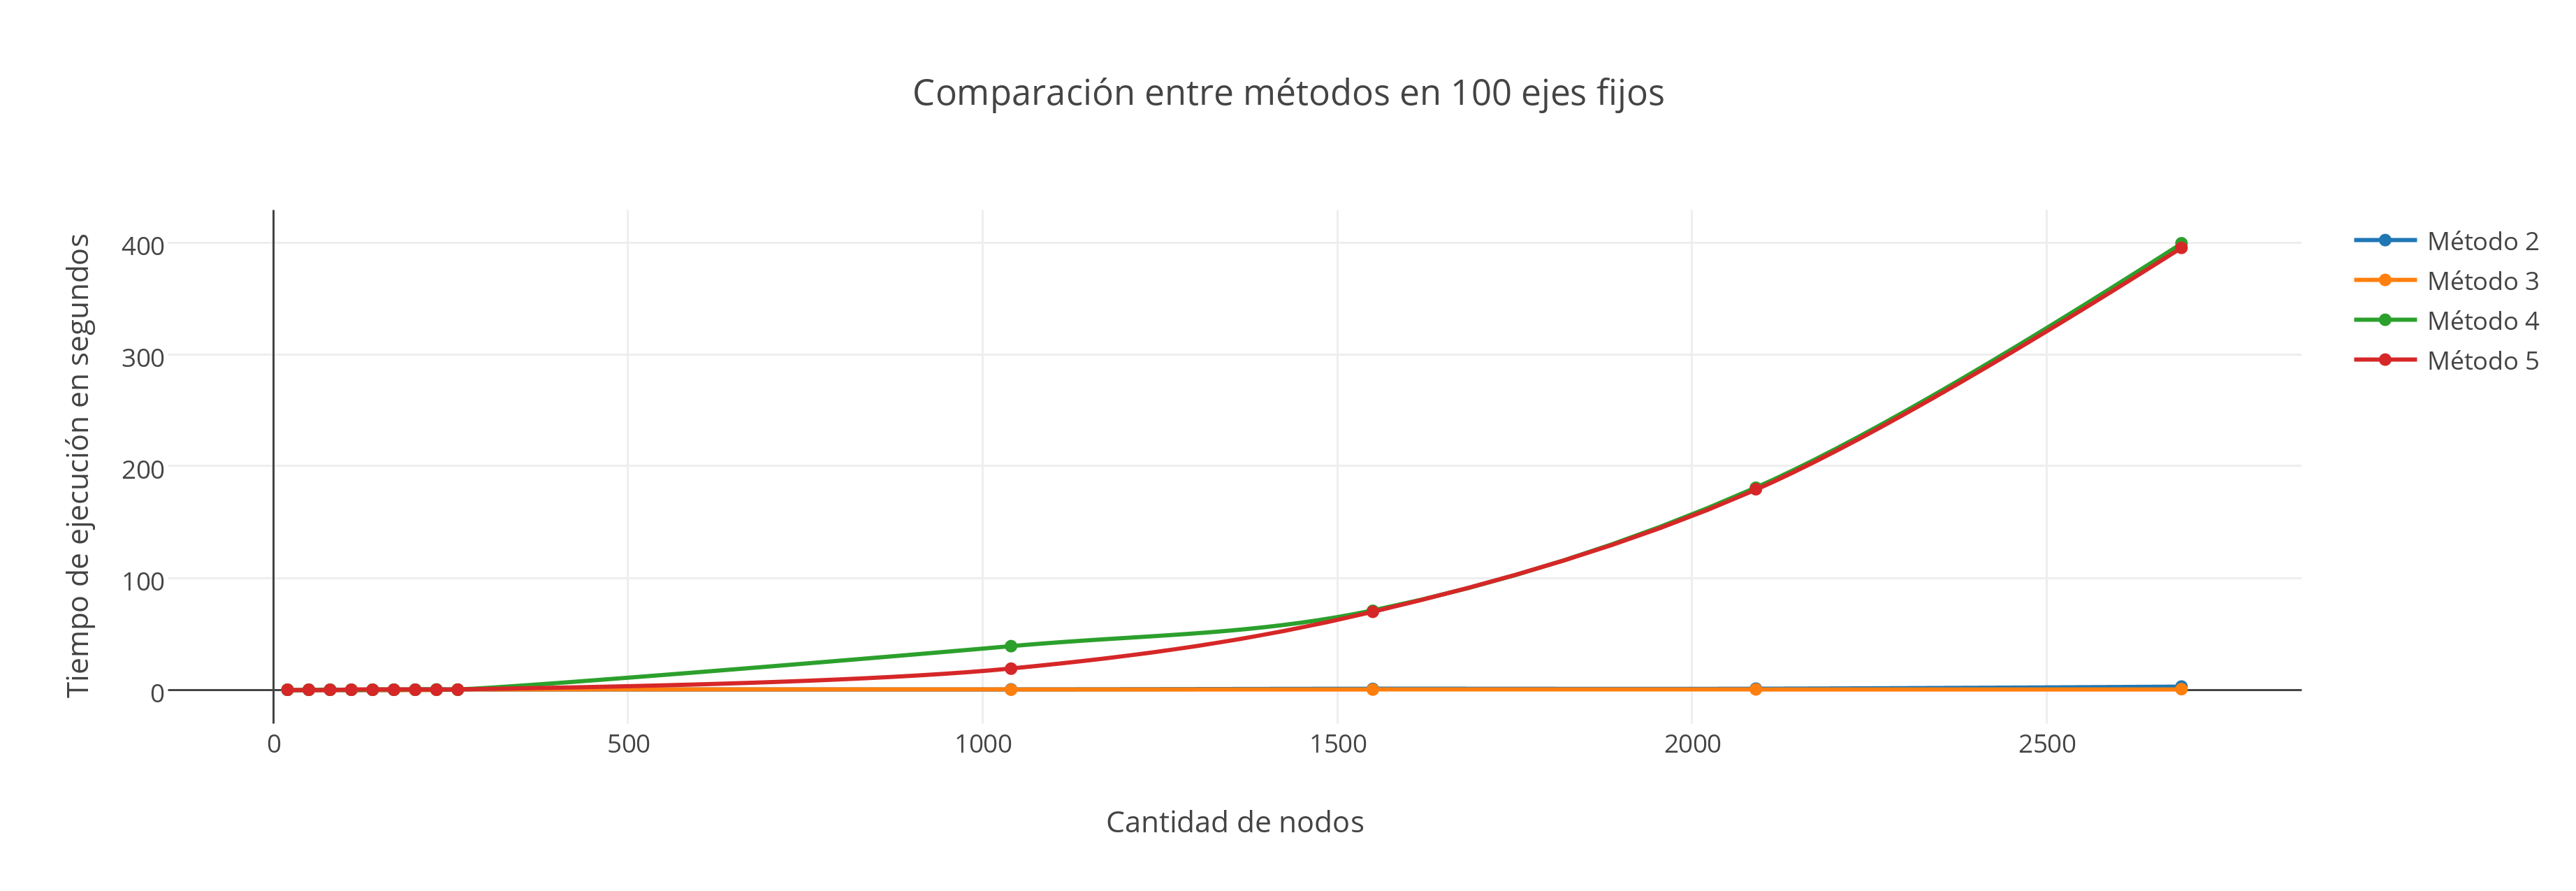
\includegraphics[scale=0.55]{imagenes/local/tiempos/100ejes.png}
% 	\caption{}
%	\label{10Nodos}
   \end{center}
 \end{figure}
 
  \begin{figure}[h!]
   \begin{center}
 	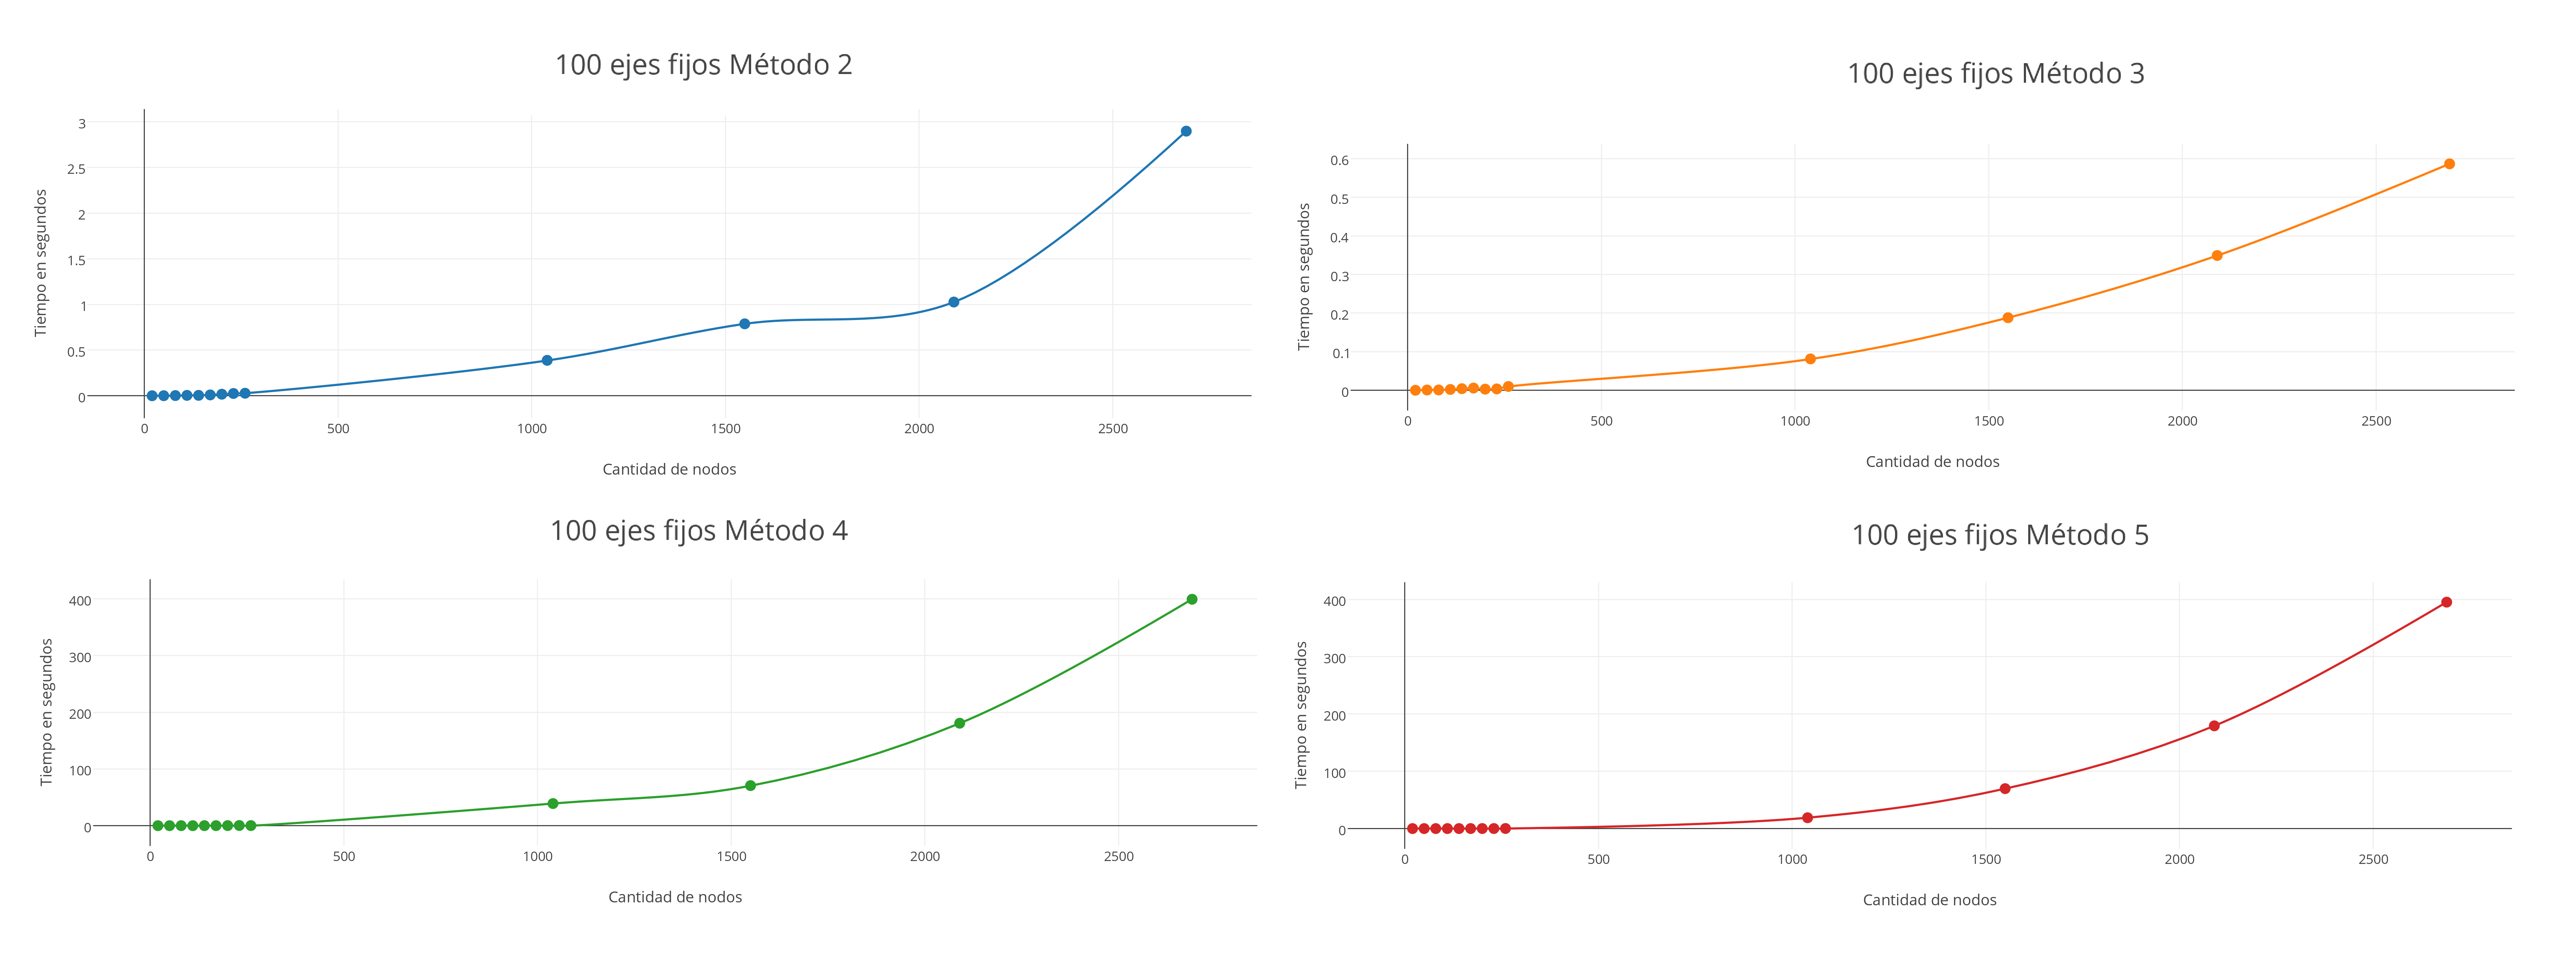
\includegraphics[scale=0.08]{imagenes/local/tiempos/100ejes2.png}
% 	\caption{}
%	\label{10Nodos}
   \end{center}
 \end{figure}

  \newpage  
 
En el primer gr\'afico se puede apreciar que cuando la cantidad de nodos comienza a ser mayor, los m\'etodos con la segunda vecindad (\textbf{4} y \textbf{5}) presentan una curva que posee un crecimiento mayor que las otras dos. Este comportamiento se condice con la complejidad te\'orica calculada ya que los m\'etodos 3 y 4 tienen una complejidad de \textcolor{red}{$O(n^6)$ (?} mientras que los primeros dos tienen \textcolor{red}{$O(n^5)$ (?}.\\

En el segundo gr\'afico lo que se quiso hacer es mostrar con detalle cada m\'etodo ya que en el primero, al tener cantidades de tiempo variadas, no se puede apreciar con detalle el comportamiento de todas las curvas por s\'i solas.

De este modo, se puede apreciar que los cuatro m\'etodos tienen un comportamiento que asemeja a una funci\'on \textcolor{red}{polinomial (? es asi?? nunca me acuerdo eso!)} aunque a simple vista no se podr\'ia acertar que sean las mismas funciones nombradas como complejidad.

\bigskip  
  
  \begin{figure}[h!]
   \begin{center}
 	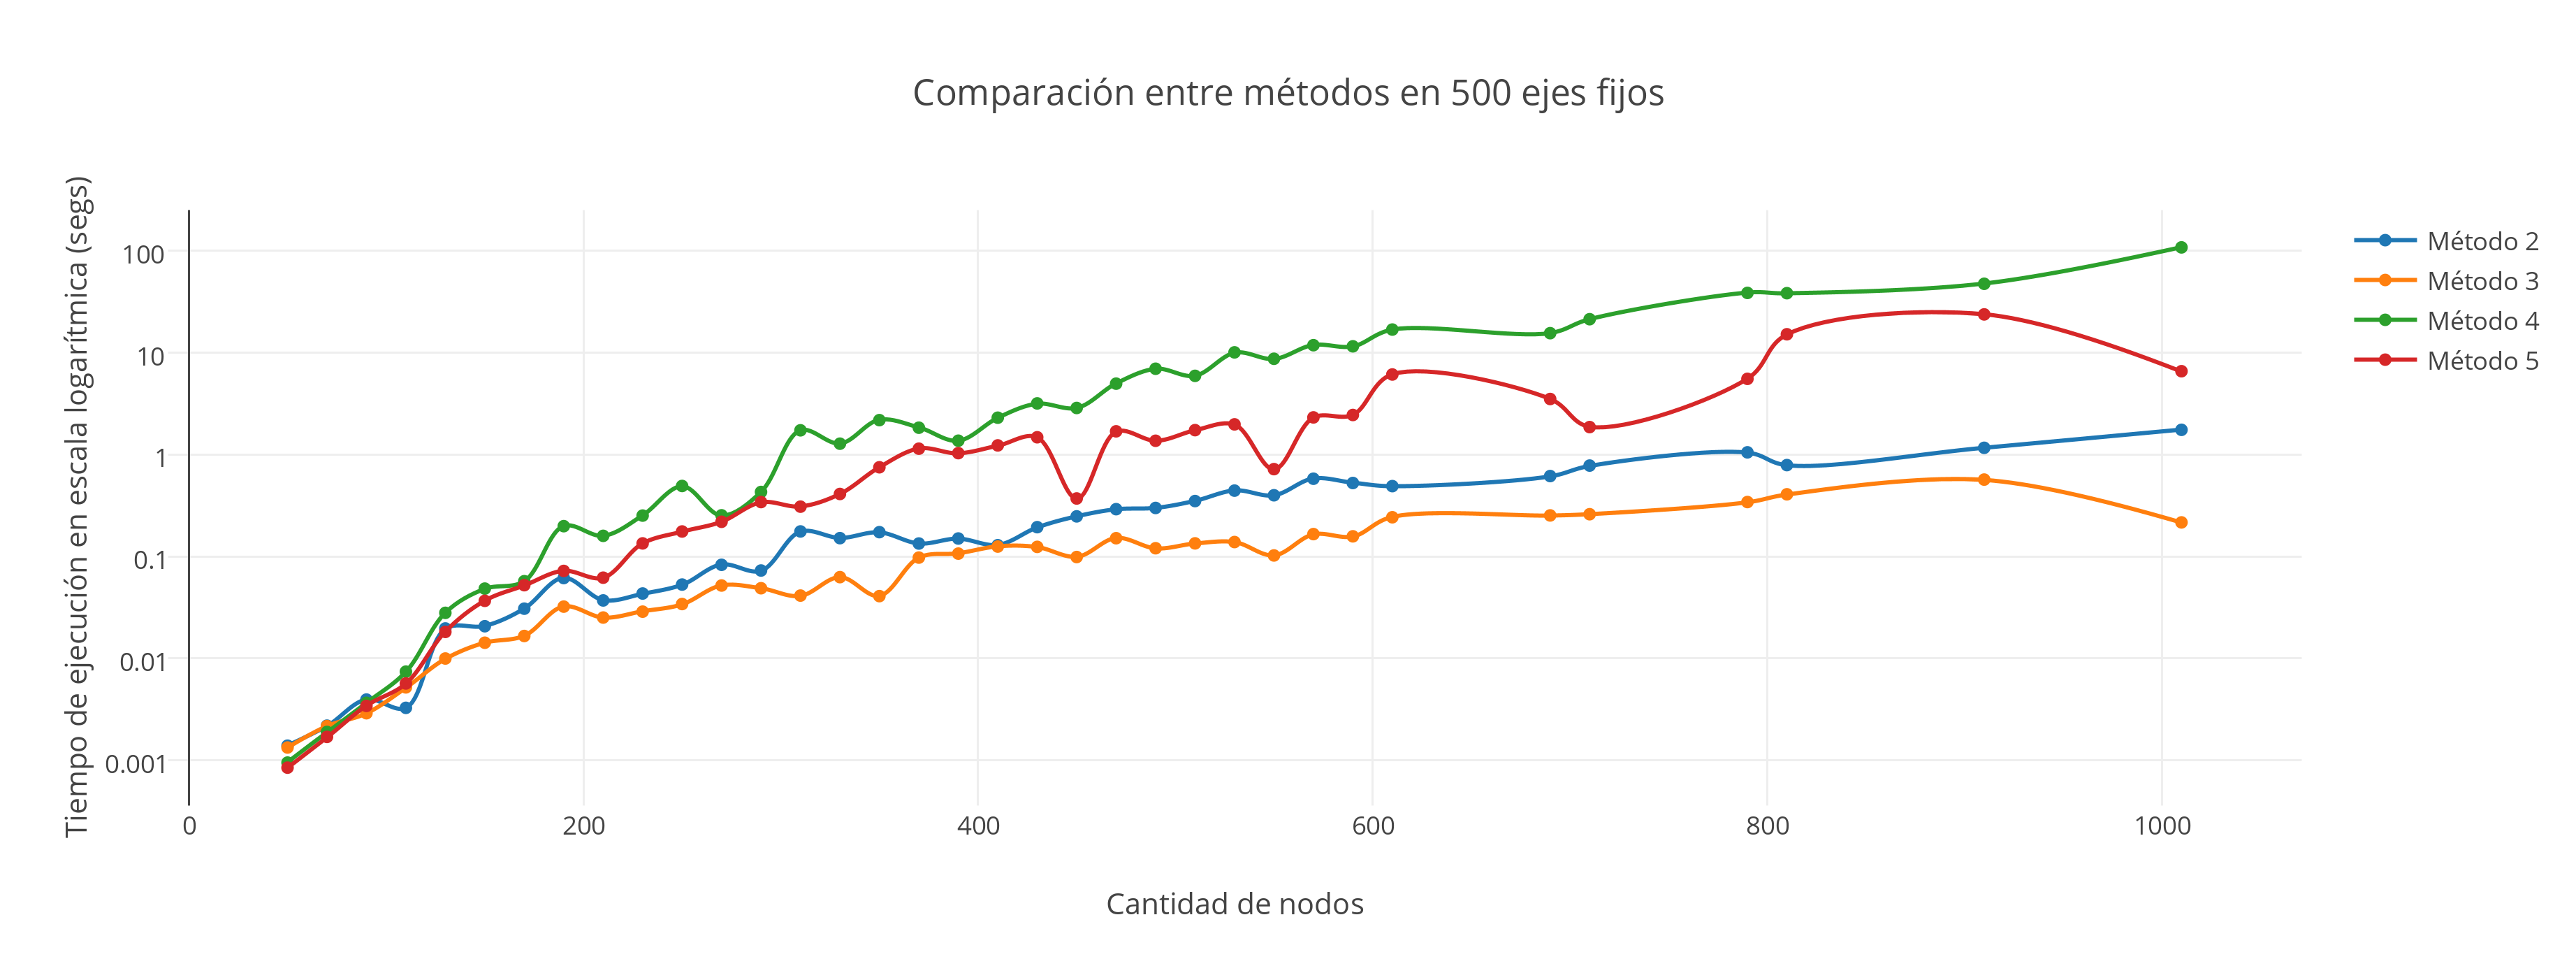
\includegraphics[scale=0.55]{imagenes/local/tiempos/500ejes.png}
% 	\caption{}
%	\label{10Nodos}
   \end{center}
 \end{figure}
 
   \begin{figure}[h!]
   \begin{center}
 	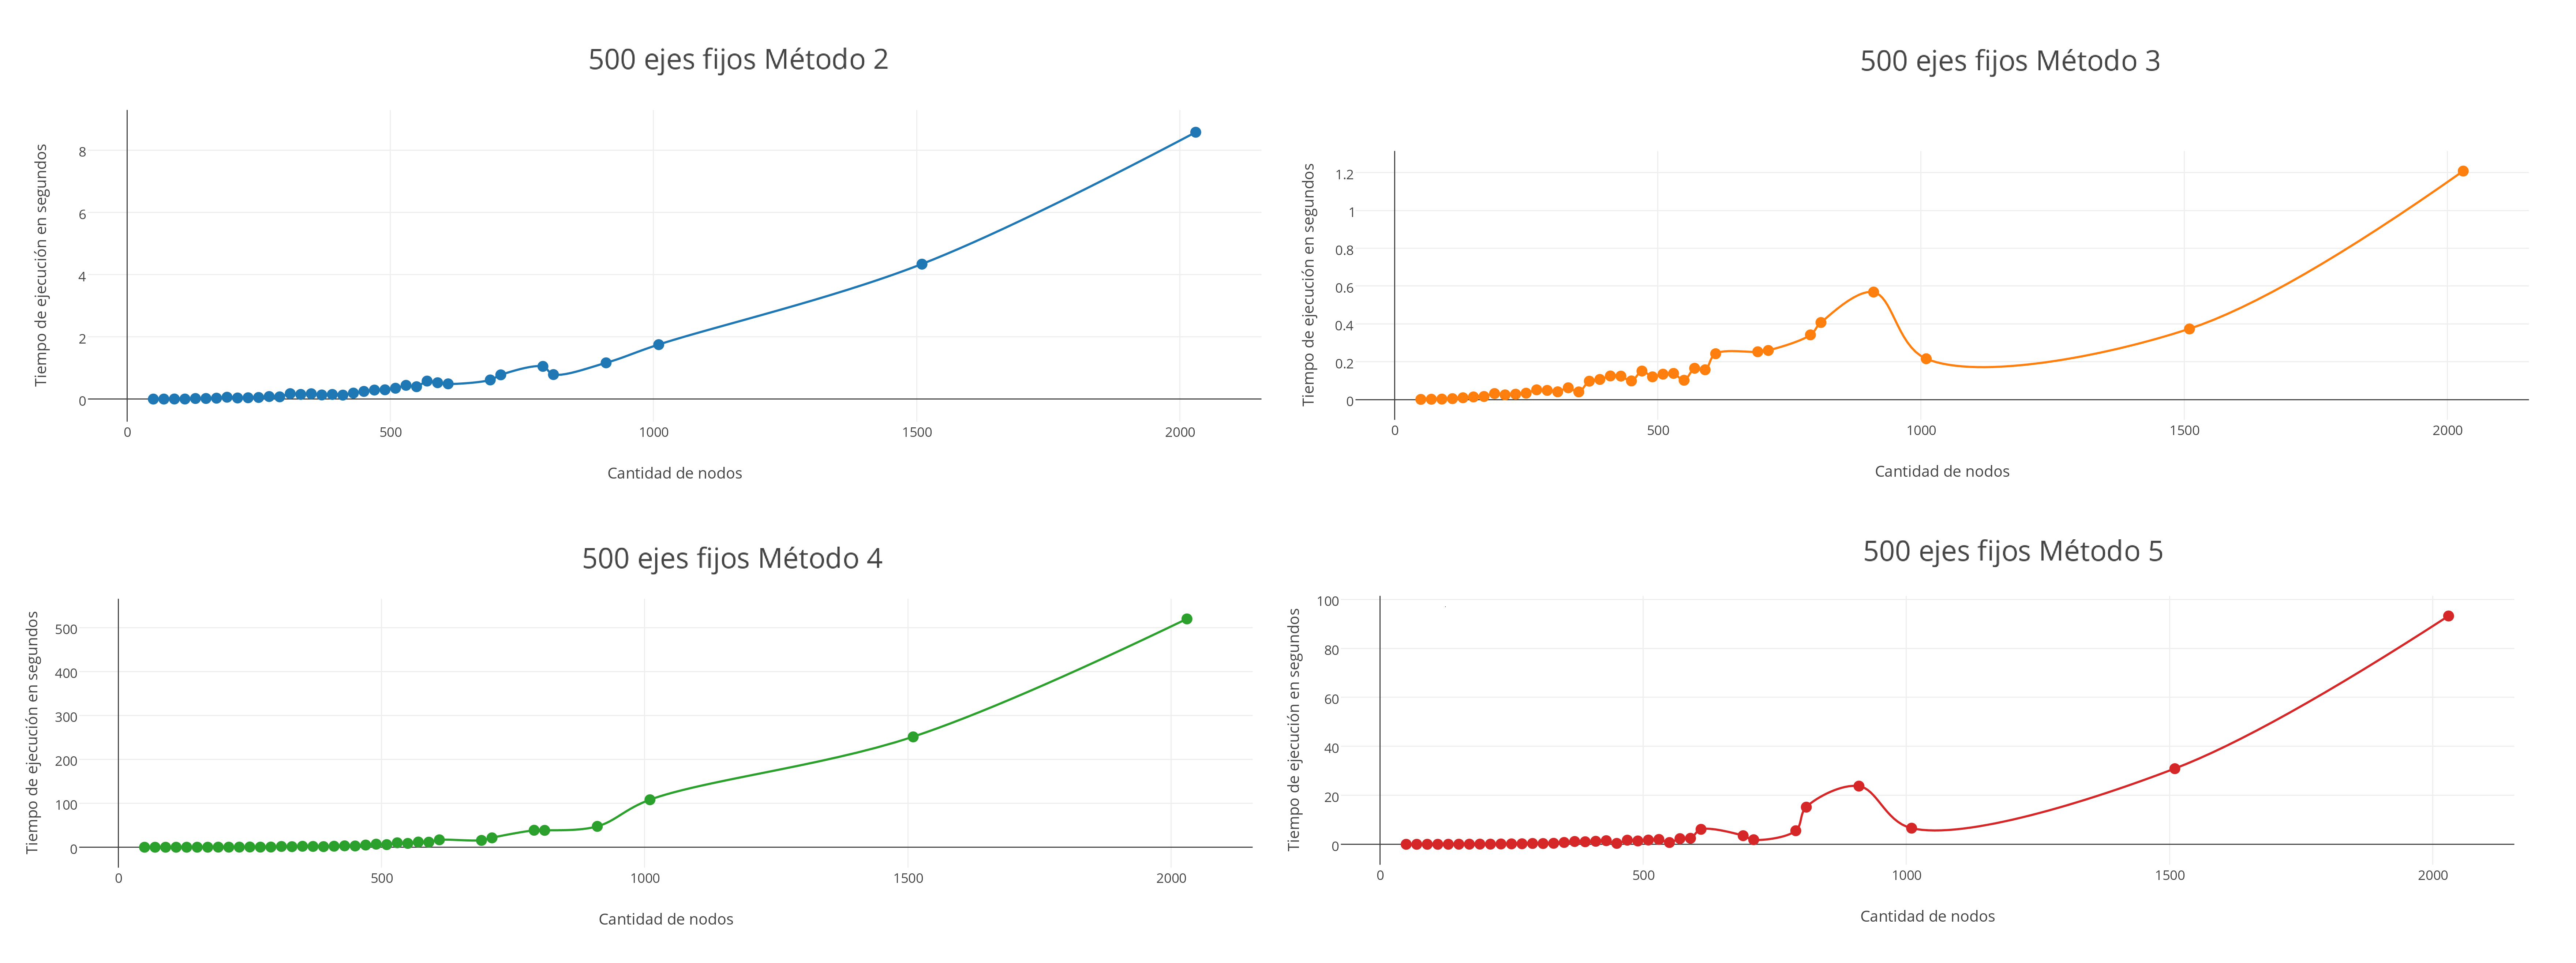
\includegraphics[scale=0.08]{imagenes/local/tiempos/500ejes2.png}
% 	\caption{}
%	\label{10Nodos}
   \end{center}
 \end{figure}

Al realizar el mismo procedimiento pero ahora con 500 ejes fijos lo que se puede apreciar es que, si bien los m\'etodos 3 y 4 se mantienen en las mediciones de tiempos mayores, la curva del \textbf{M\'etodo 4} se aleja notablemente de los dem\'as.\\

En las ampliaciones de los m\'etodos, desde una perspectiva amplia, se puede notar que poseen un comportamiento que asimila \textcolor{red}{polinomial} al igual que en el caso anterior. Se podr\'ia decir que la causa de que las gr\'aficas no sean estr\'ictamente creciente se debe a la complejidad $O(n^5)$ y $O(n^6)$.

\newpage

   \begin{figure}[h!]
   \begin{center}
 	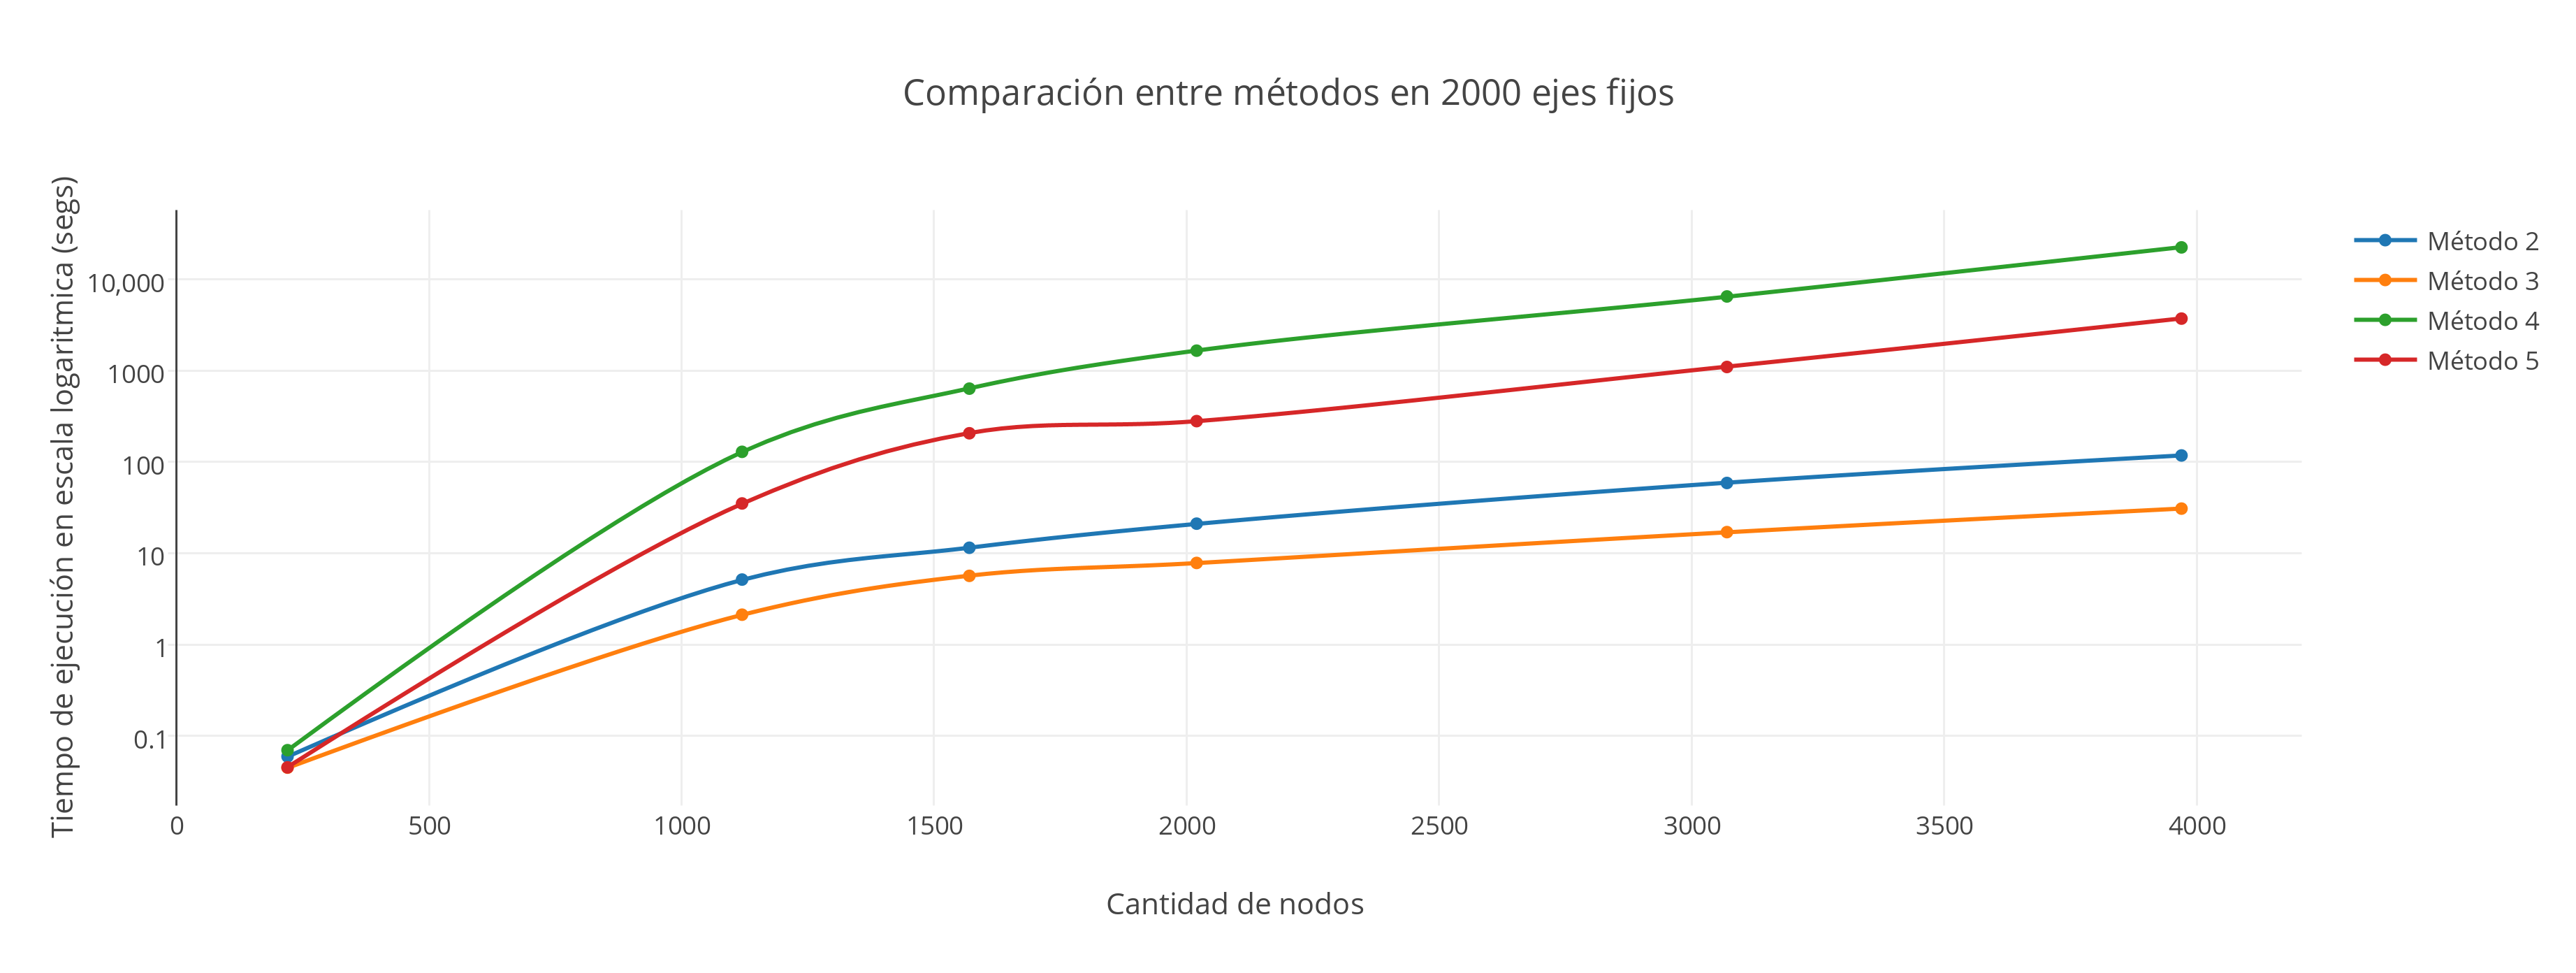
\includegraphics[scale=0.55]{imagenes/local/tiempos/2000ejes.png}
% 	\caption{}
%	\label{10Nodos}
   \end{center}
 \end{figure}
 
  \begin{figure}[h!]
   \begin{center}
 	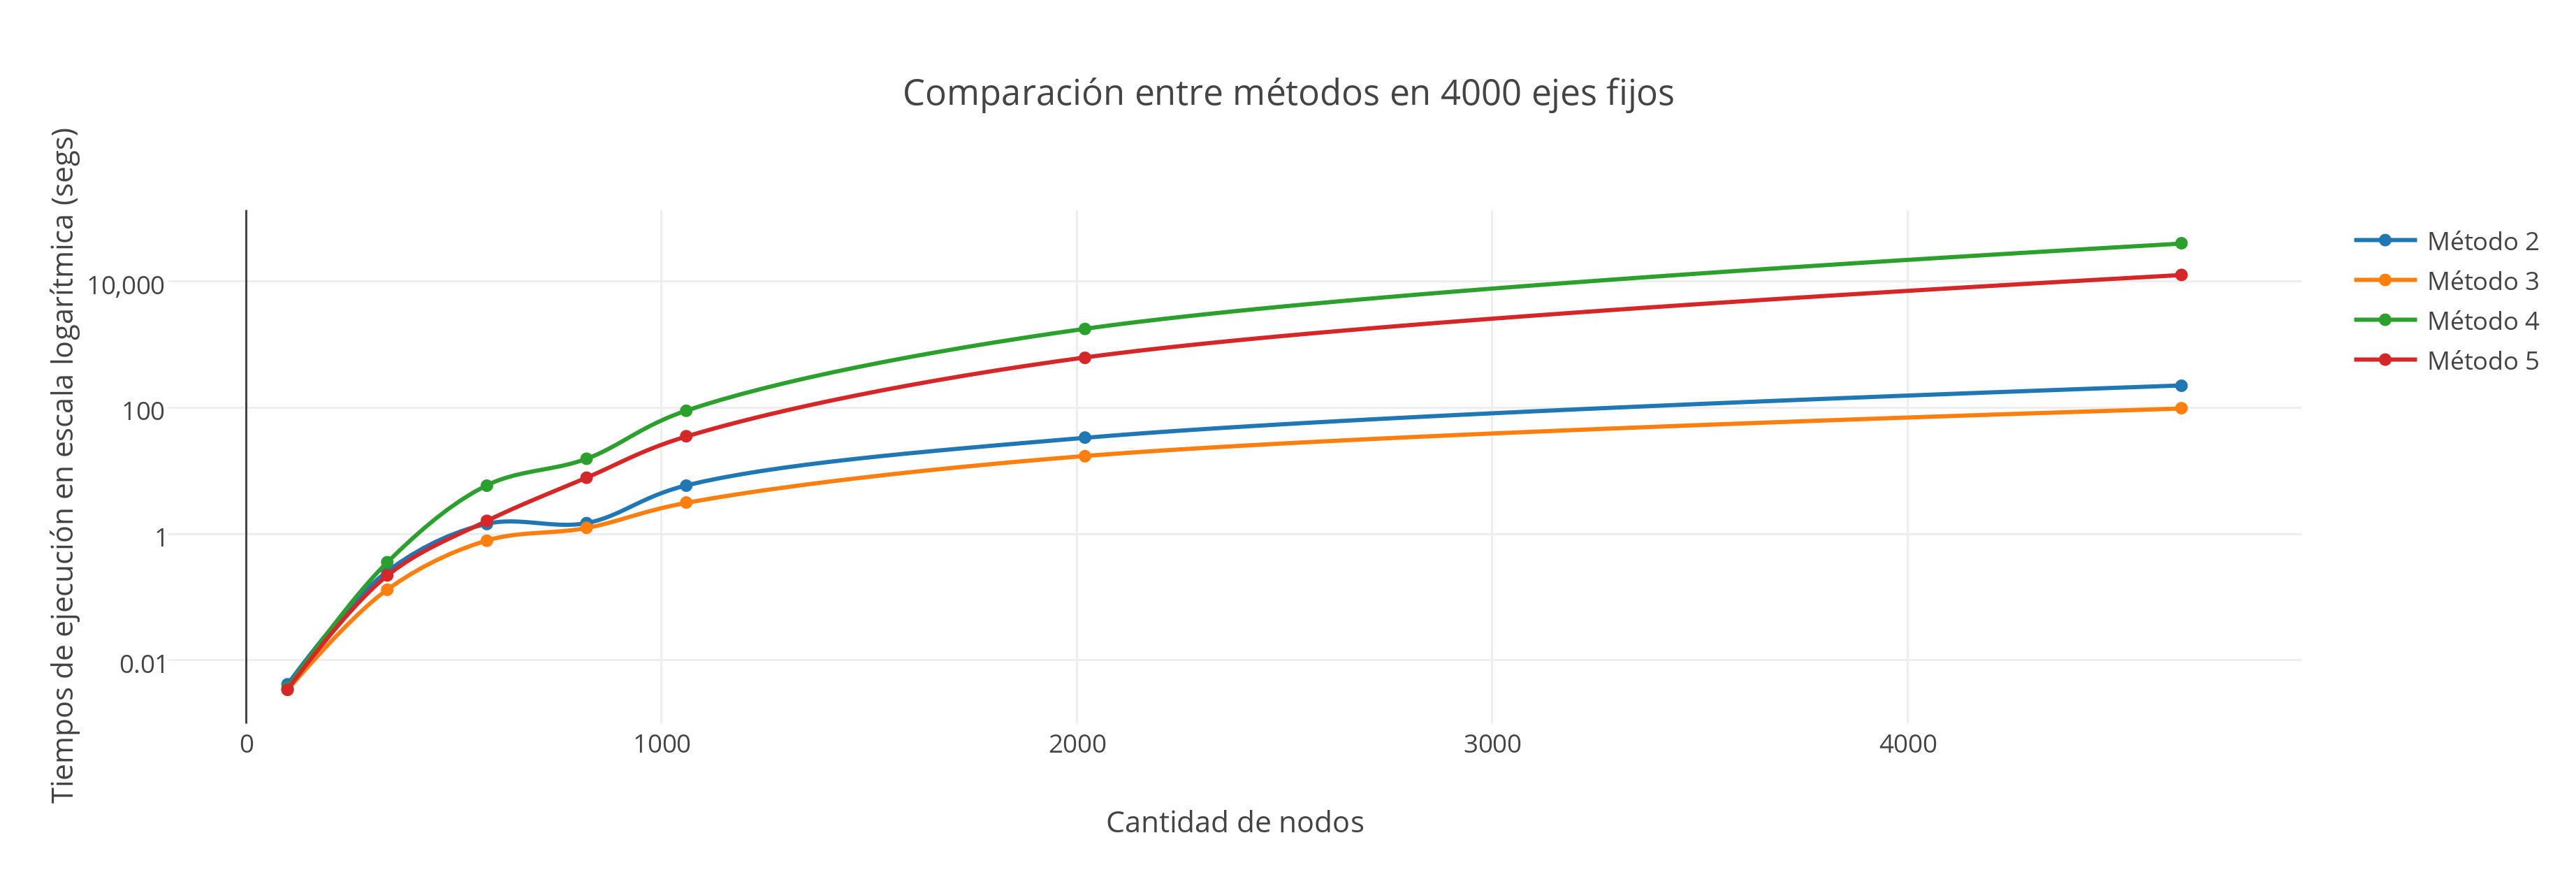
\includegraphics[scale=0.55]{imagenes/local/tiempos/4000ejes.png}
% 	\caption{}
%	\label{10Nodos}
   \end{center}
 \end{figure}
  
Al plantear la misma experimentaci\'on con cantidad de ejes mayor, se puede apreciar un comportamiento an\'alogo donde el \textbf{m\'etodo 4} posee un tiempo de ejecuci\'on notablemente mayor al resto y el \textbf{m\'etodo 3} permanece siendo el de menor tiempo de ejecuci\'on.  
  
 \newpage  
  
\subsubsection*{Nodos Fijos}

En esta instancia, se contrastar\'an grupos de grafos que posean cantidad de nodos fijos: 200, 300, 500, 600 y 700 variando en cada caso la cantidad de ejes. Se comparan los tiempos de ejecuci\'on entre los cuatro m\'etodos planteados en los casos generados. 

  \begin{figure}[h!]
   \begin{center}
 	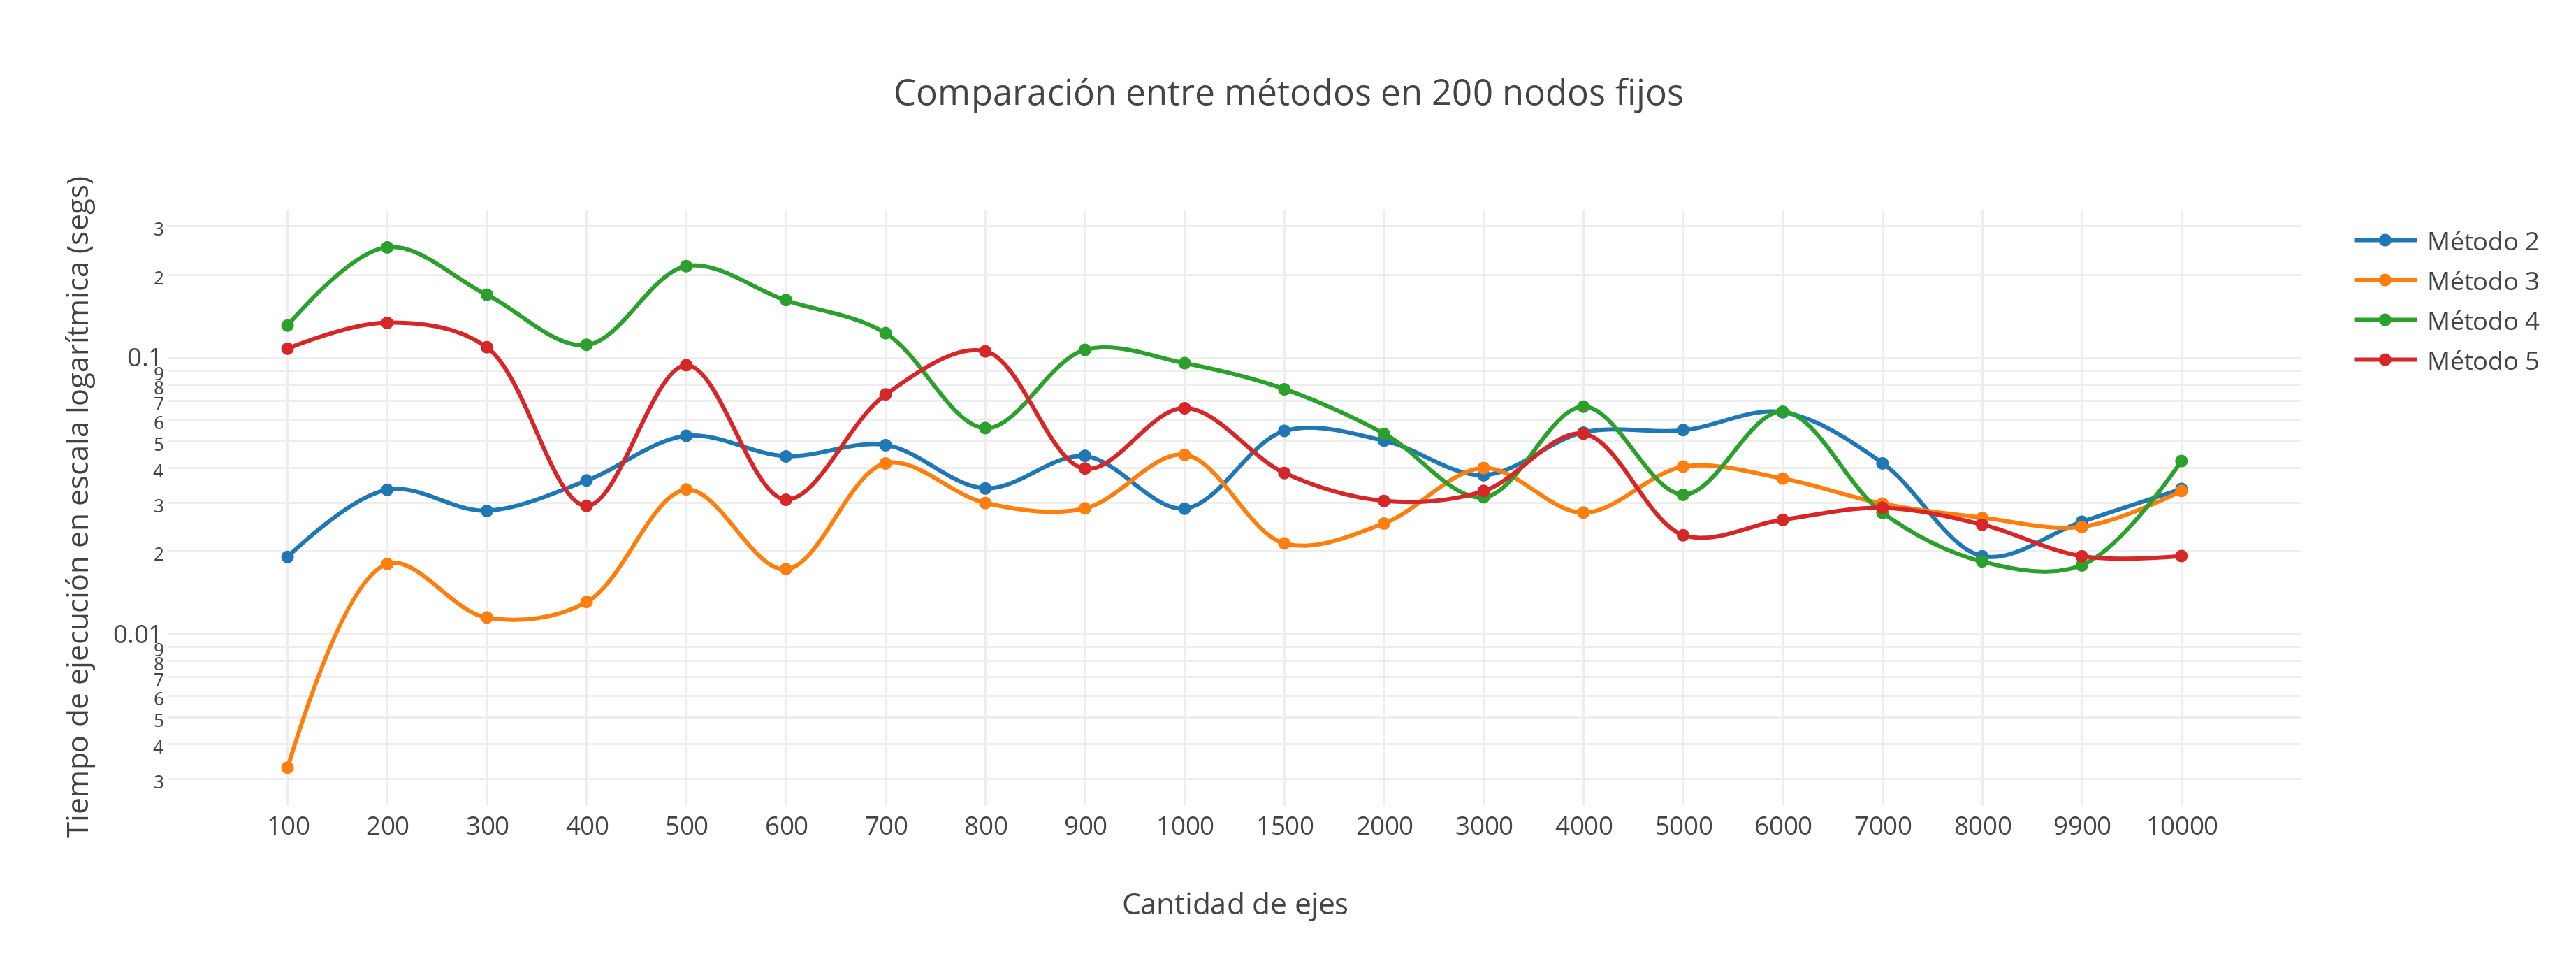
\includegraphics[scale=0.55]{imagenes/local/tiempos/200nodos.png}
% 	\caption{}
%	\label{10Nodos}
   \end{center}
 \end{figure}
 
Dando una observaci\'on general sobre este gr\'afico, se puede apreciar que para todos los m\'etodos el tiempo de ejecuci\'on disminuye al aumentar la cantidad de ejes. \\

A simple vista podr\'ia sonar un poco absurdo, sin embargo la causa de este comportamiento  est\'a ligada a que al existir mayor cantidad de ejes (manteniendo la cantidad de nodos) aumenta el grado de los nodos. Por lo tanto\textcolor{red}{, al igual que el algoritmo Goloso(?), } cuando se arma una soluci\'on inicial se inserta el nodo de mayor grado. Luego, se descartan todos los nodos vecinos ya que no ser\'an candidatos al conjunto soluci\'on.

Si bien, para descartar nodos vecinos, se debe recorrer la lista de adyacencia completa; ese tiempo es compensado al tener menos nodos en la siguiente iteraci\'on para recorrer.\\

En cuanto a la parte del algoritmo que consiste en la b\'usqueda local, \textcolor{red}{Completar algo aca...}

   \begin{figure}[h!]
   \begin{center}
 	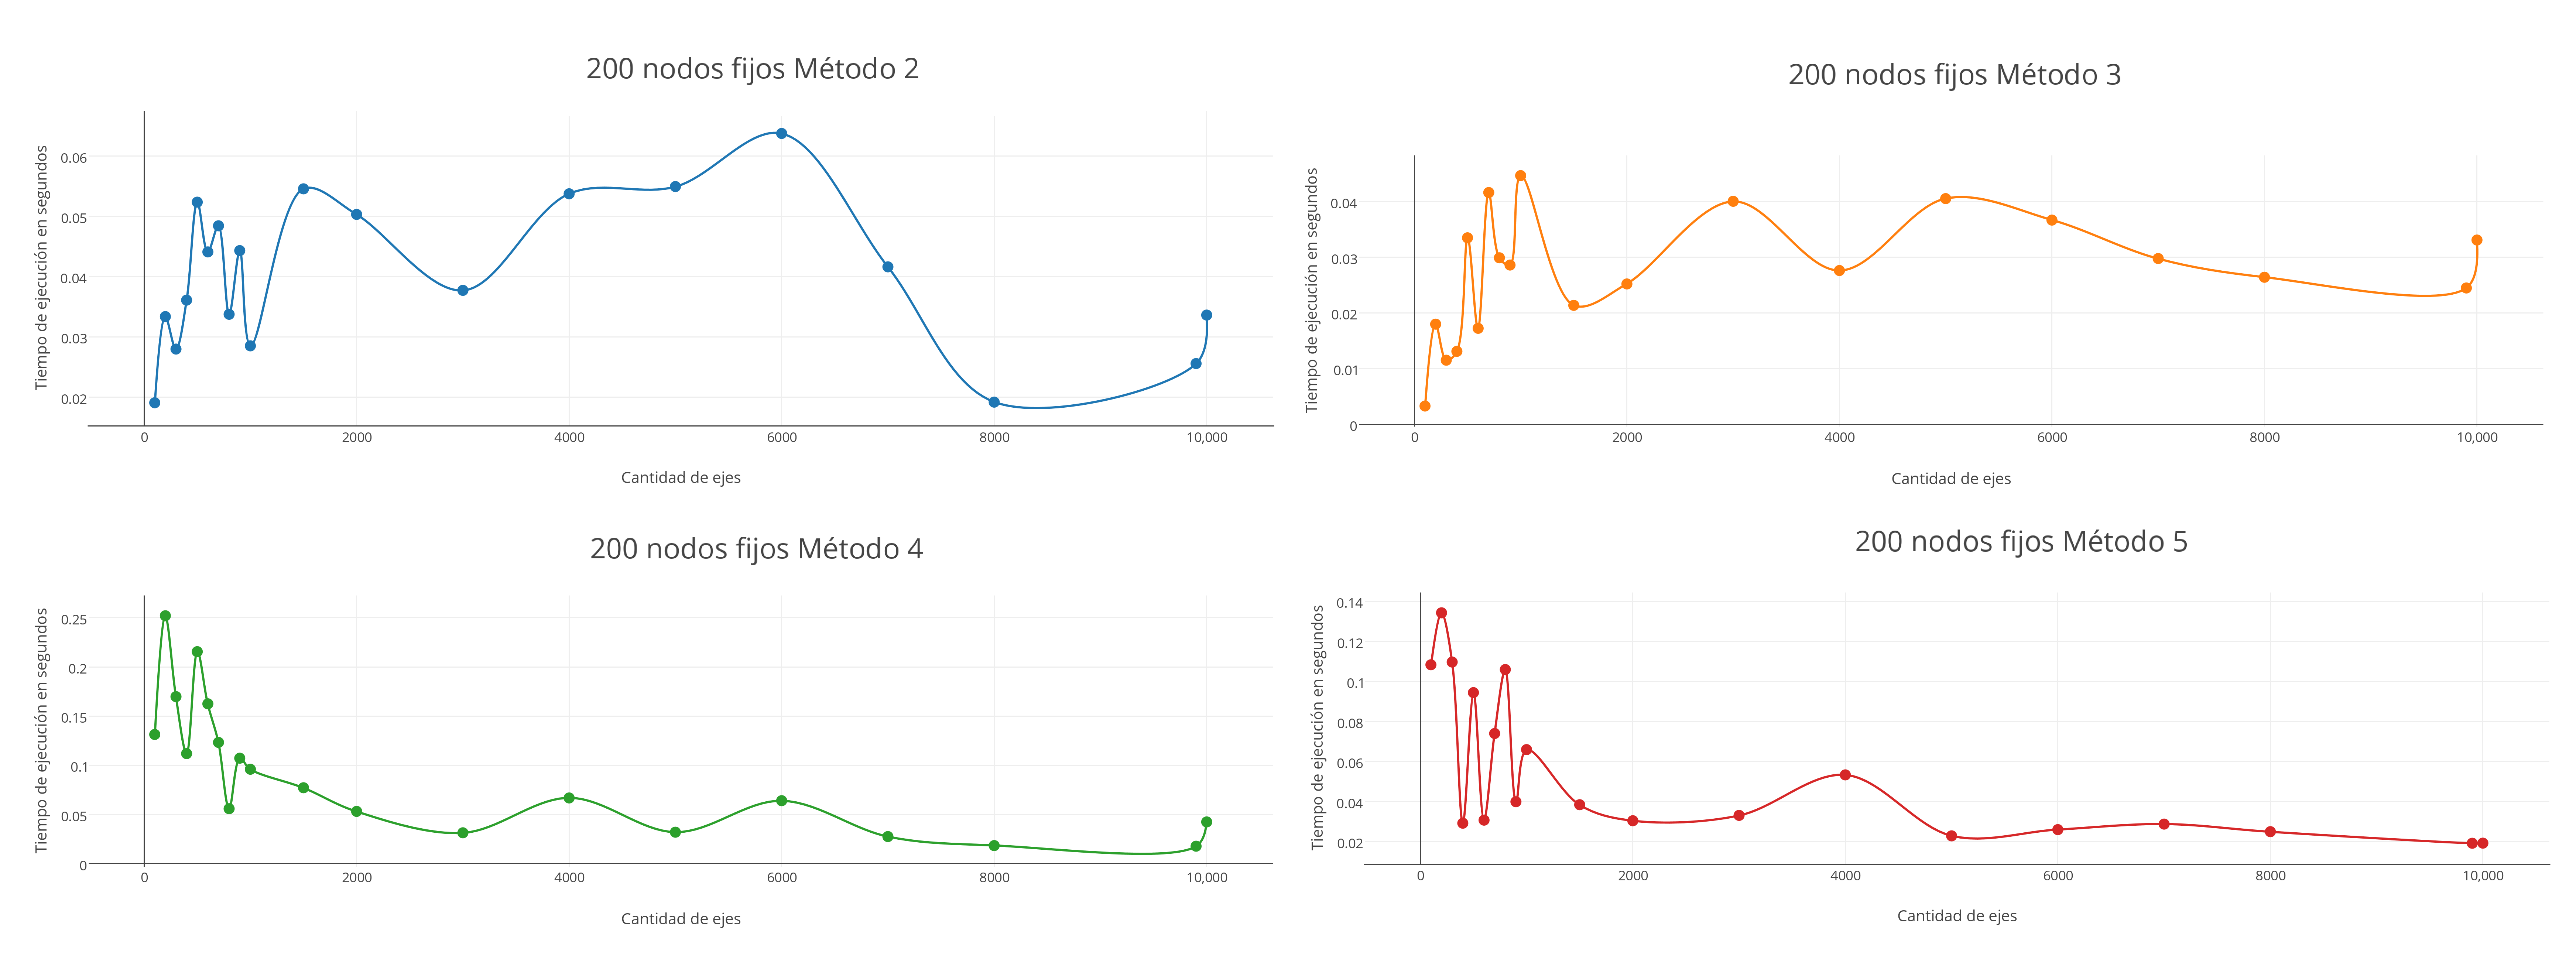
\includegraphics[scale=0.08]{imagenes/local/tiempos/200nodos2.png}
% 	\caption{}
%	\label{10Nodos}
   \end{center}
 \end{figure}
 
 Haciendo hincapie en cada m\'etodo por separado, se observa un comportamiento distinguible.\\
 
 Si bien las curvas de los cuatro m\'etodos oscilan notablemente, si uno observa bajo un punto de vista general se puede apreciar que los m\'etodos 4 y 5 tienen un comportamiento notablemente decreciente similar al de una curva \textcolor{red}{polinomial (?}. Ambos m\'etodos utilizan la segunda vecindad, lo que indicar\'ia que el comportamiento es causado por \textcolor{red}{completar!!!}.\\
 
 Por otro lado, los m\'etodos 3 y 4 poseen un crecimiento abrupto con una cantidad de ejes menor y despu\'es sus curvas oscilan de manera, se podr\'ia decir que, constante. Como ambas manejan la misma vecindad, un potencial causante de dicho comportamiento corresponde a ... \textcolor{red}{COMPLETAR}\\

\bigskip

Ejecutamos la misma experimentaci\'on, pero en esta ocasi\'on fijando la cantidad de nodos en 300, 500 y 600. 
 
  \begin{figure}[h!]
   \begin{center}
 	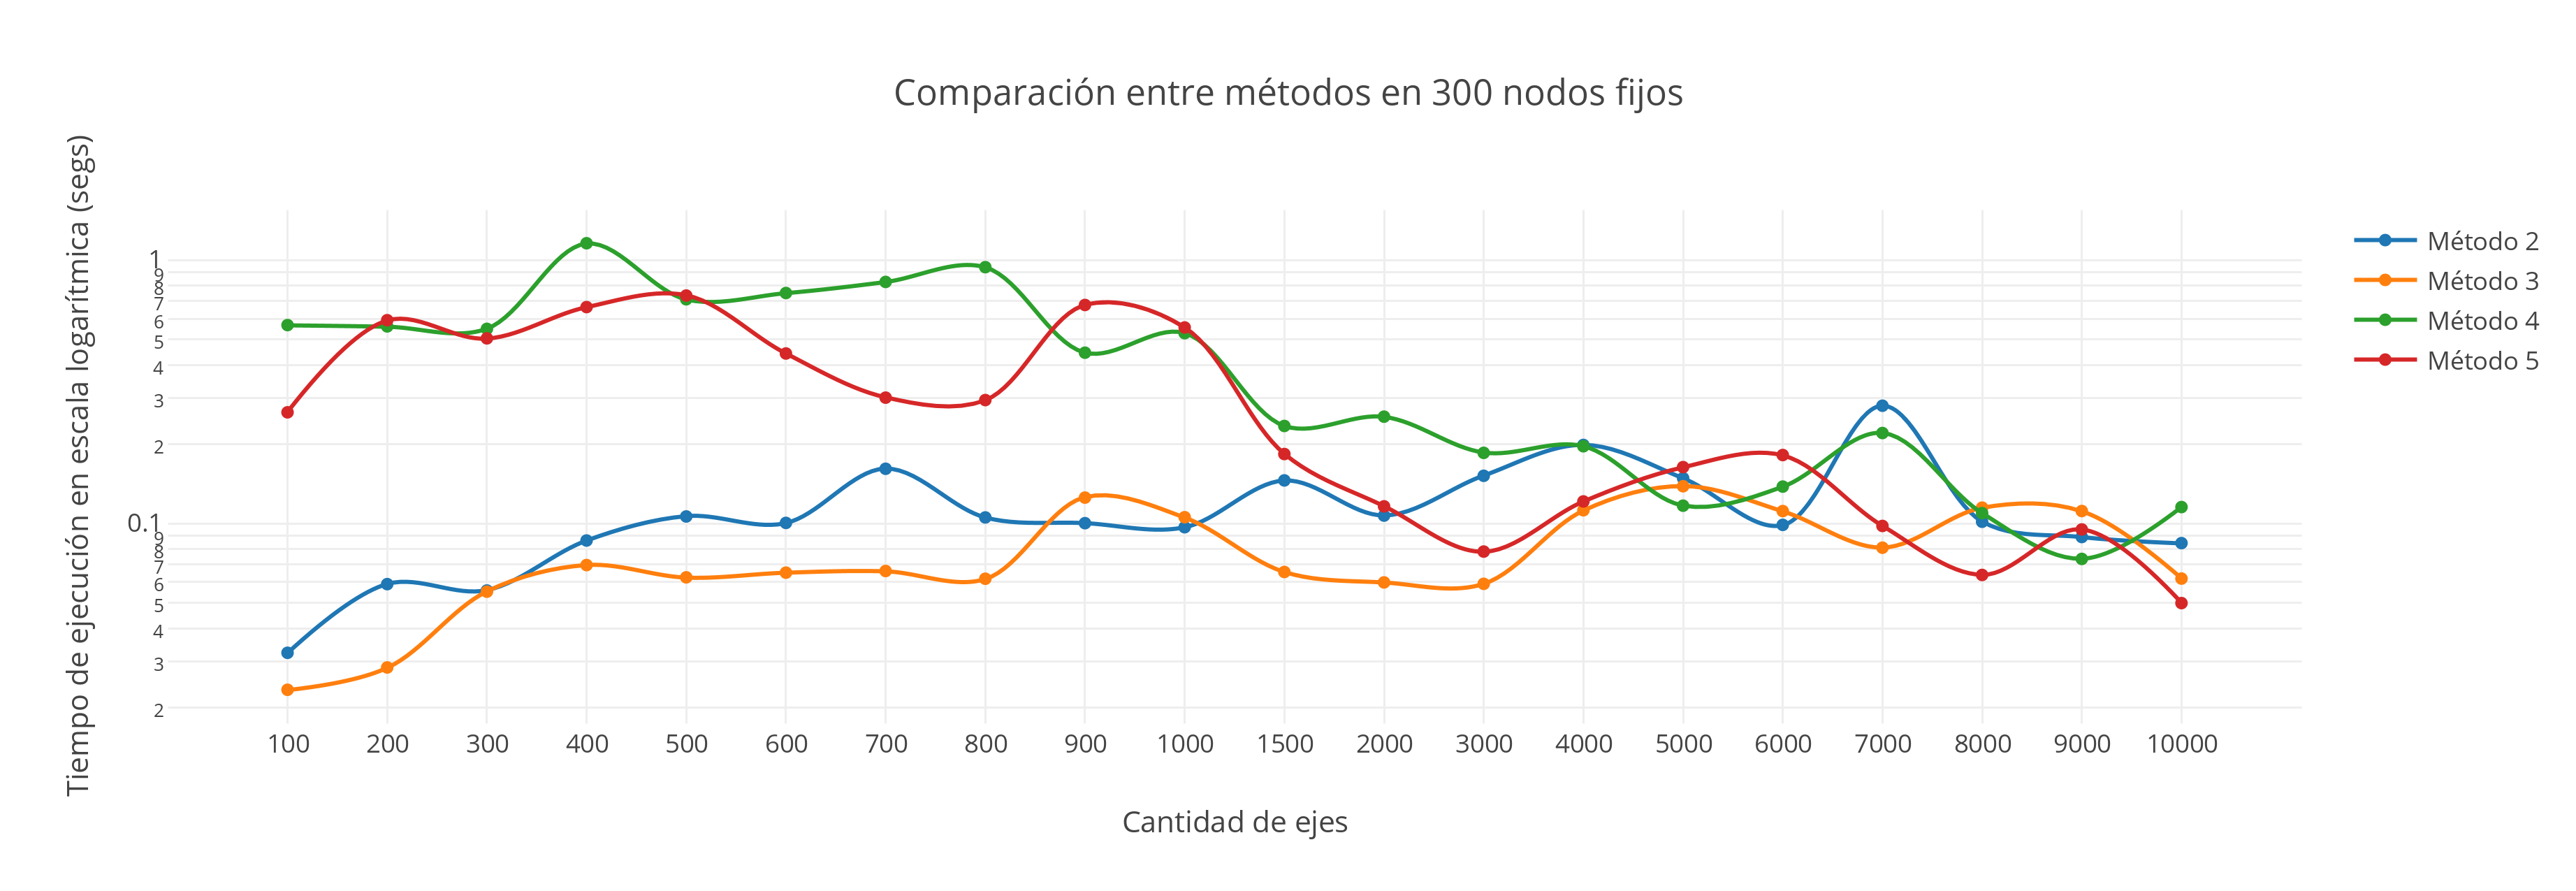
\includegraphics[scale=0.55]{imagenes/local/tiempos/300nodos.png}
% 	\caption{}
%	\label{10Nodos}
   \end{center}
 \end{figure}
 
   \begin{figure}[h!]
   \begin{center}
 	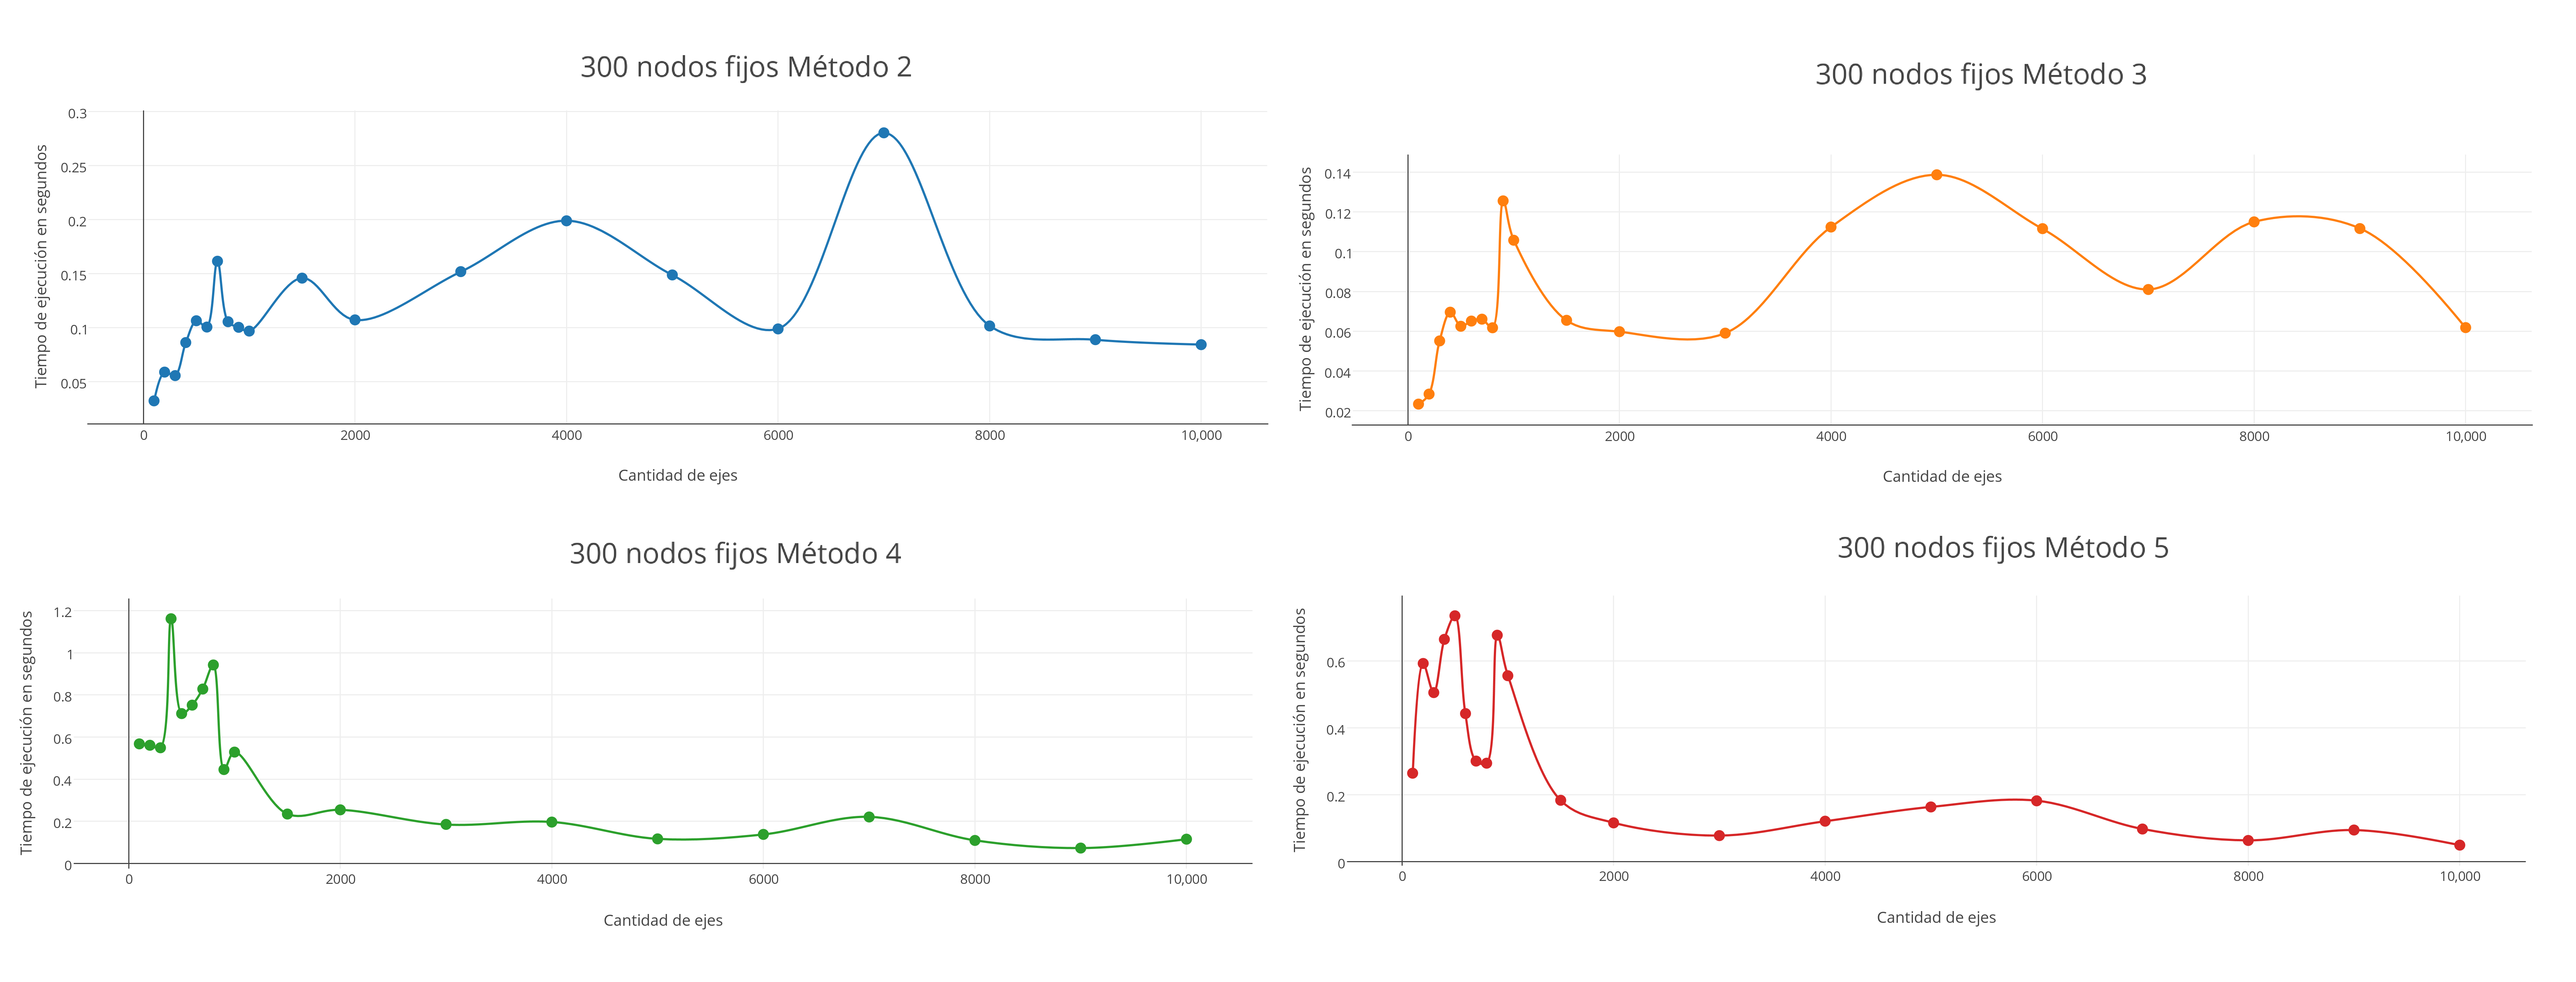
\includegraphics[scale=0.08]{imagenes/local/tiempos/300nodos2.png}
% 	\caption{}
%	\label{10Nodos}
   \end{center}
 \end{figure}



  \begin{figure}[h!]
   \begin{center}
 	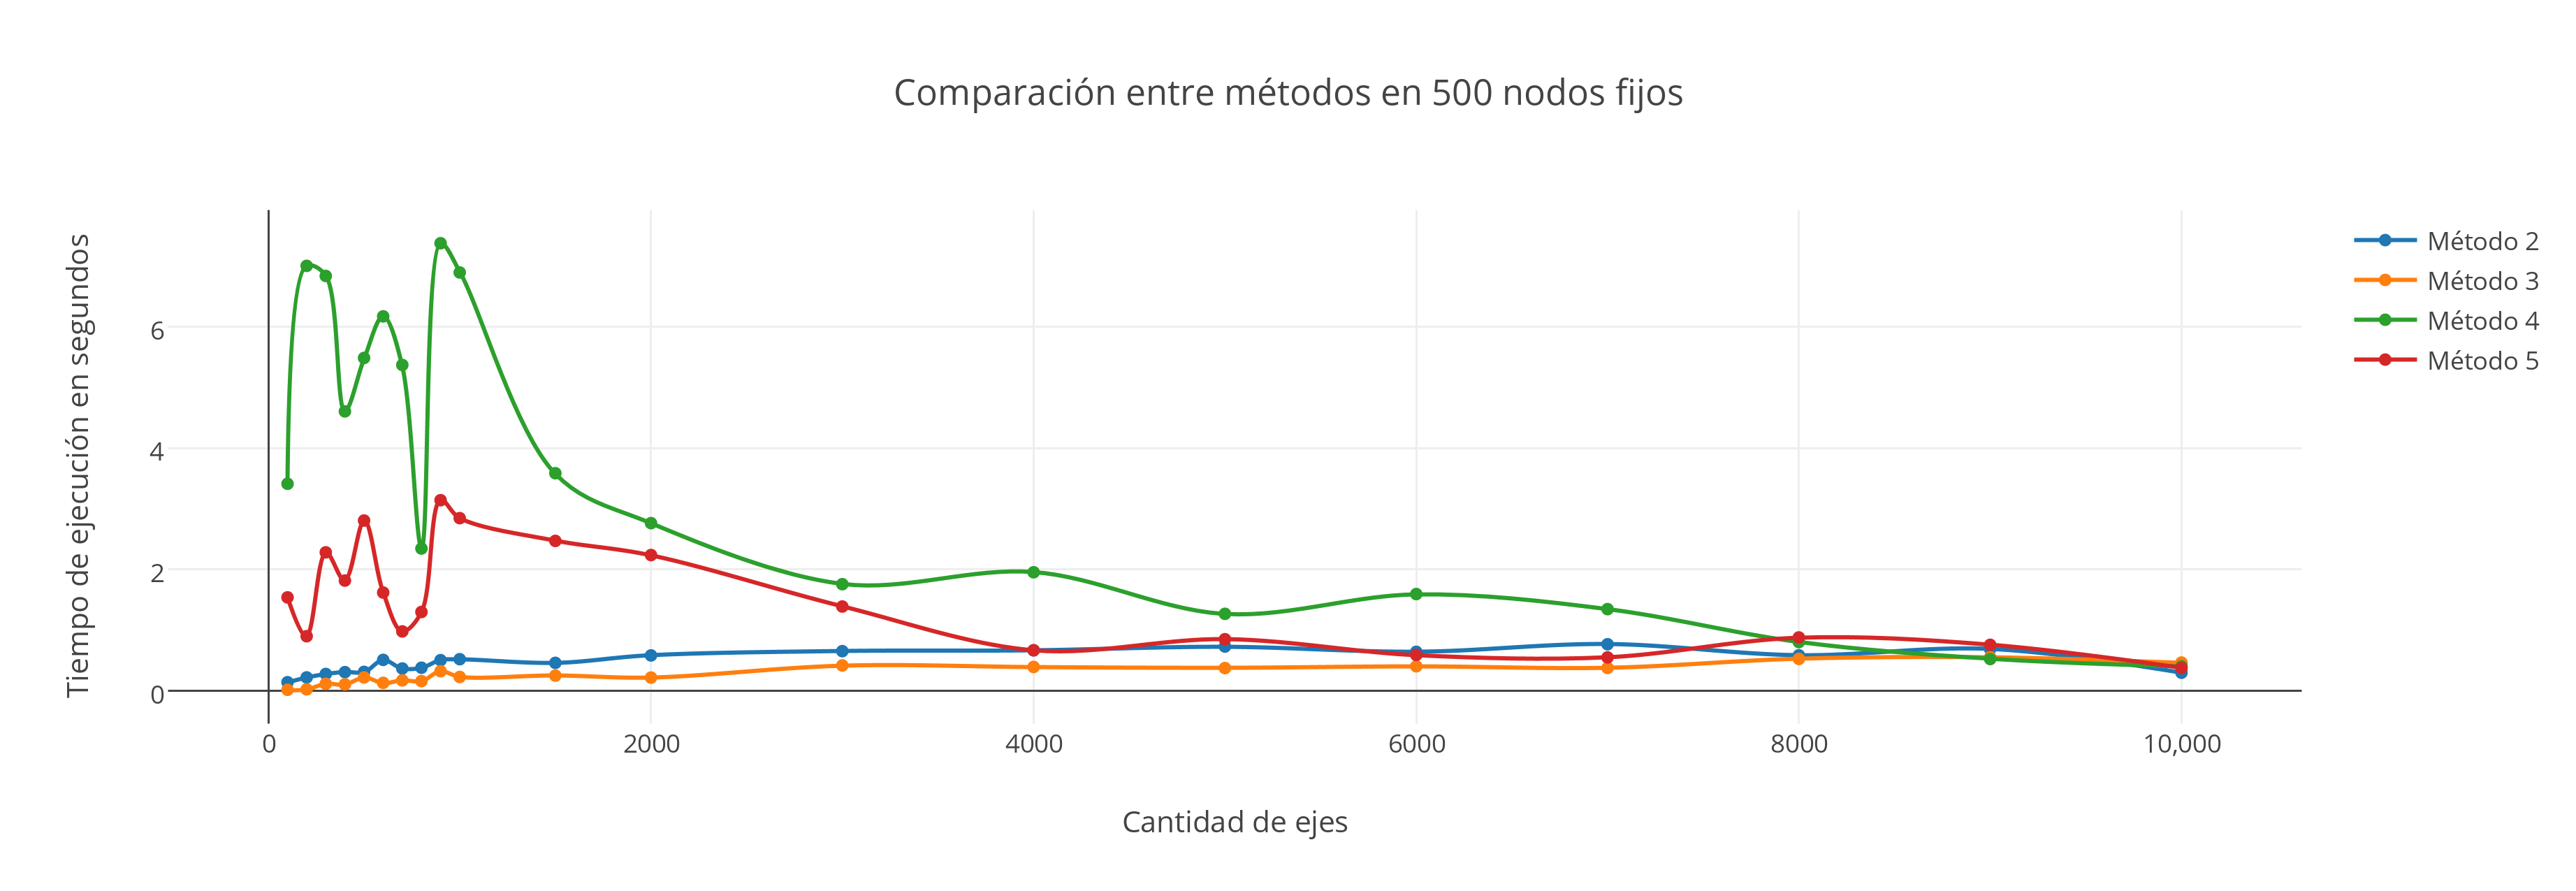
\includegraphics[scale=0.55]{imagenes/local/tiempos/500nodos.png}
% 	\caption{}
%	\label{10Nodos}
   \end{center}
 \end{figure}
 
\newpage 
 
   \begin{figure}[h!]
   \begin{center}
 	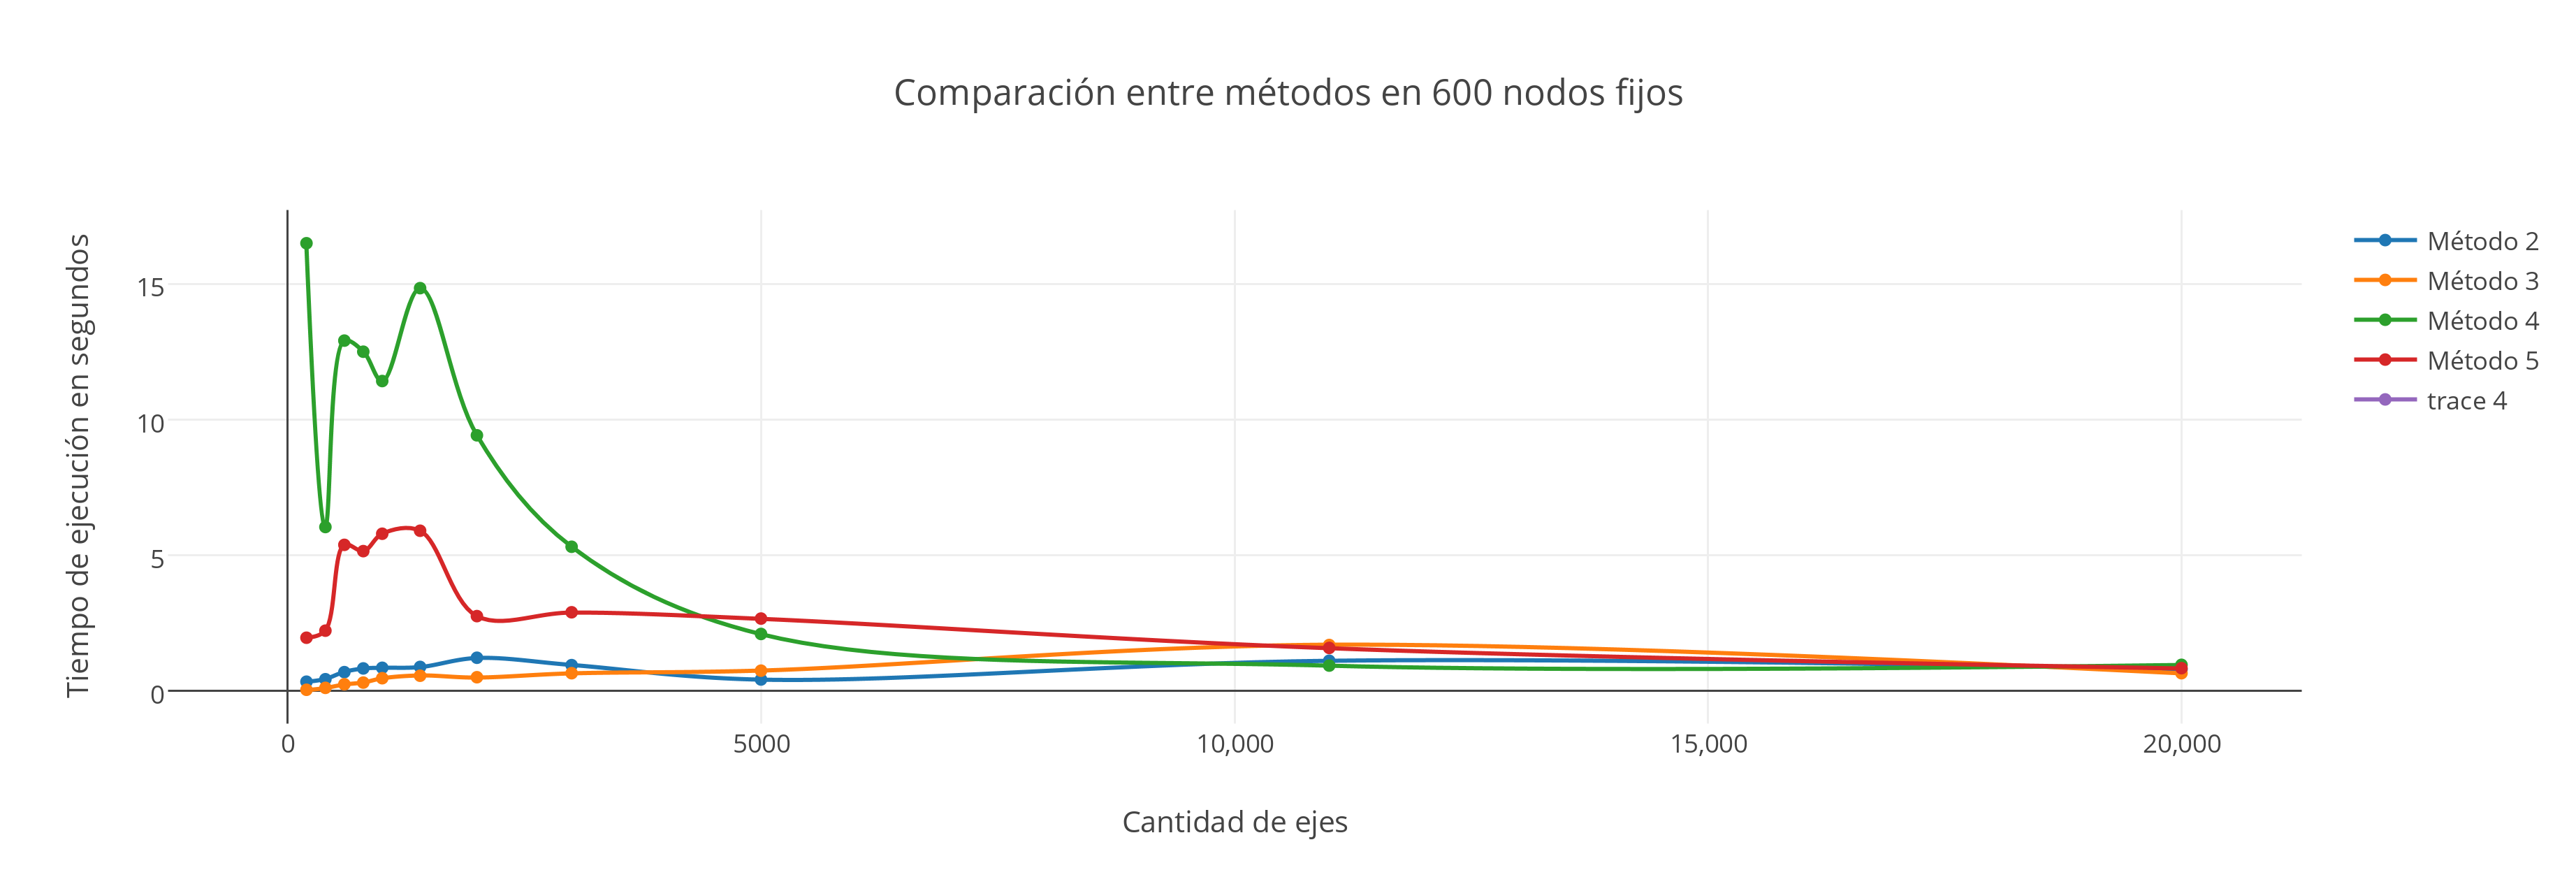
\includegraphics[scale=0.55]{imagenes/local/tiempos/600nodos.png}
% 	\caption{}
%	\label{10Nodos}
   \end{center}
 \end{figure}

La conclusi\'on que se puede sacar de este \'ultimo set de gr\'aficos es que, si se fija la cantidad de nodos, no importa en qu\'e valor, los tiempos de ejecuci\'on de los m\'etodos poseen un comportamiento similar al explicado en el inciso anterior.

Donde el \textbf{M\'etodo 4} permanece siendo quien tiene mayores tiempos de ejecuci\'on sin importar la cantidad de nodos y ejes. As\'i mismo, el \textbf{M\'etodo 3} se mantiene con los tiempos de ejecuci\'on menores.

  \begin{figure}[h!]
   \begin{center}
 	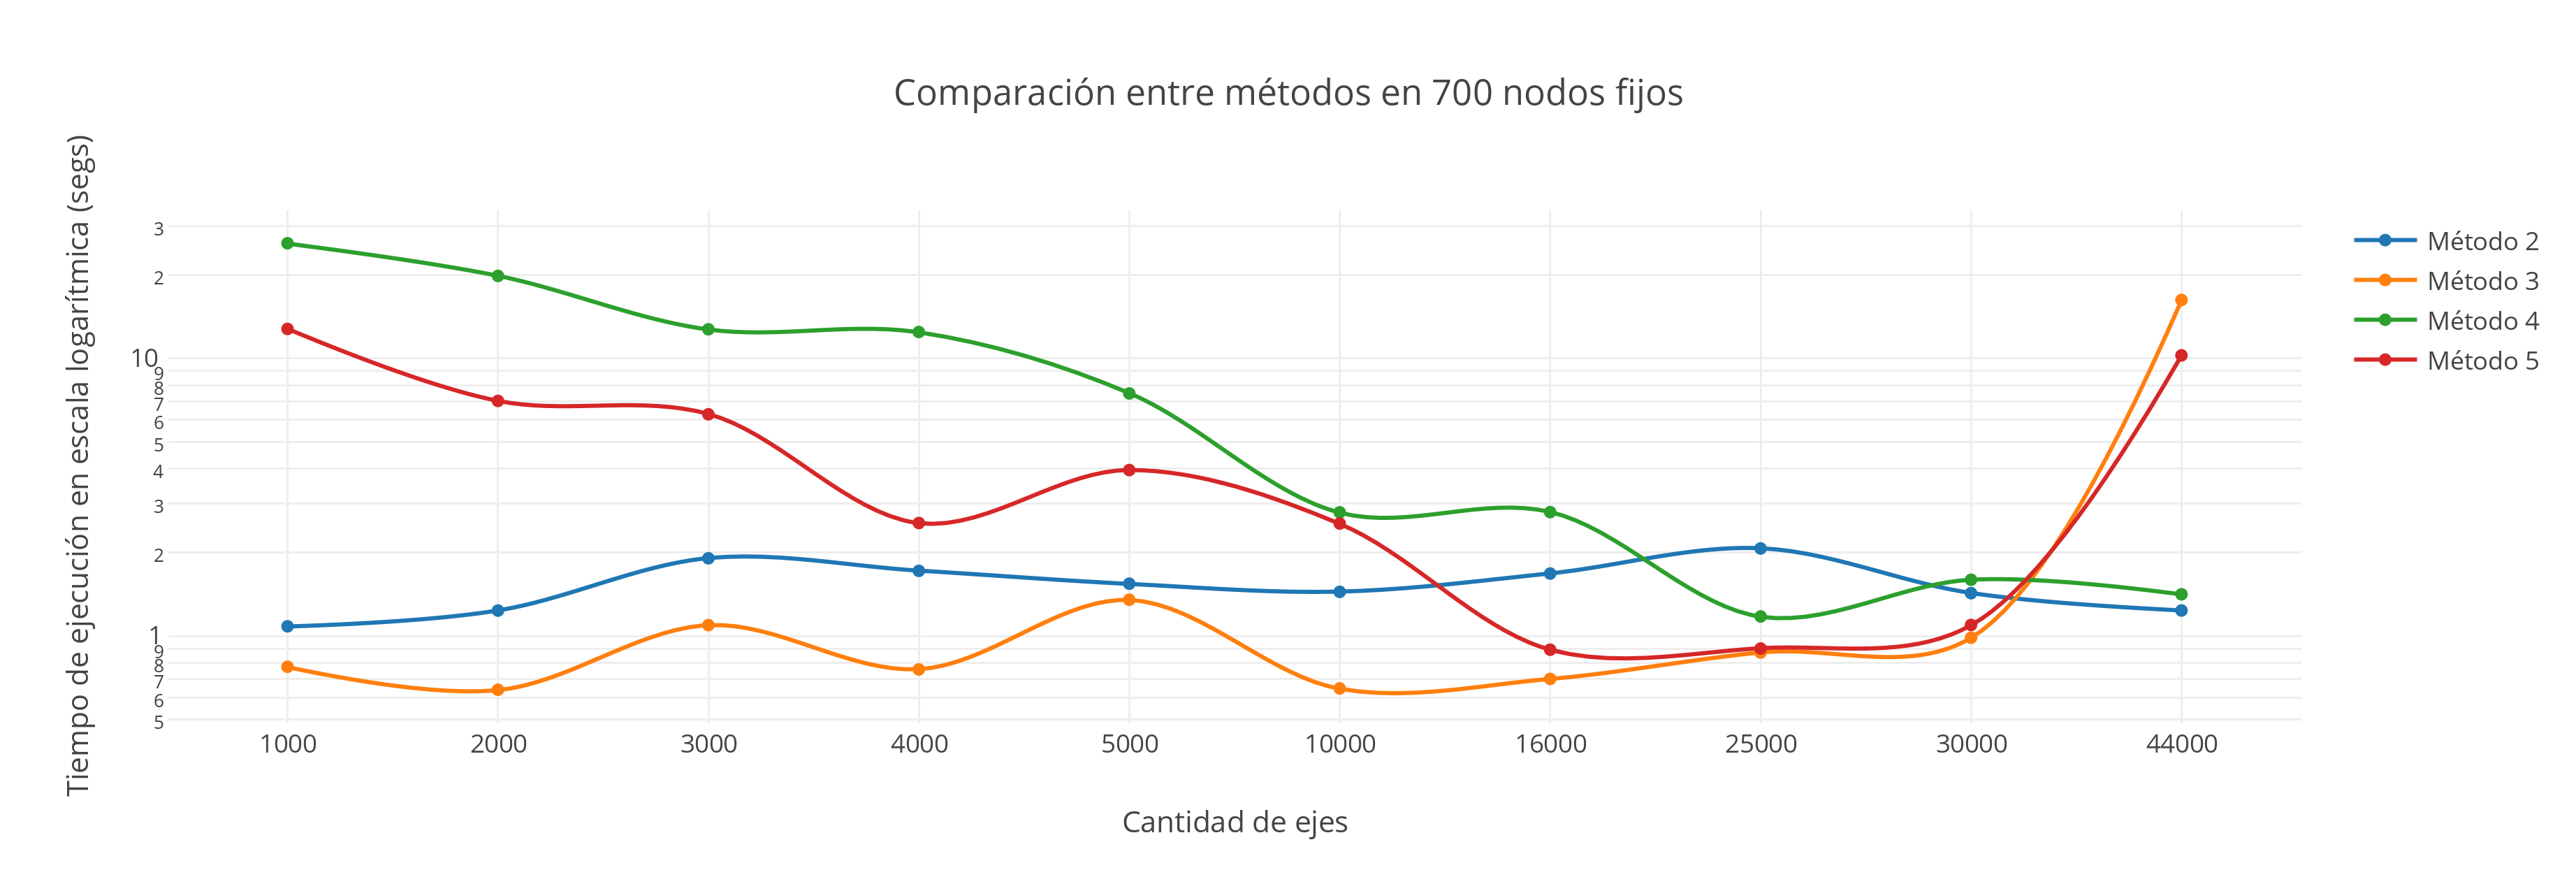
\includegraphics[scale=0.55]{imagenes/local/tiempos/700nodos.png}
% 	\caption{}
%	\label{10Nodos}
   \end{center}
 \end{figure} 
 
   \begin{figure}[h!]
   \begin{center}
 	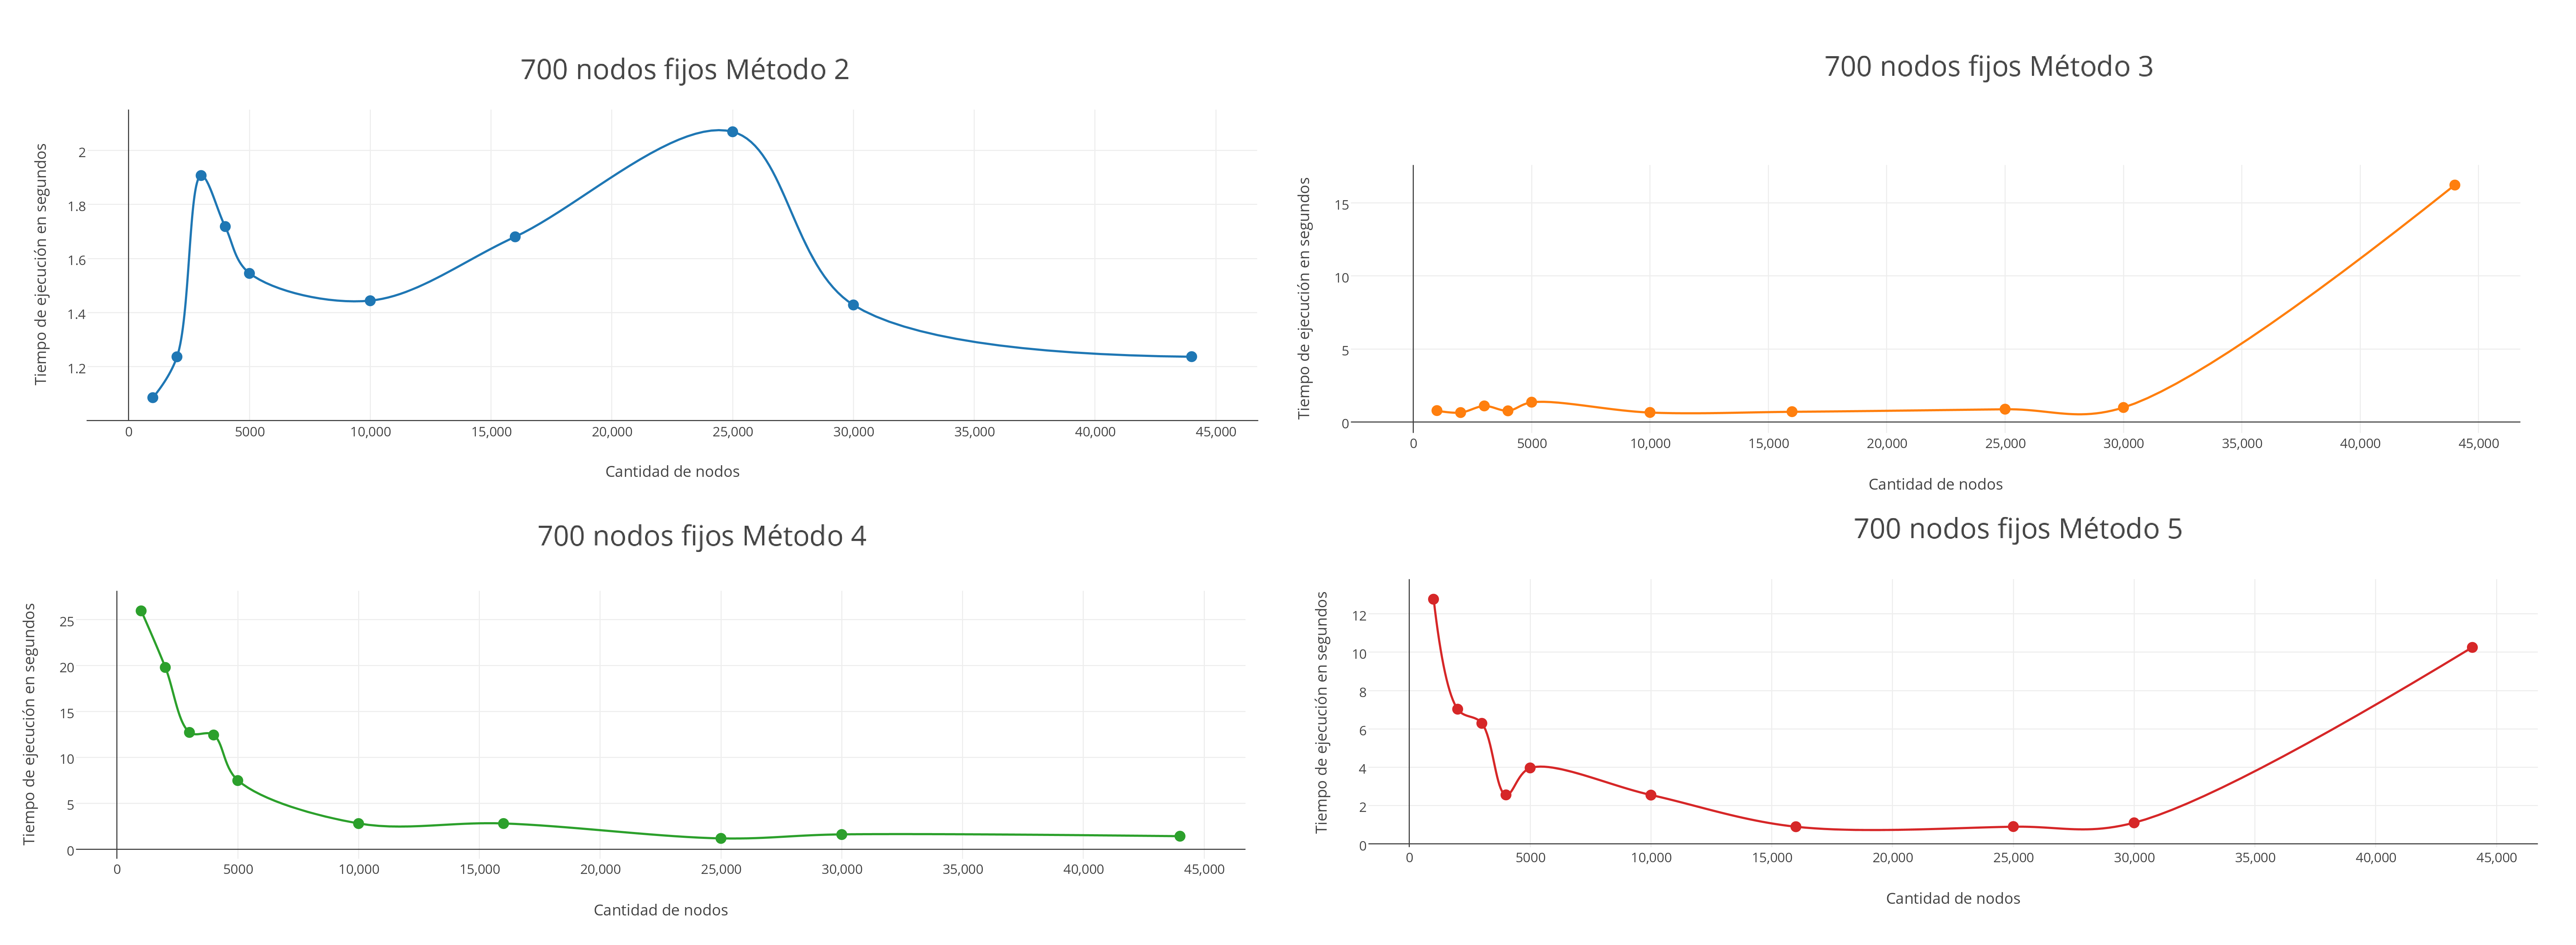
\includegraphics[scale=0.08]{imagenes/local/tiempos/700nodos2.png}
% 	\caption{}
%	\label{10Nodos}
   \end{center}
 \end{figure} 
 
Nos pareci\'o un caso notable de distinci\'on el de 700 nodos fijos, cuando se analizan los m\'etodos por separado. 

Si bien a ciencia cierta no se puede asignar a qu\'e funci\'on pertenece cada curva, pero se pueden notar las \textcolor{red}{ra\'ices (?} que poseen las curvas. De modo que se aprecia un comportamiento no estrictamente creciente. 

 \newpage
\subsubsection{Contrastaci\'on emp\'irica de la complejidad}

Se quiso linealizar los tiempos de ejecuci\'on con el fin de poder contrastar de manera \'optima las complejidades emp\'iricas con las te\'oricas. Sin embargo, esto no fue posible debido a que los tiempos de ejecuci\'on son muy peque\~nos y al dividirlos por la cantidad de nodos los resultados obtenidos no generan gr\'aficos de real inter\'es.\\

A continuaci\'on se exponen los tiempos de ejecuci\'on para los distintos m\'etodos, considerando grafos Ciclo y grafos Completos:

  \begin{figure}[h!]
   \begin{center}
 	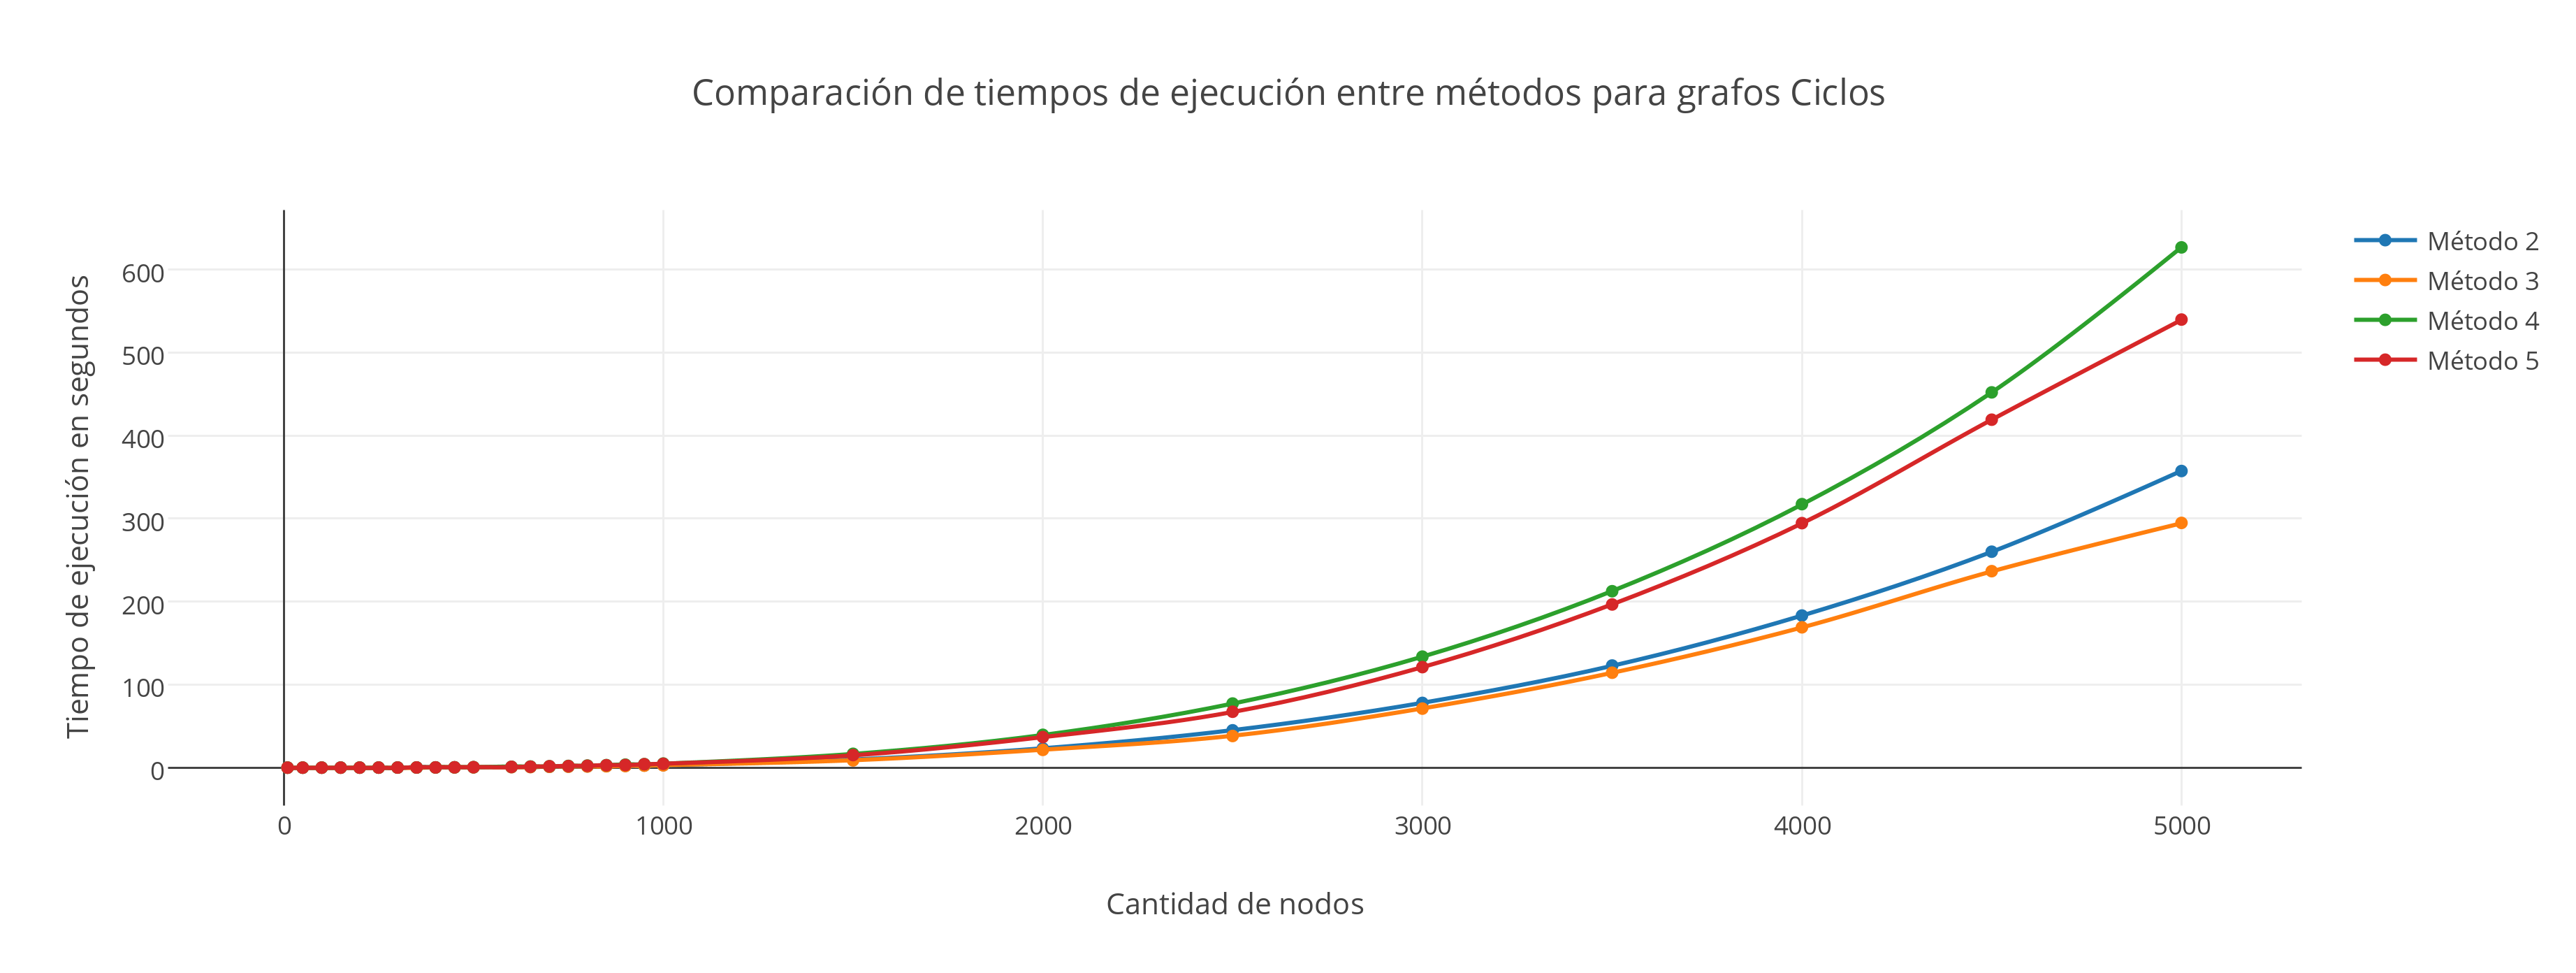
\includegraphics[scale=0.55]{imagenes/local/tiempos/ciclos.png}
% 	\caption{}
%	\label{10Nodos}
   \end{center}
 \end{figure} 
 
Los tiempos de ejecuci\'on para grafos Ciclos se condicen con los gr\'aficos de la secci\'on \ref{tiempos}. Esto significa que los \textbf{m\'etodos 4} y \textbf{5} poseen mayor tiempo de ejecuci\'on y finalmente, el \textbf{m\'etodo 2} preserva el menor.

Todas las curvas presentan un comportamiento que se asemeja a un valor cuadr\'atico  o c\'ubico, ya que si bien la complejidad te\'orica es de \textcolor{red}{$O(n^5)$ (?)} al tener s\'olo dos vecinos cada nodo las listas de adyacencia se recorren en $O(2)\subseteq O(1)$.
 
   \begin{figure}[h!]
   \begin{center}
 	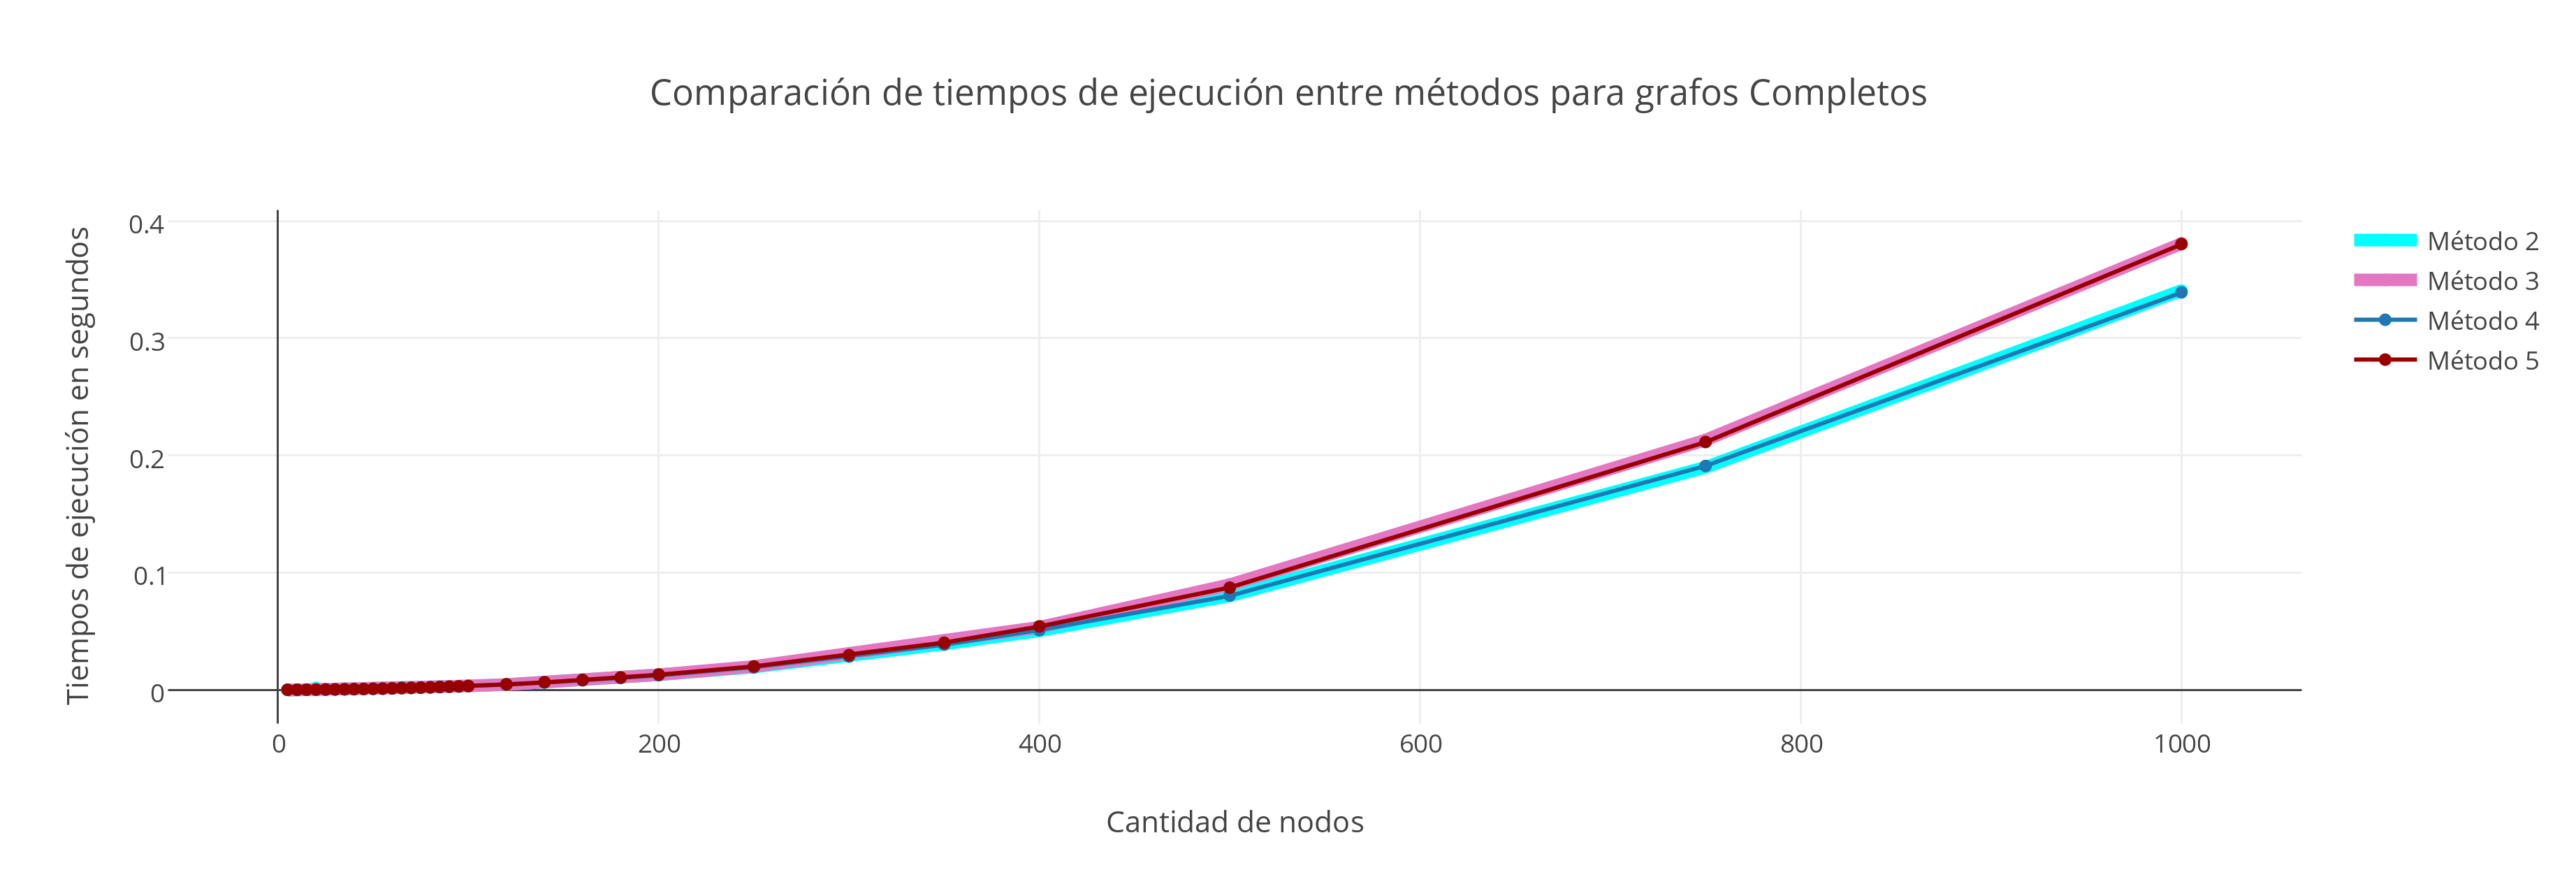
\includegraphics[scale=0.55]{imagenes/local/tiempos/completos.png}
% 	\caption{}
%	\label{10Nodos}
   \end{center}
 \end{figure} 
 
\textcolor{red}{Los grafos completos son... } 
 
\newpage
\subsubsection{Comparaci\'on soluciones Local vs Exacto}

  \begin{figure}[h!]
   \begin{center}
 	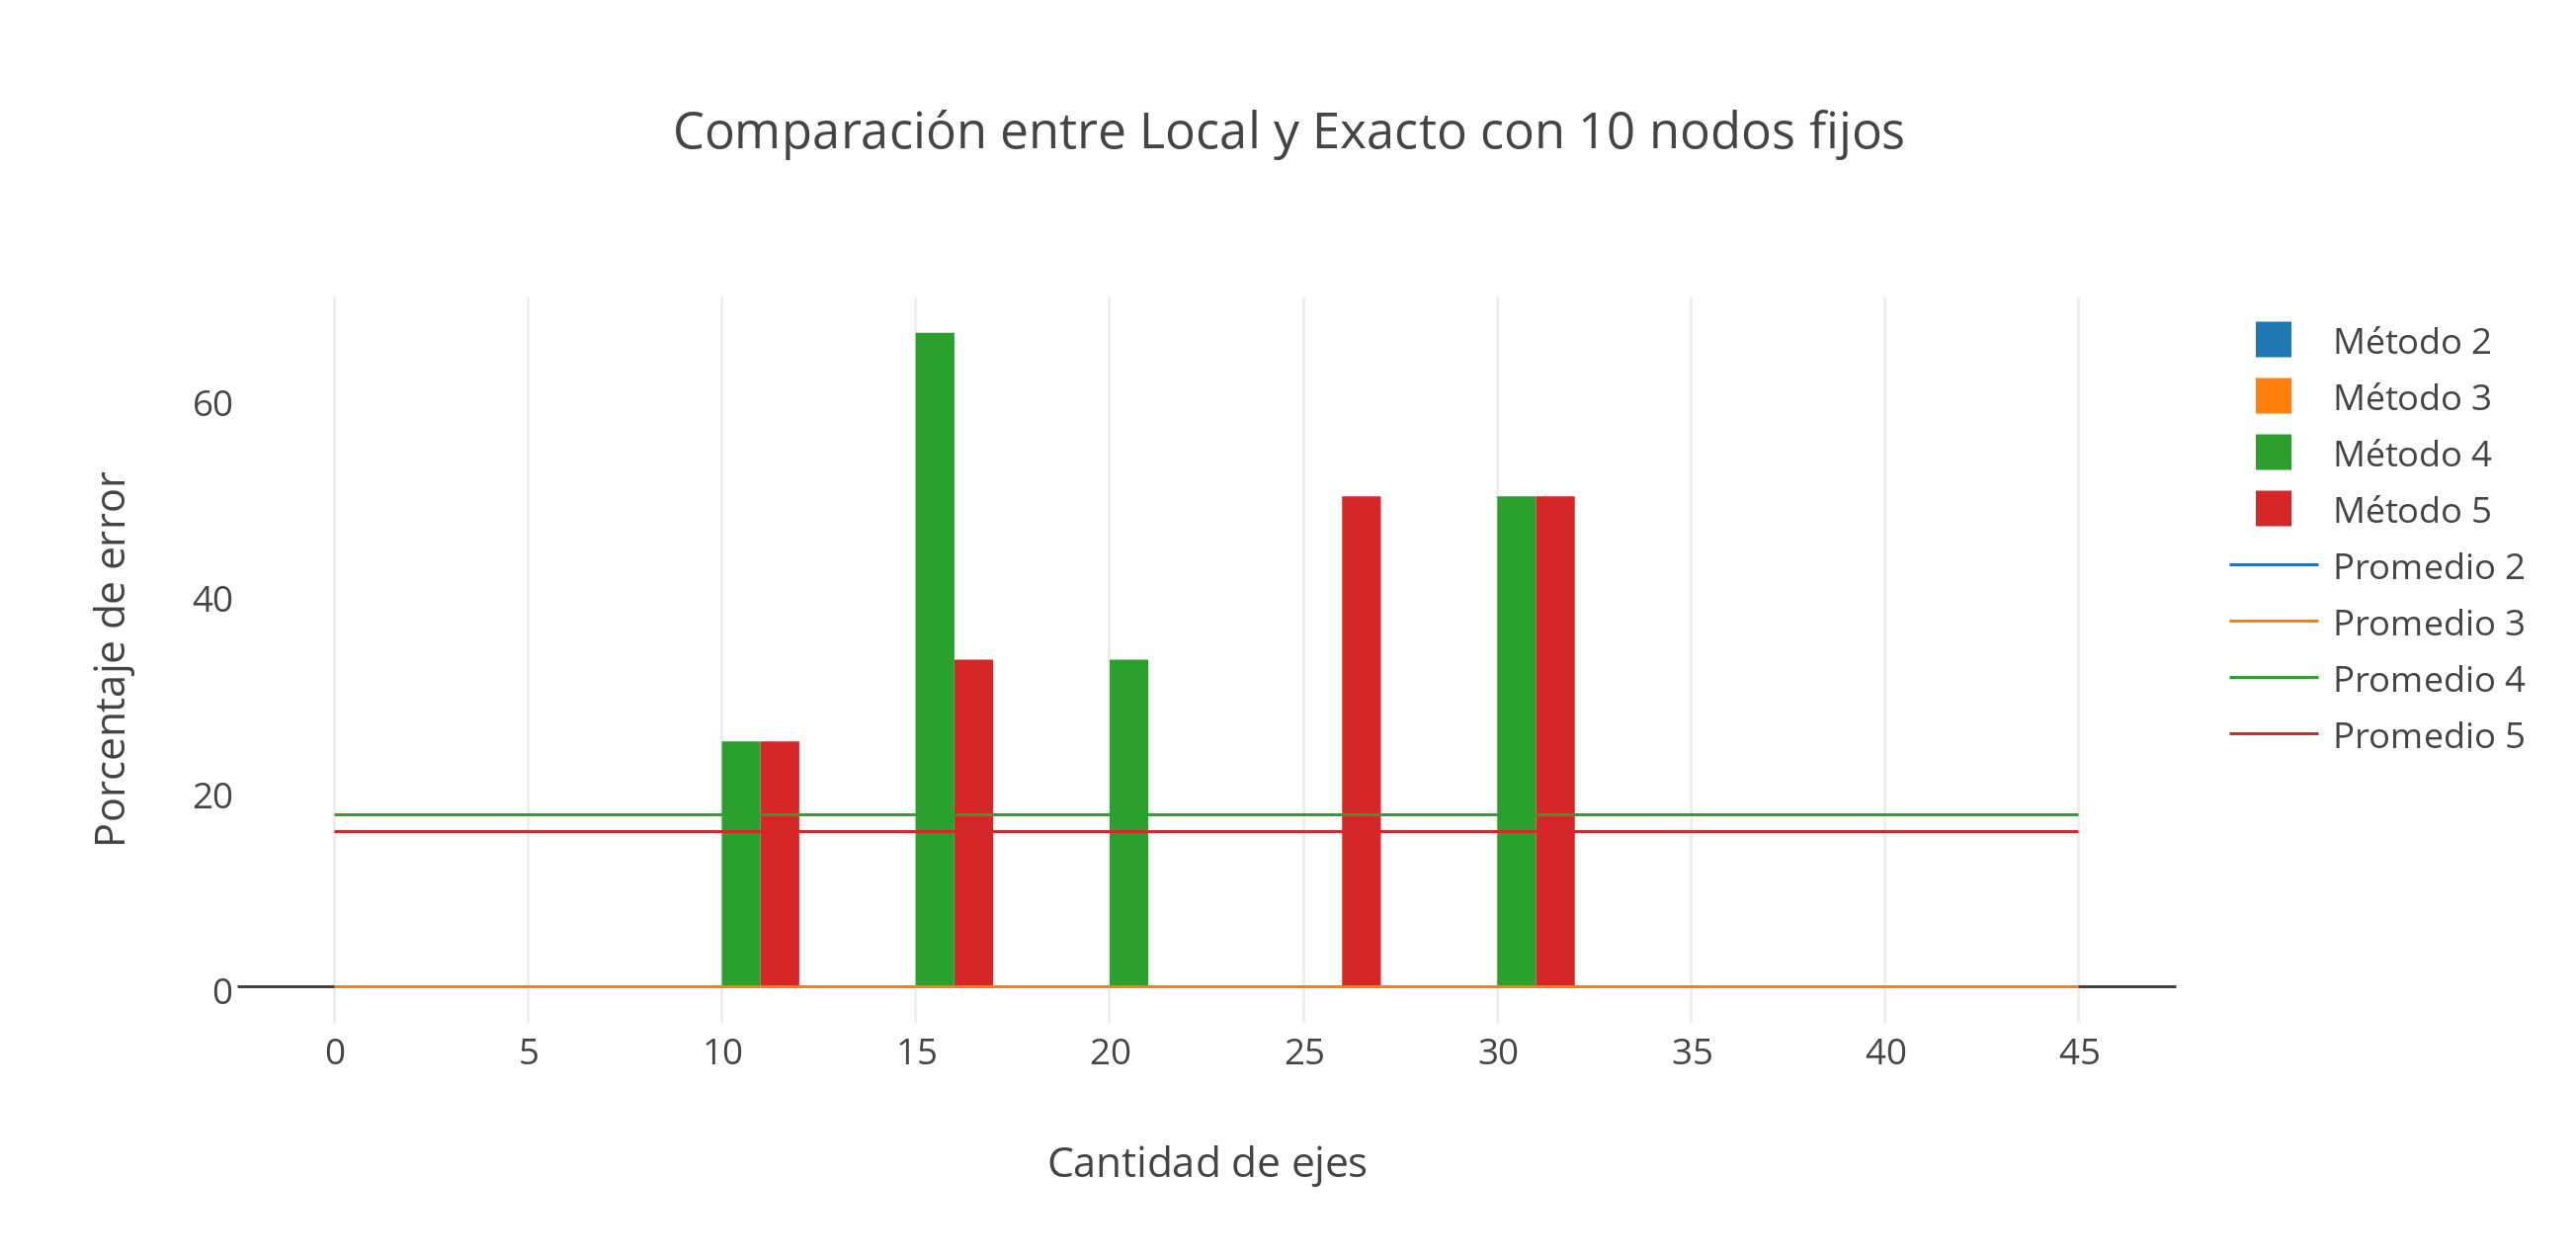
\includegraphics[scale=0.75]{imagenes/local/exacto/10nodos.png}
% 	\caption{}
%	\label{10Nodos}
   \end{center}
 \end{figure}

  \begin{figure}[h!]
   \begin{center}
 	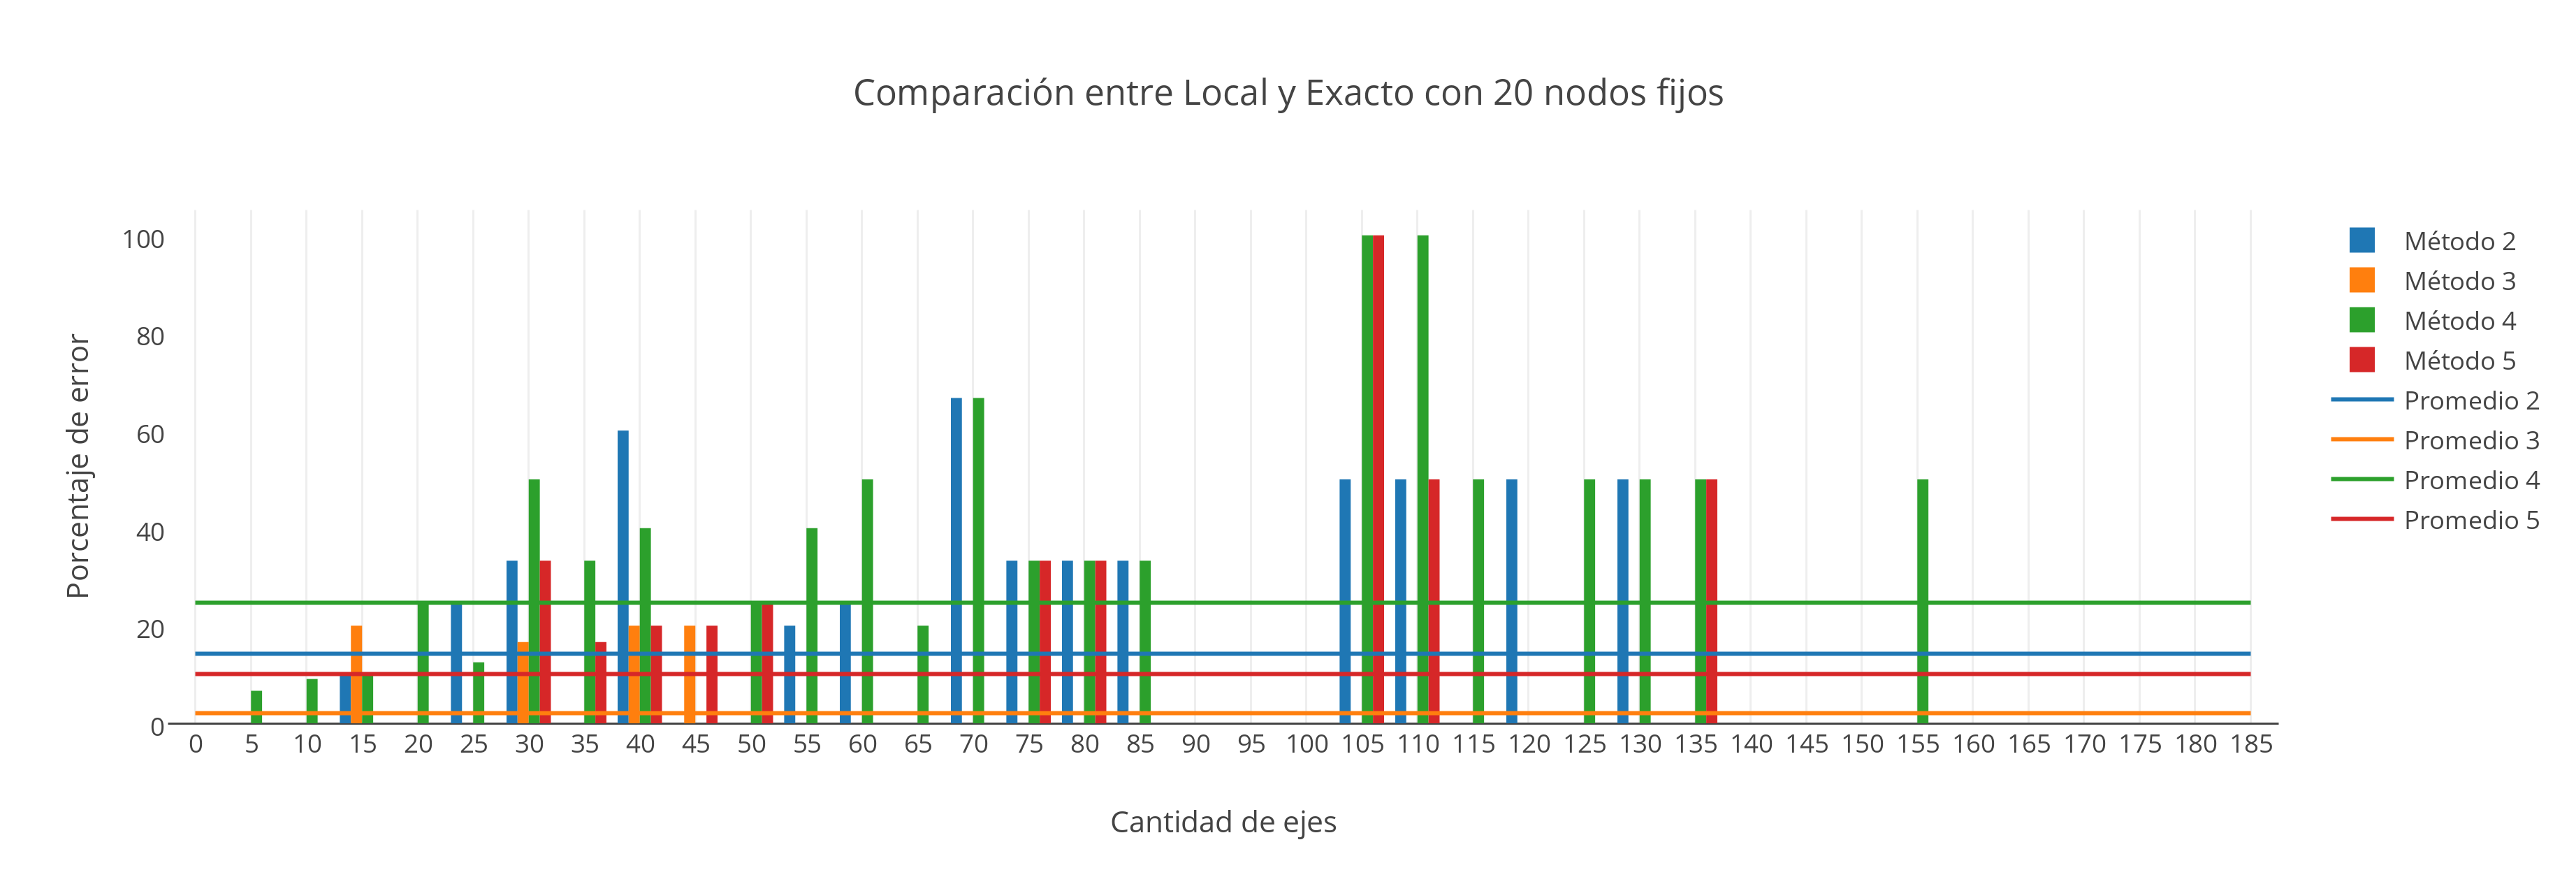
\includegraphics[scale=0.55]{imagenes/local/exacto/20nodos.png}
% 	\caption{}
%	\label{10Nodos}
   \end{center}
 \end{figure}
 
   \begin{figure}[h!]
   \begin{center}
 	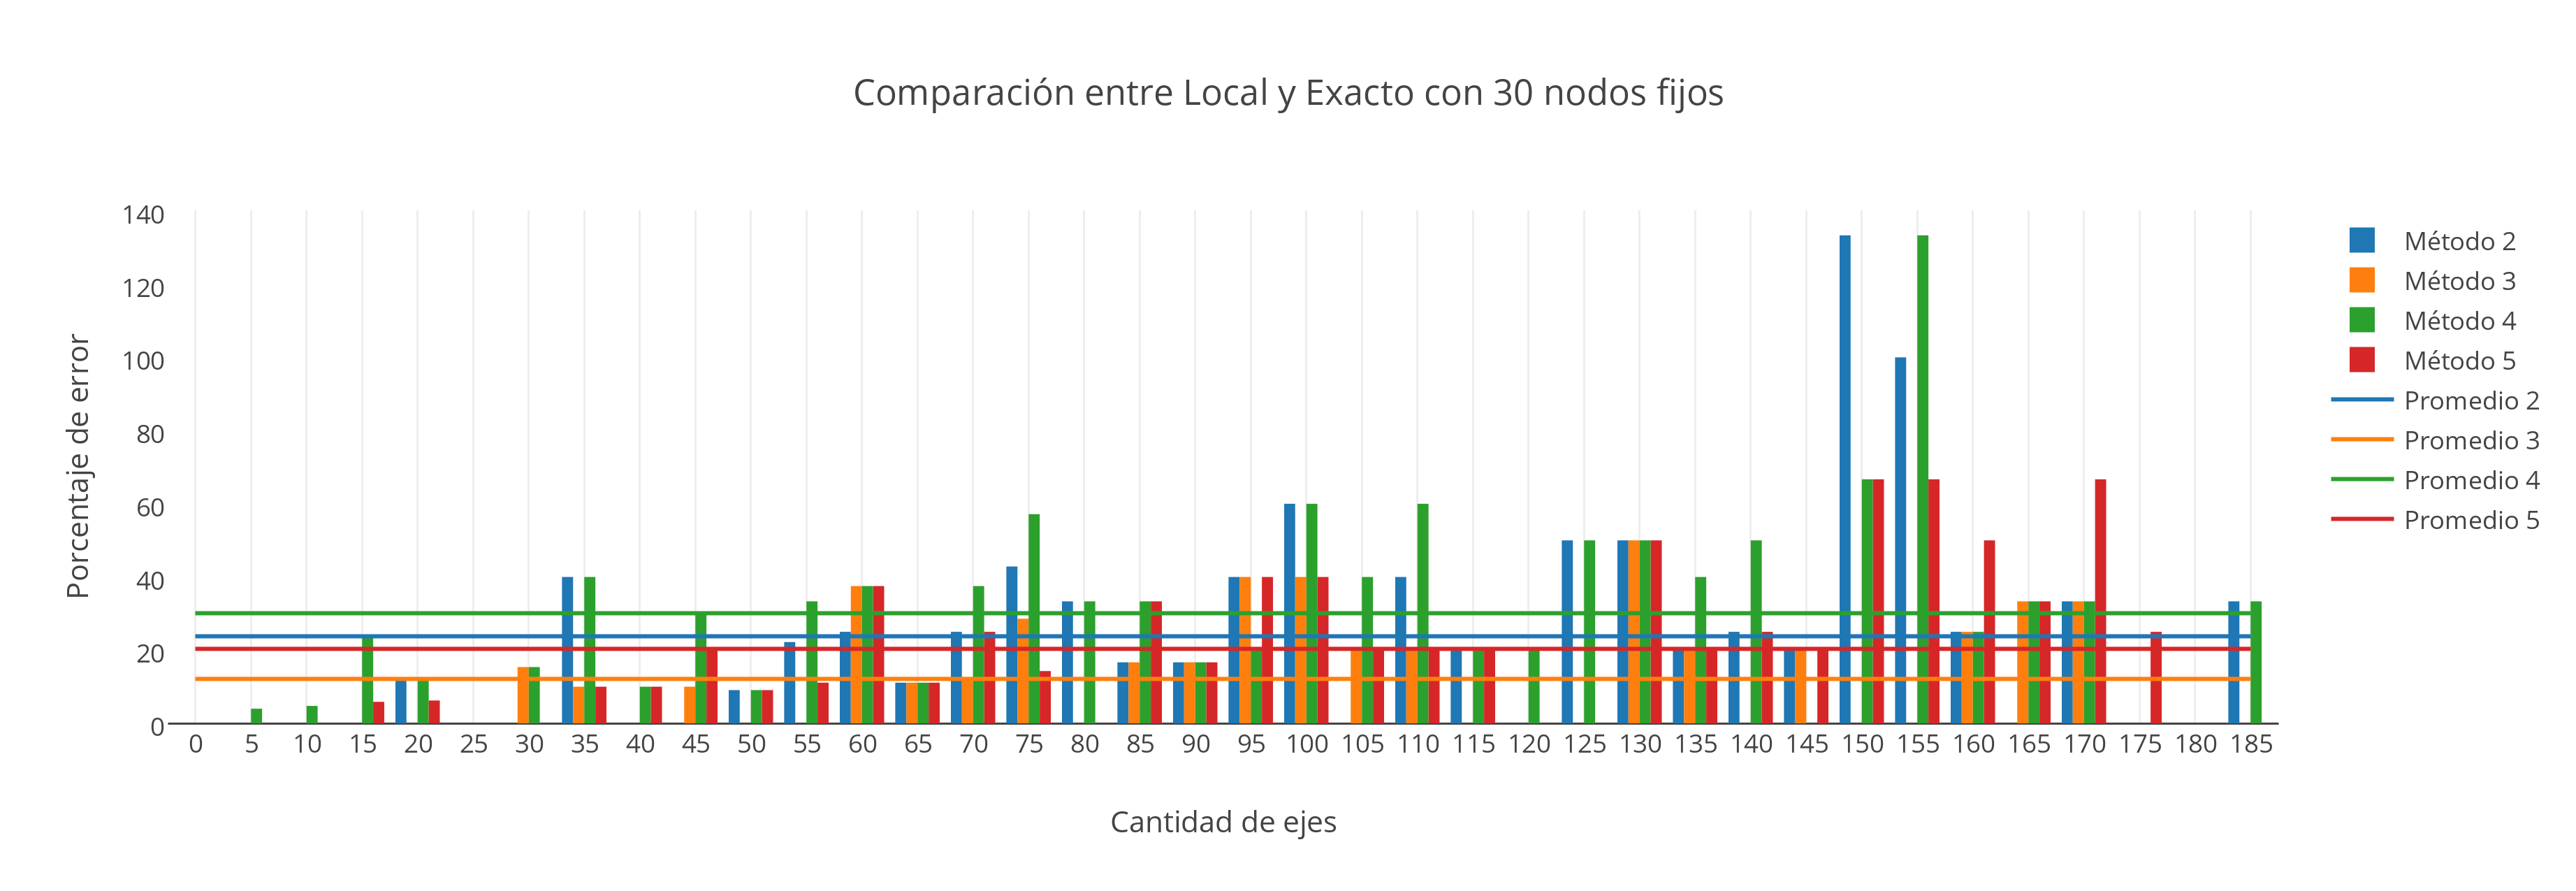
\includegraphics[scale=0.55]{imagenes/local/exacto/30nodos.png}
% 	\caption{}
%	\label{10Nodos}
   \end{center}
 \end{figure}

\newpage

  \begin{figure}[h!]
   \begin{center}
 	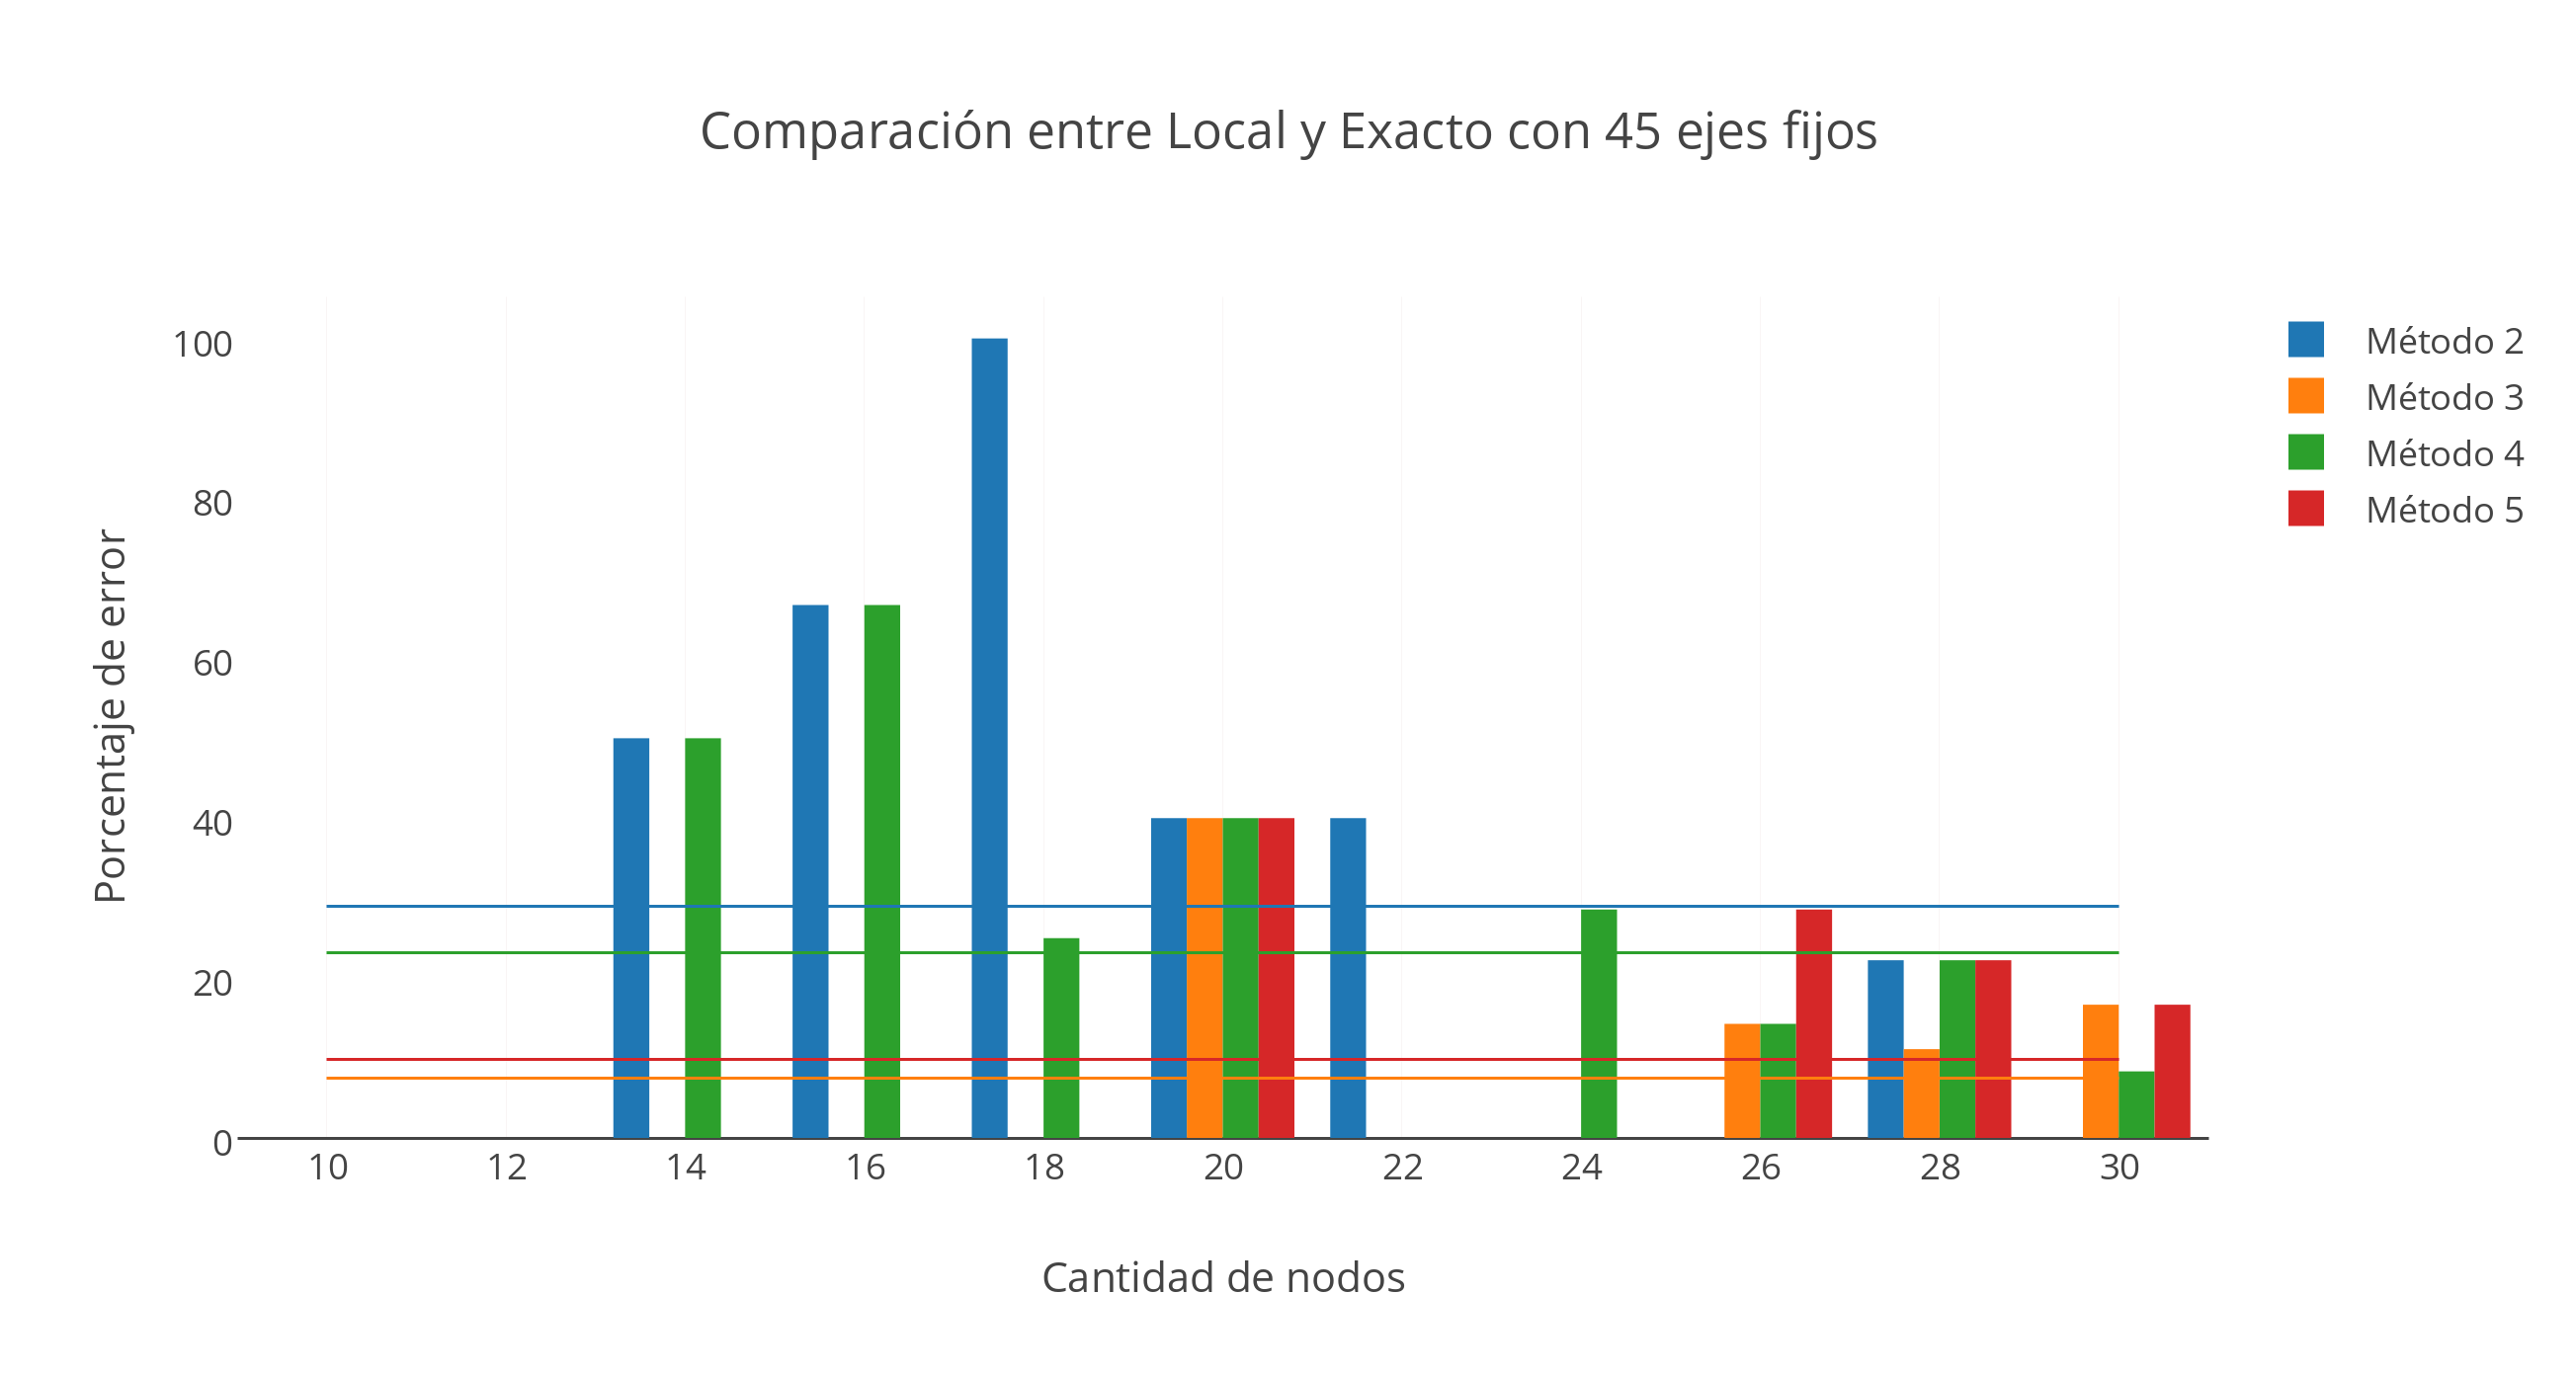
\includegraphics[scale=0.7]{imagenes/local/exacto/45ejes.png}
% 	\caption{}
%	\label{10Nodos}
   \end{center}
 \end{figure} 
 
  \begin{figure}[h!]
   \begin{center}
 	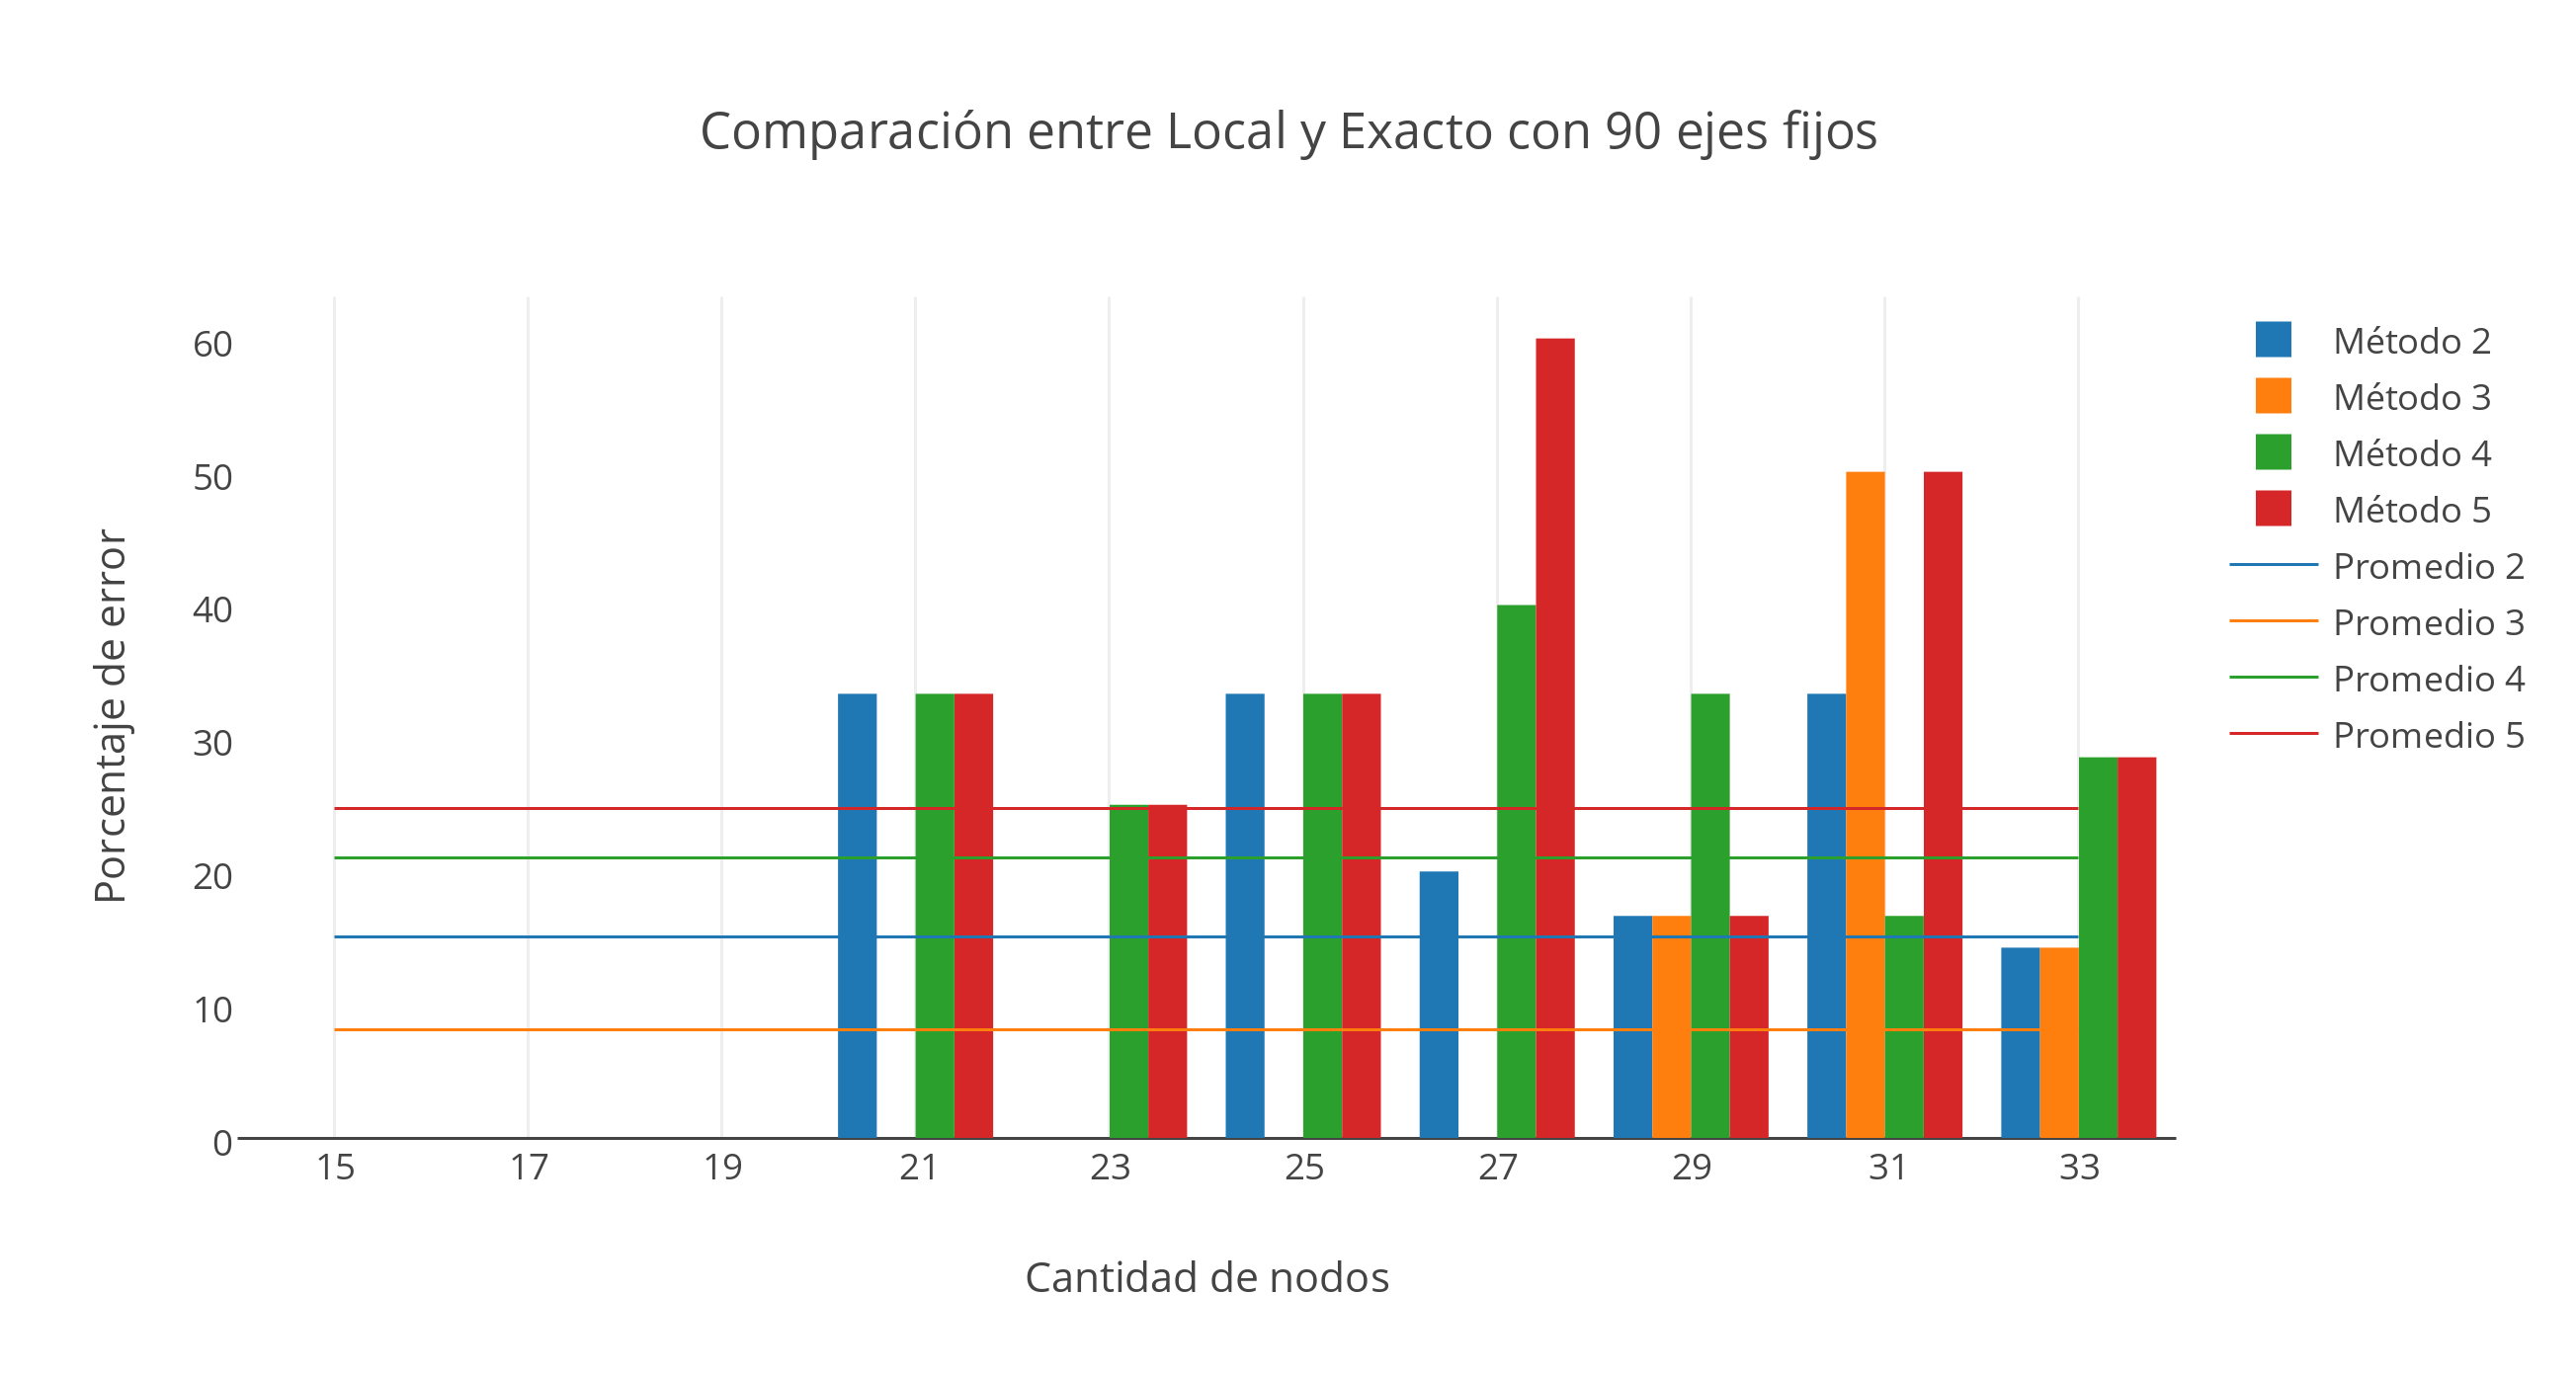
\includegraphics[scale=0.7]{imagenes/local/exacto/90ejes.png}
% 	\caption{}
%	\label{10Nodos}
   \end{center}
 \end{figure} 
 
 \newpage
  \begin{figure}[h!]
   \begin{center}
 	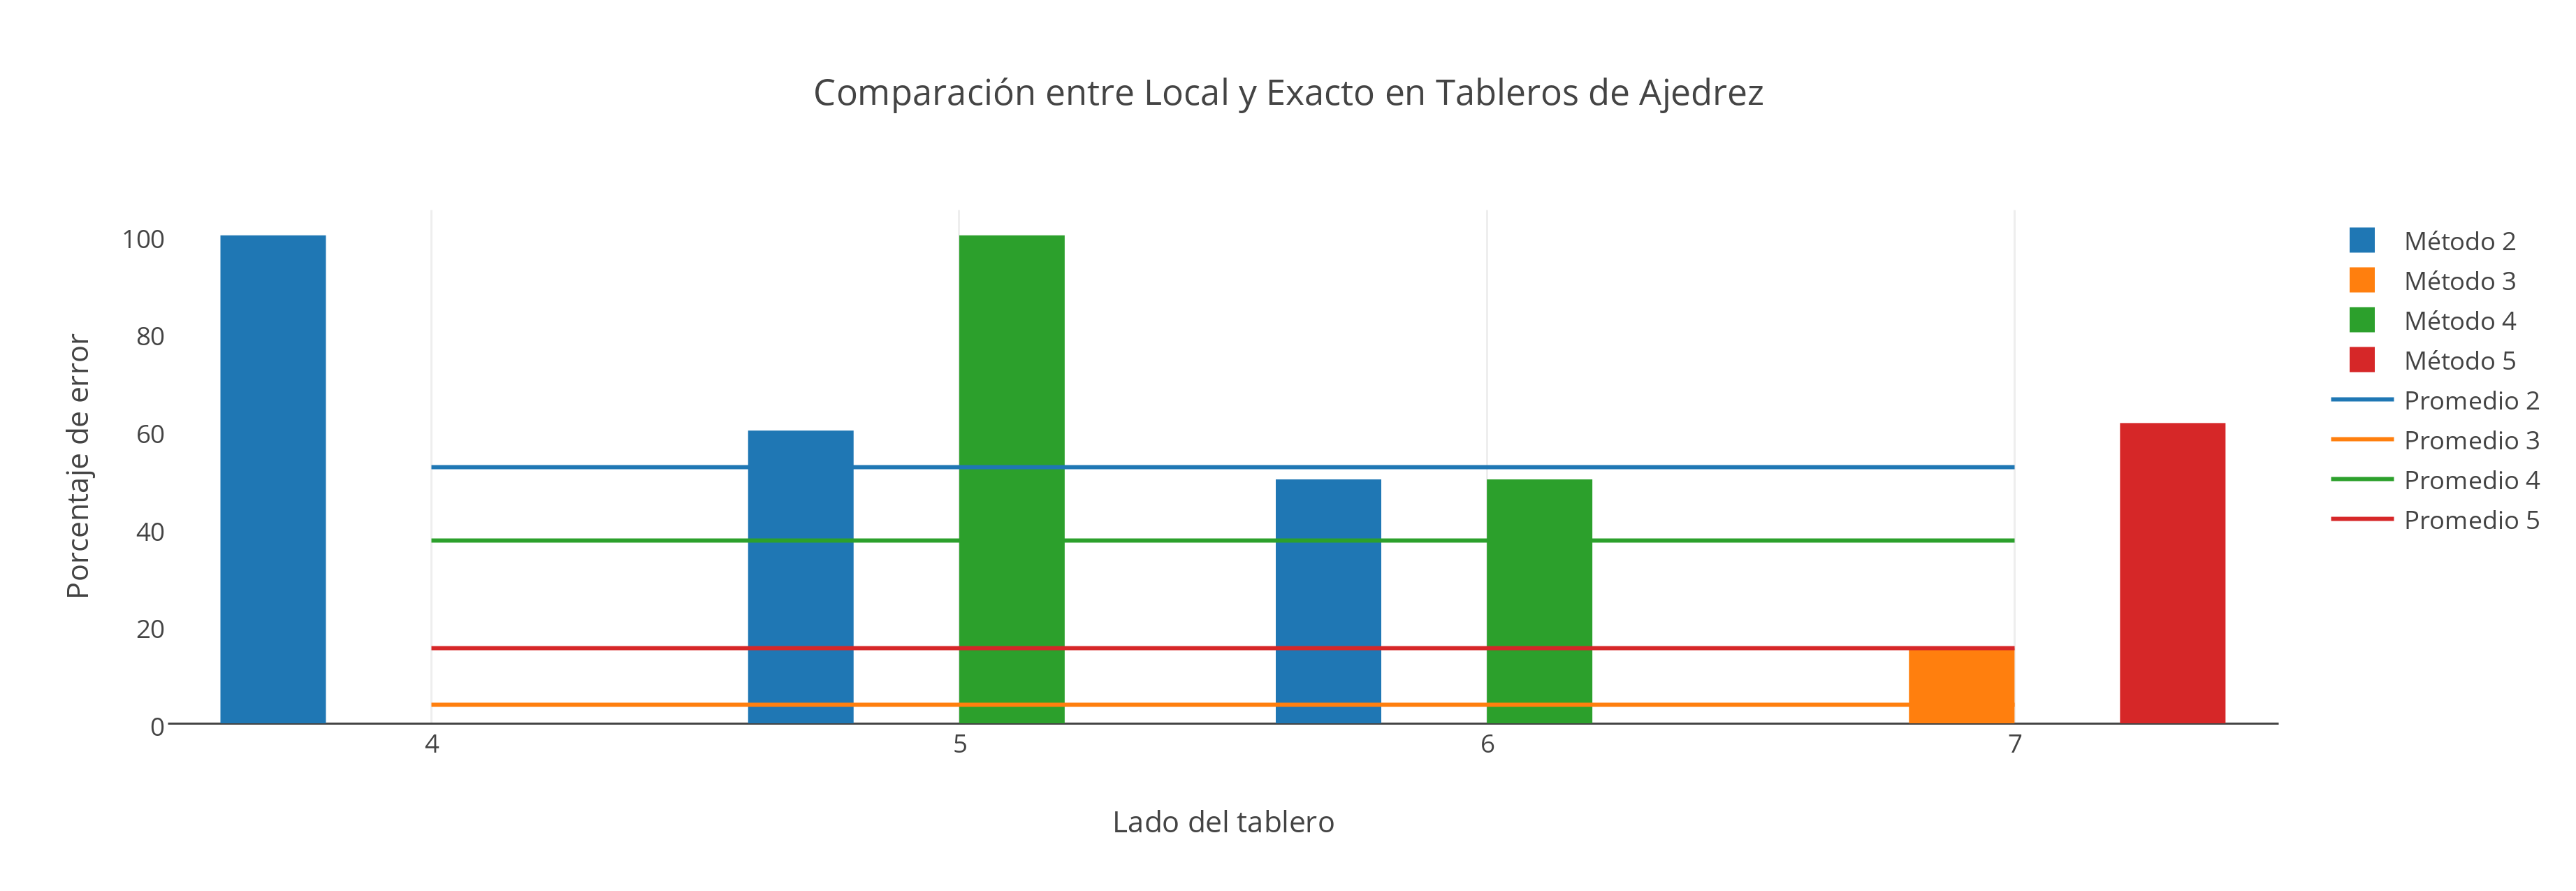
\includegraphics[scale=0.55]{imagenes/local/exacto/tableros.png}
% 	\caption{}
%	\label{10Nodos}
   \end{center}
 \end{figure} 
 
\newpage 
 
\subsubsection{Elecci\'on de versi\'on \'optima}

\subsubsection*{Ejes Fijos}


  \begin{figure}[h!]
   \begin{center}
 	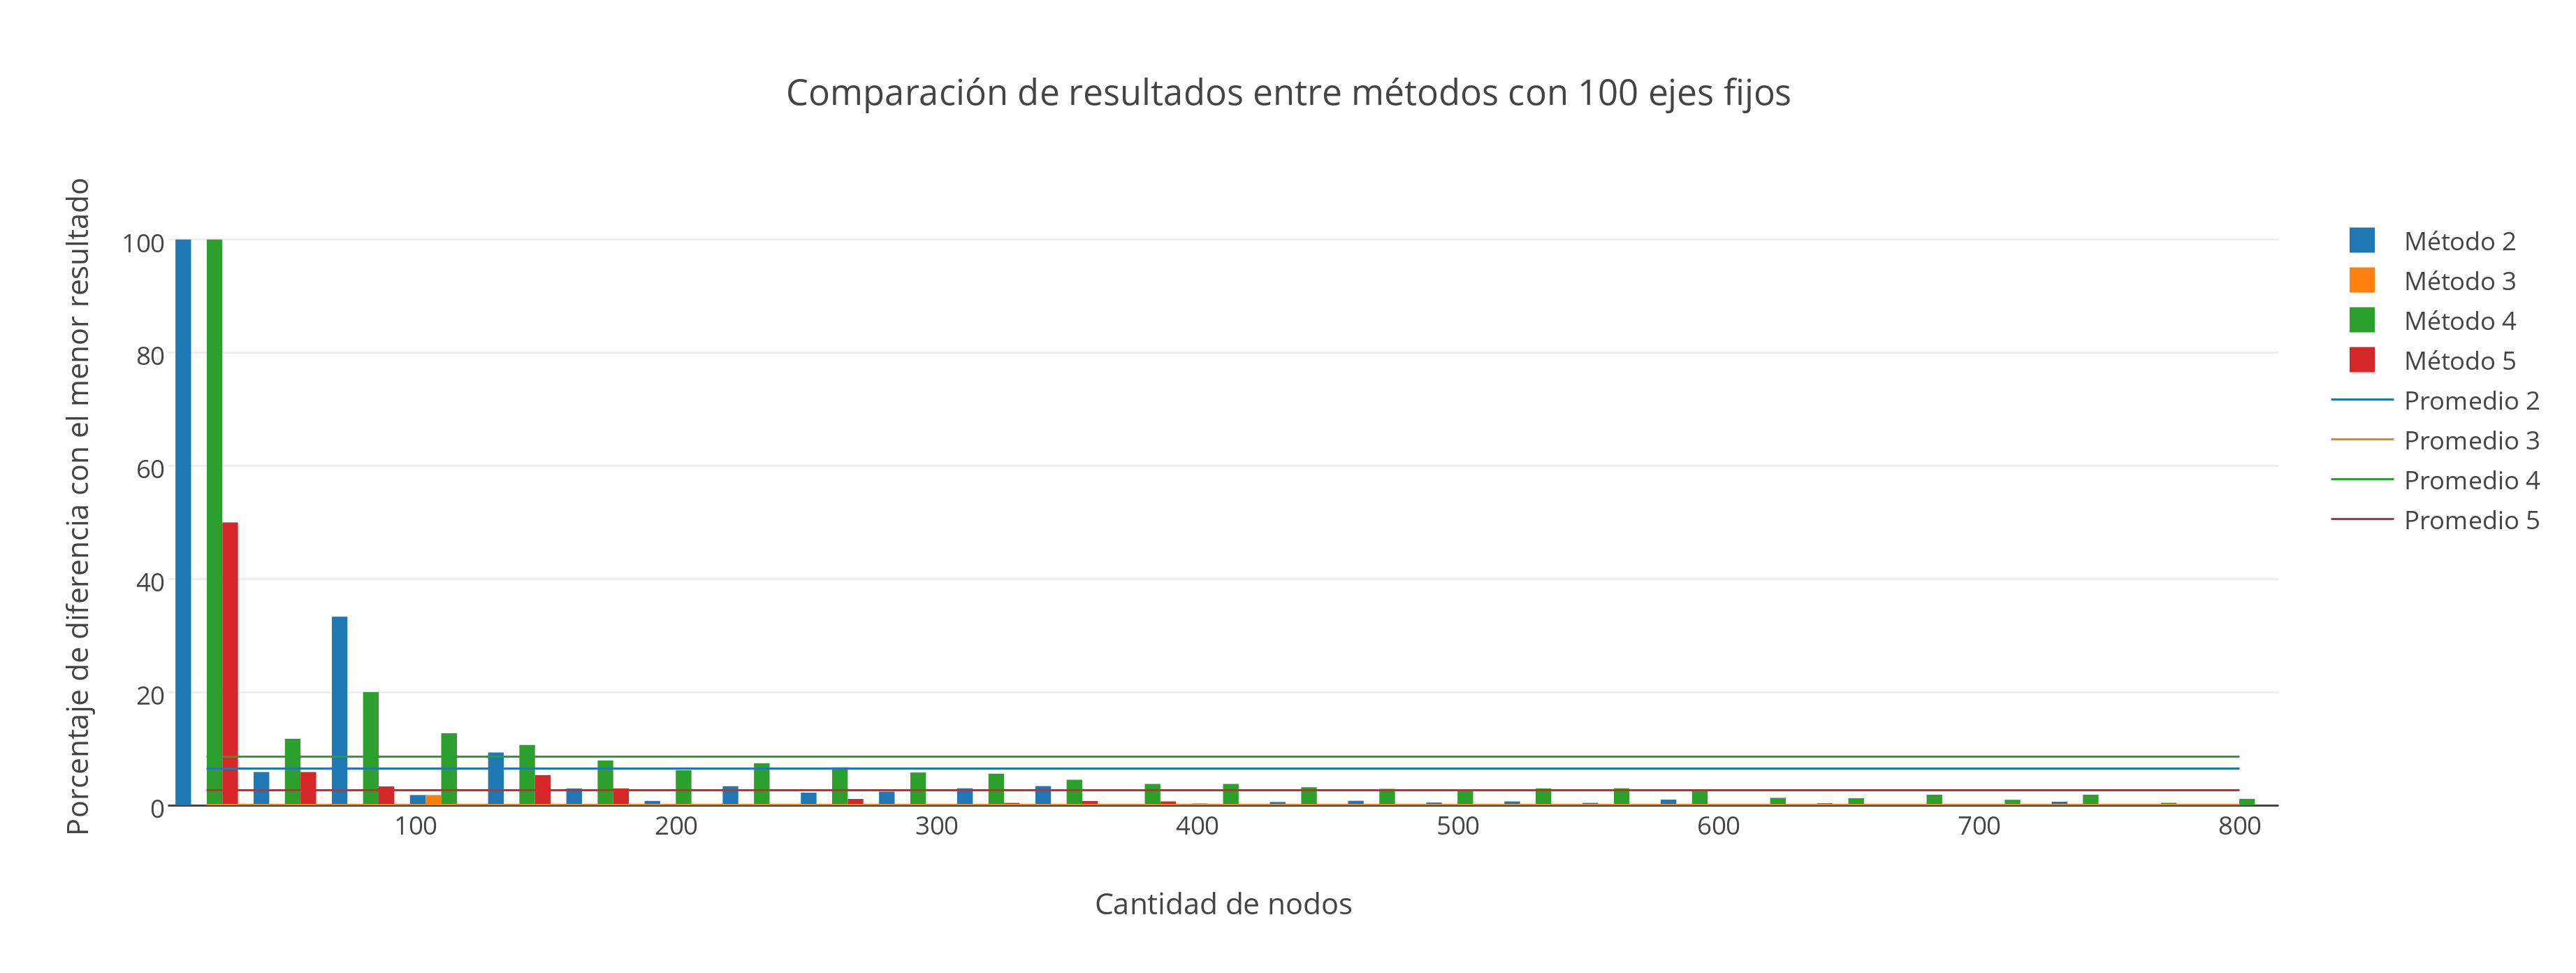
\includegraphics[scale=0.55]{imagenes/local/resultados/100ejes.png}
% 	\caption{}
%	\label{10Nodos}
   \end{center}
 \end{figure}
 

  \begin{figure}[h!]
   \begin{center}
 	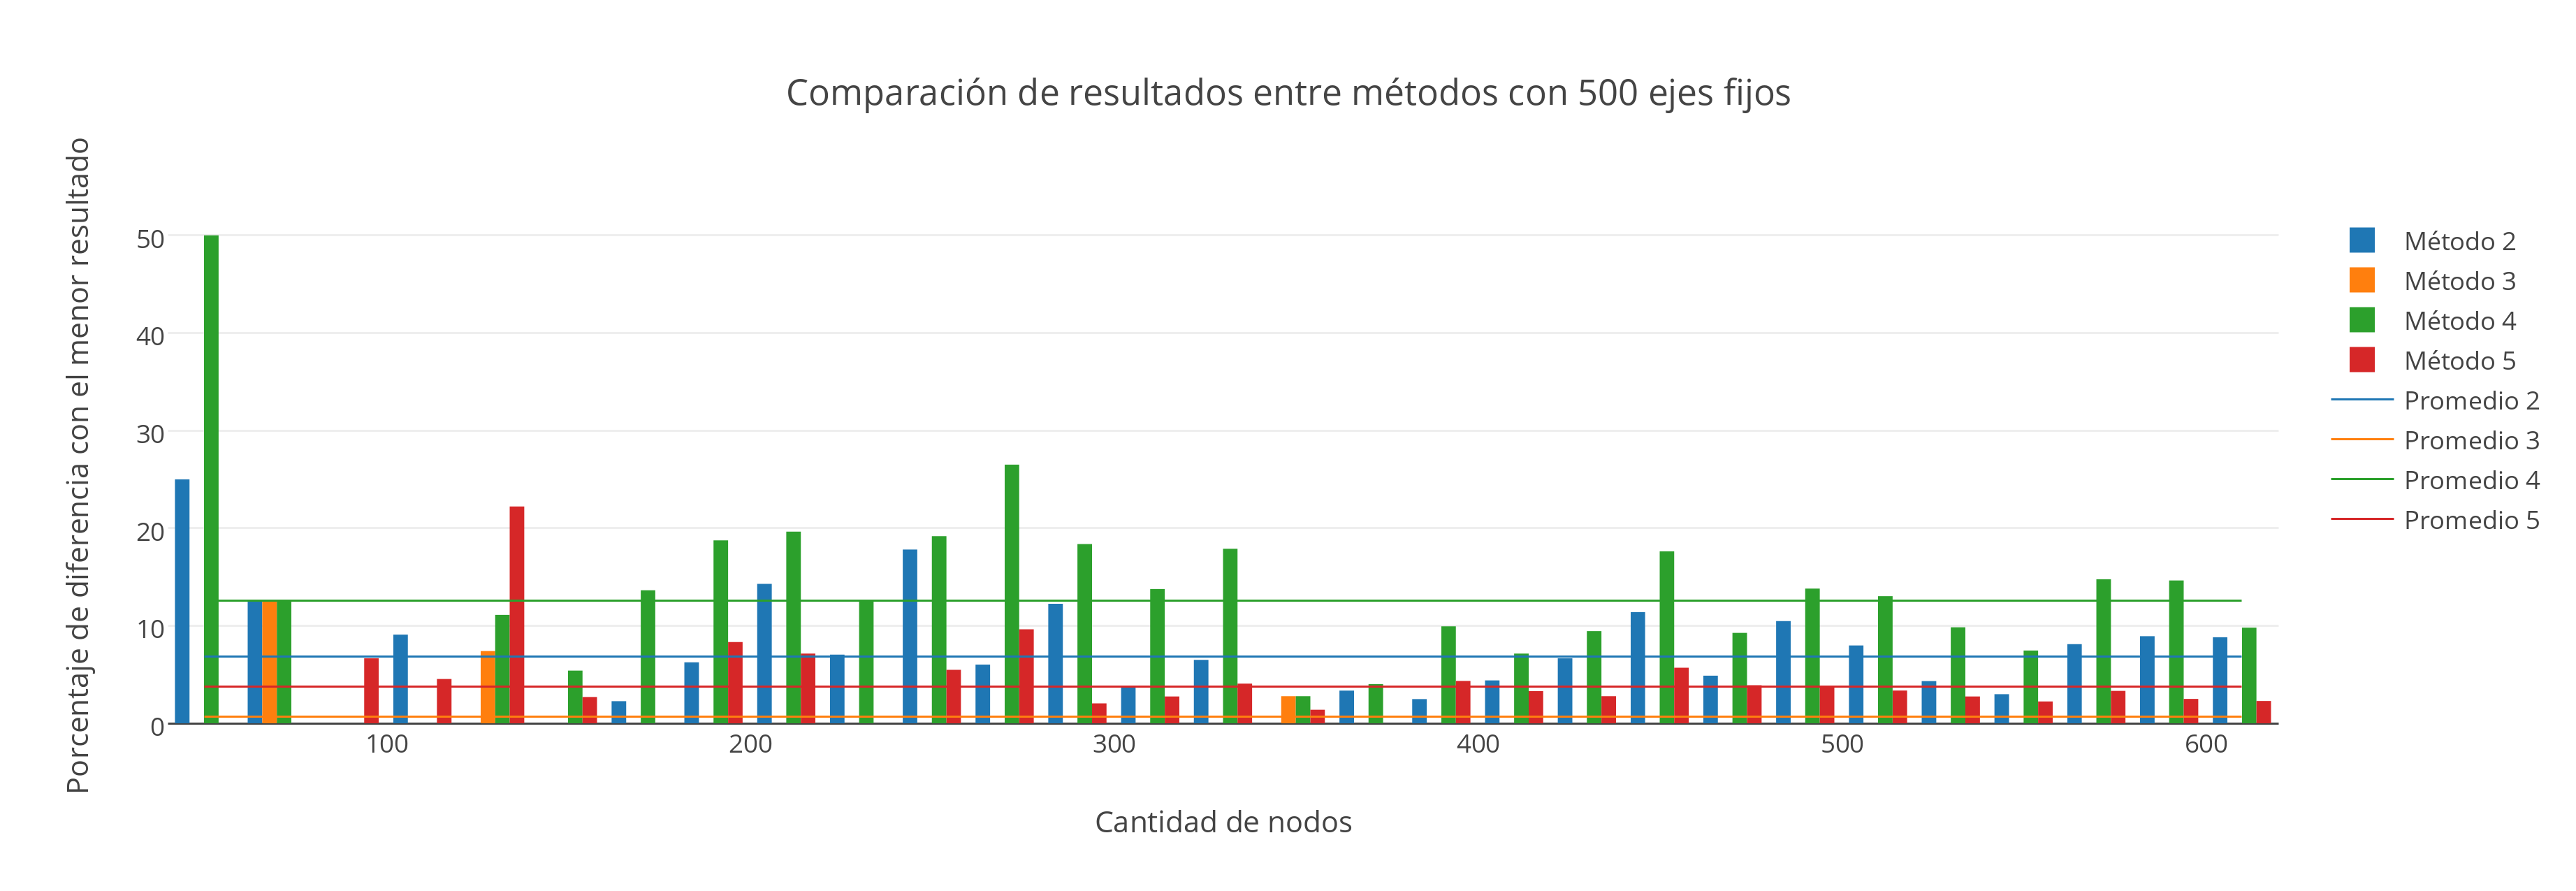
\includegraphics[scale=0.55]{imagenes/local/resultados/500ejes.png}
% 	\caption{}
%	\label{10Nodos}
   \end{center}
 \end{figure}
 
   \begin{figure}[h!]
   \begin{center}
 	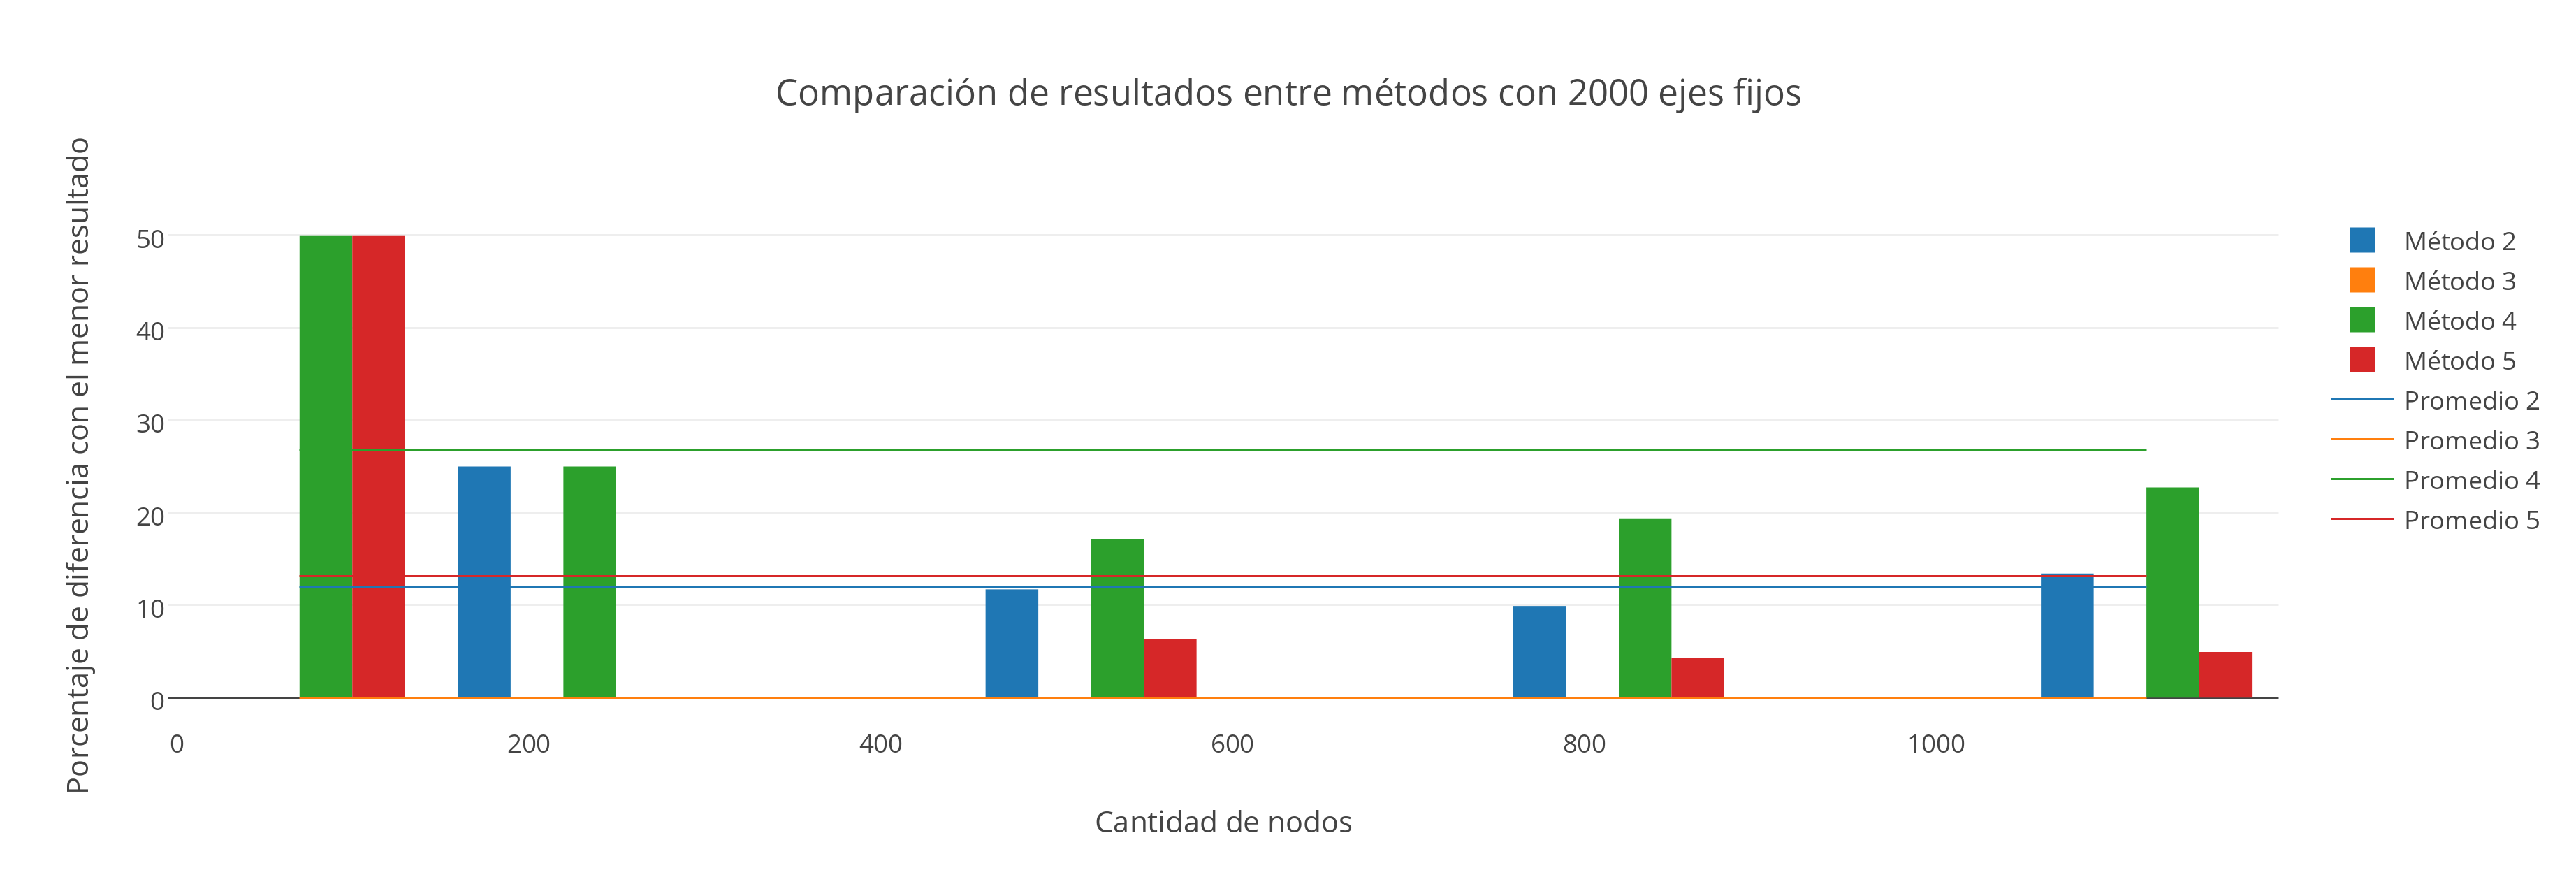
\includegraphics[scale=0.55]{imagenes/local/resultados/2000ejes.png}
% 	\caption{}
%	\label{10Nodos}
   \end{center}
 \end{figure}
 
  
\newpage  
  
\subsubsection*{Nodos Fijos}

  \begin{figure}[h!]
   \begin{center}
 	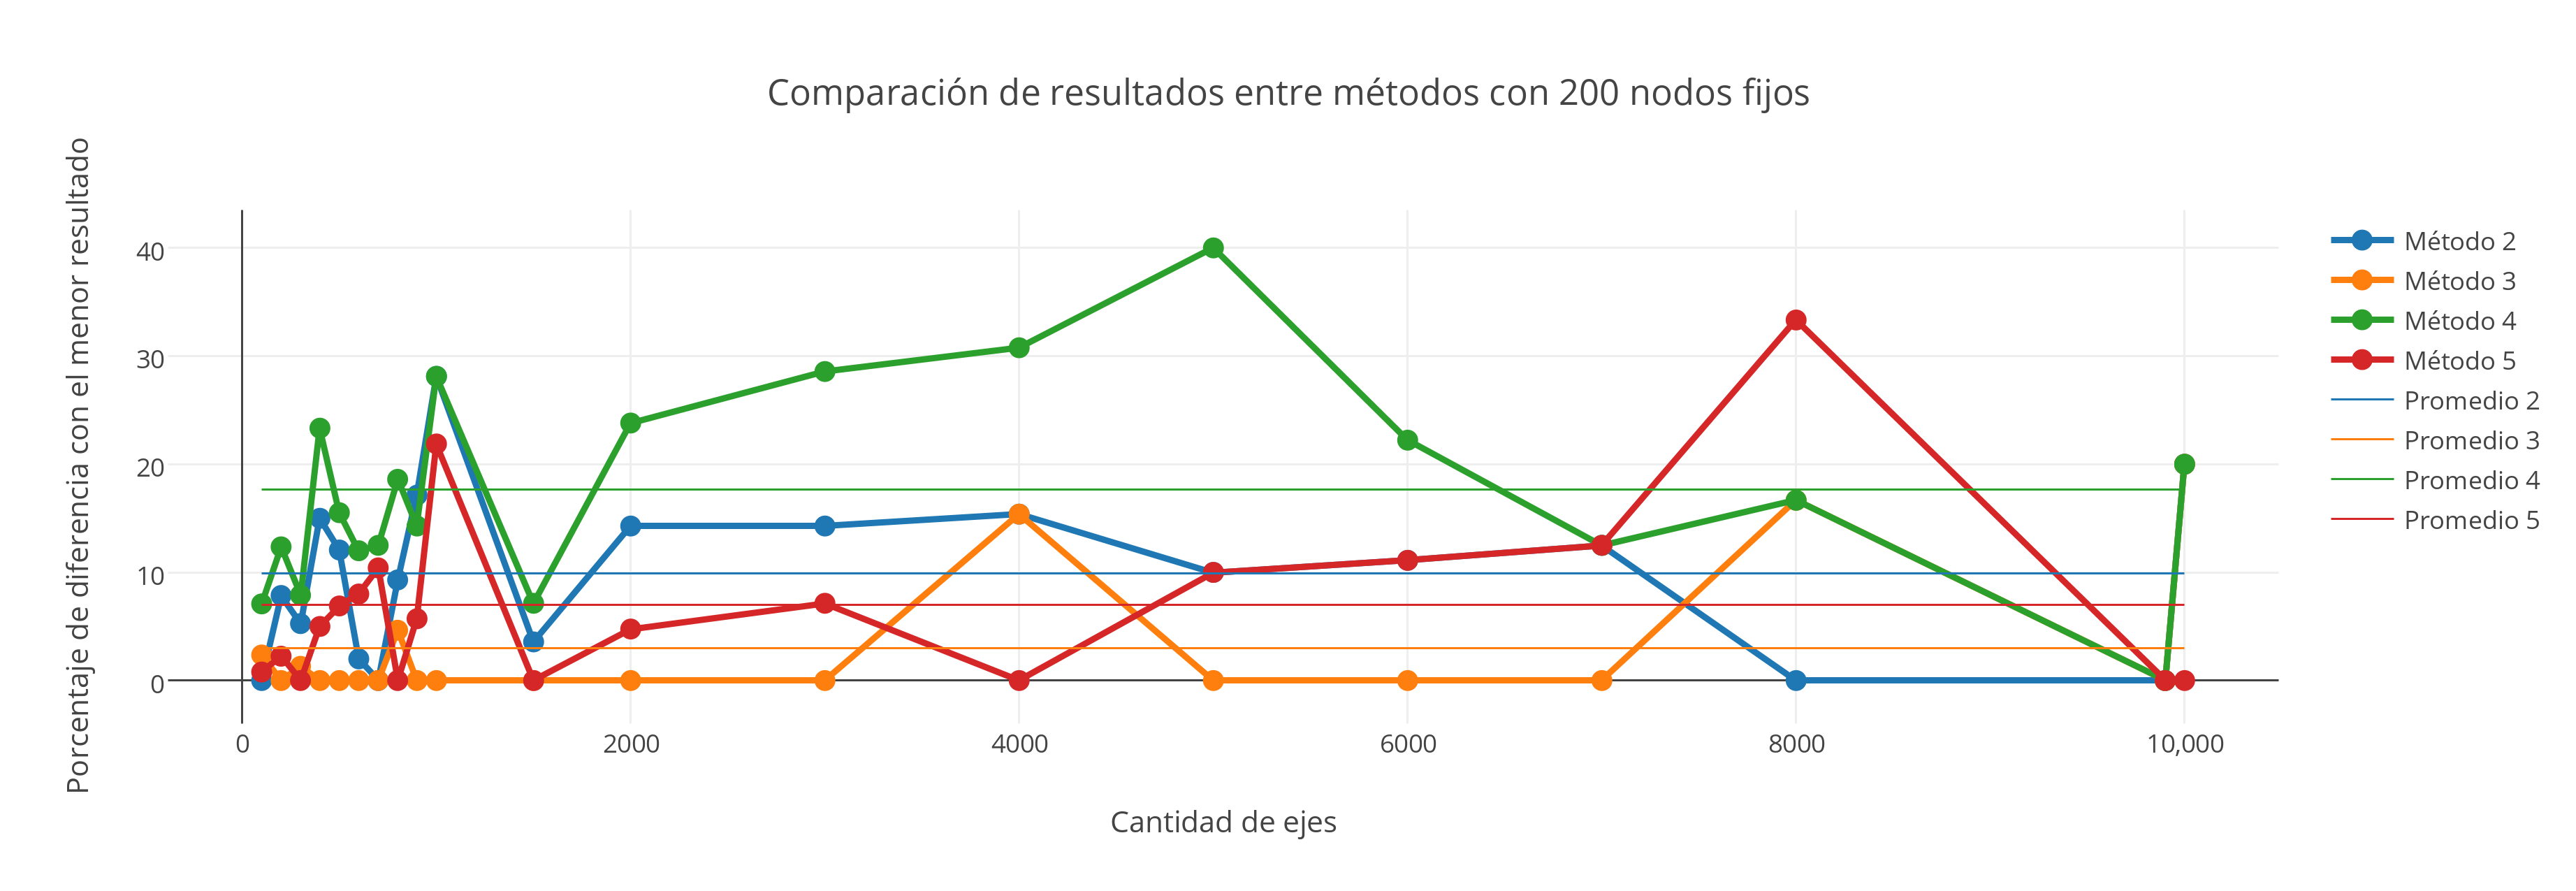
\includegraphics[scale=0.55]{imagenes/local/resultados/200nodos.png}
% 	\caption{}
%	\label{10Nodos}
   \end{center}
 \end{figure}
 
  \begin{figure}[h!]
   \begin{center}
 	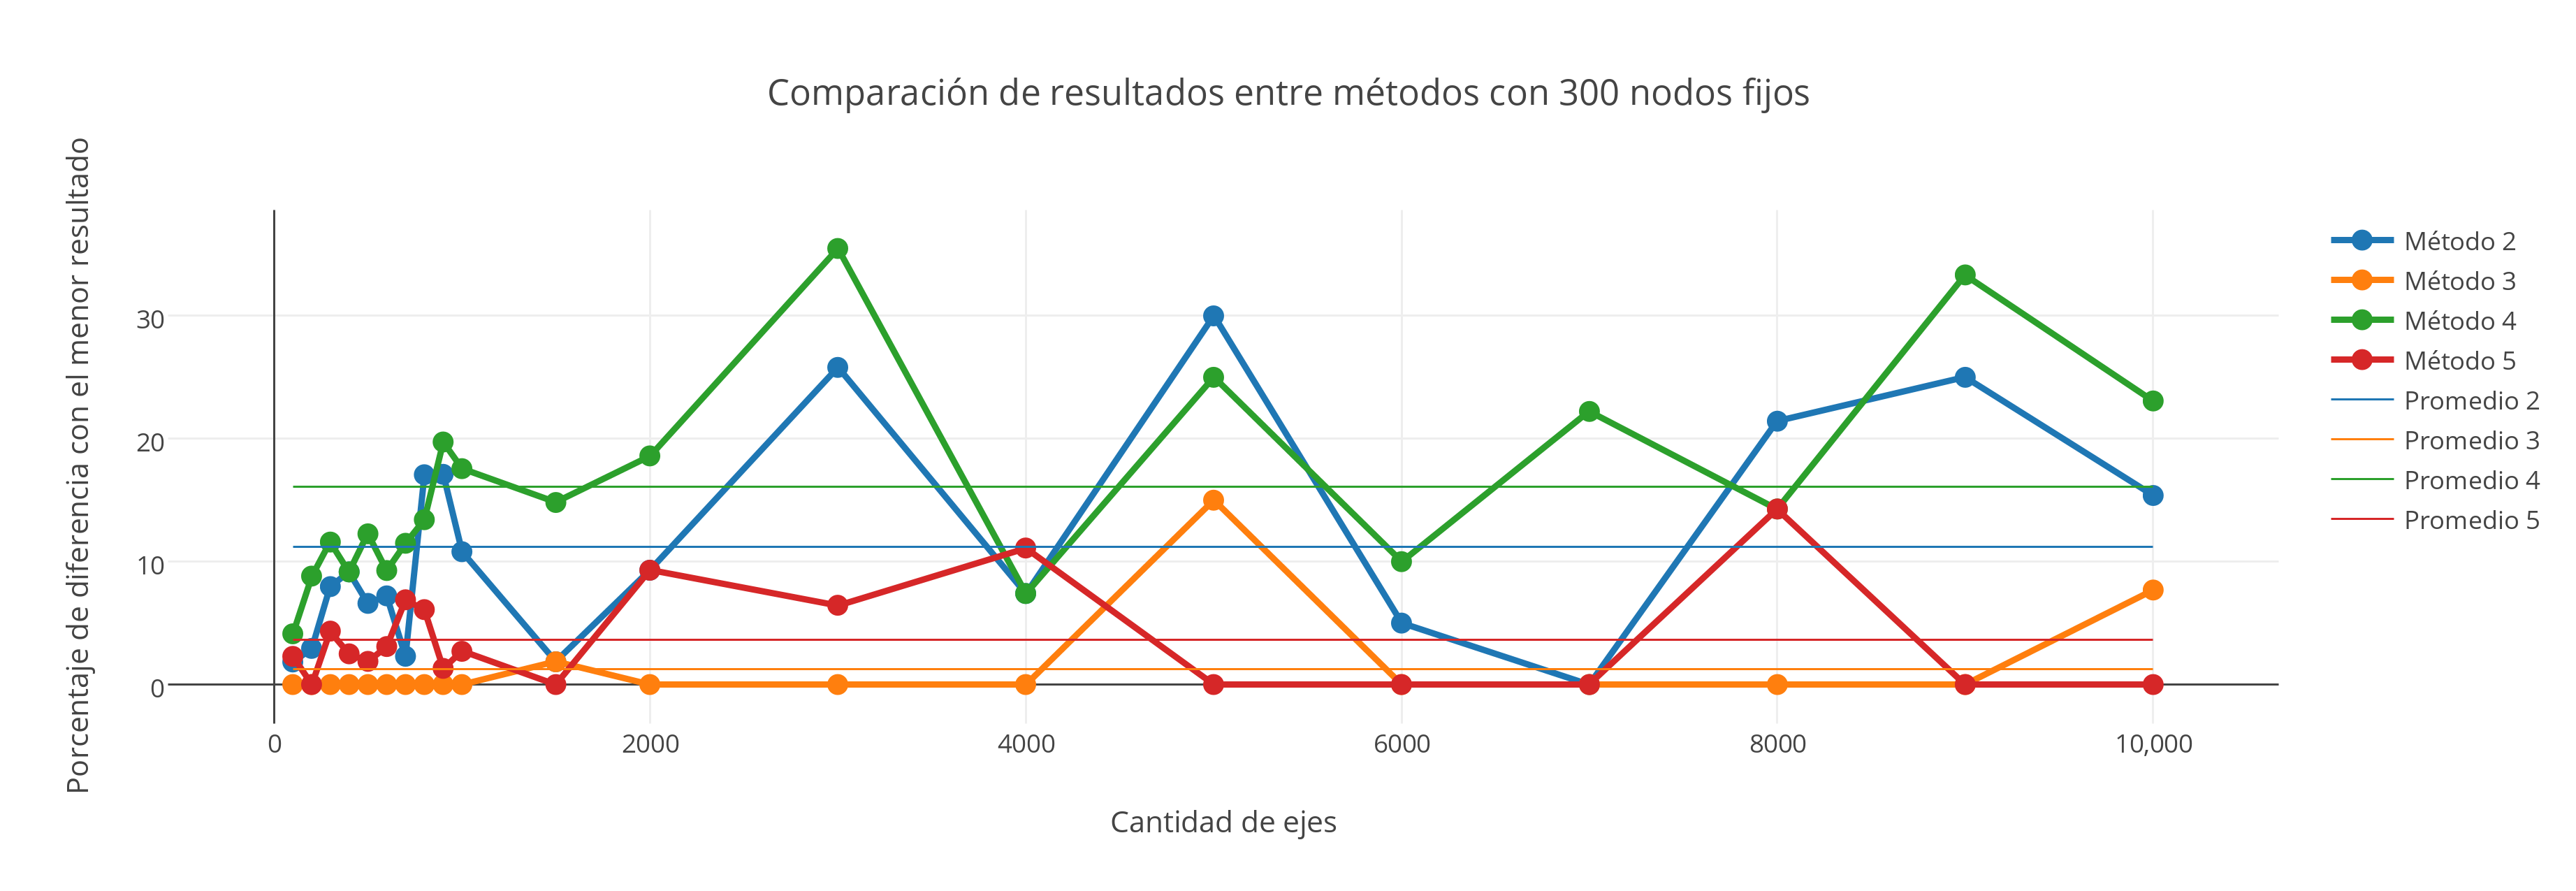
\includegraphics[scale=0.55]{imagenes/local/resultados/300nodos.png}
% 	\caption{}
%	\label{10Nodos}
   \end{center}
 \end{figure}
 

  \begin{figure}[h!]
   \begin{center}
 	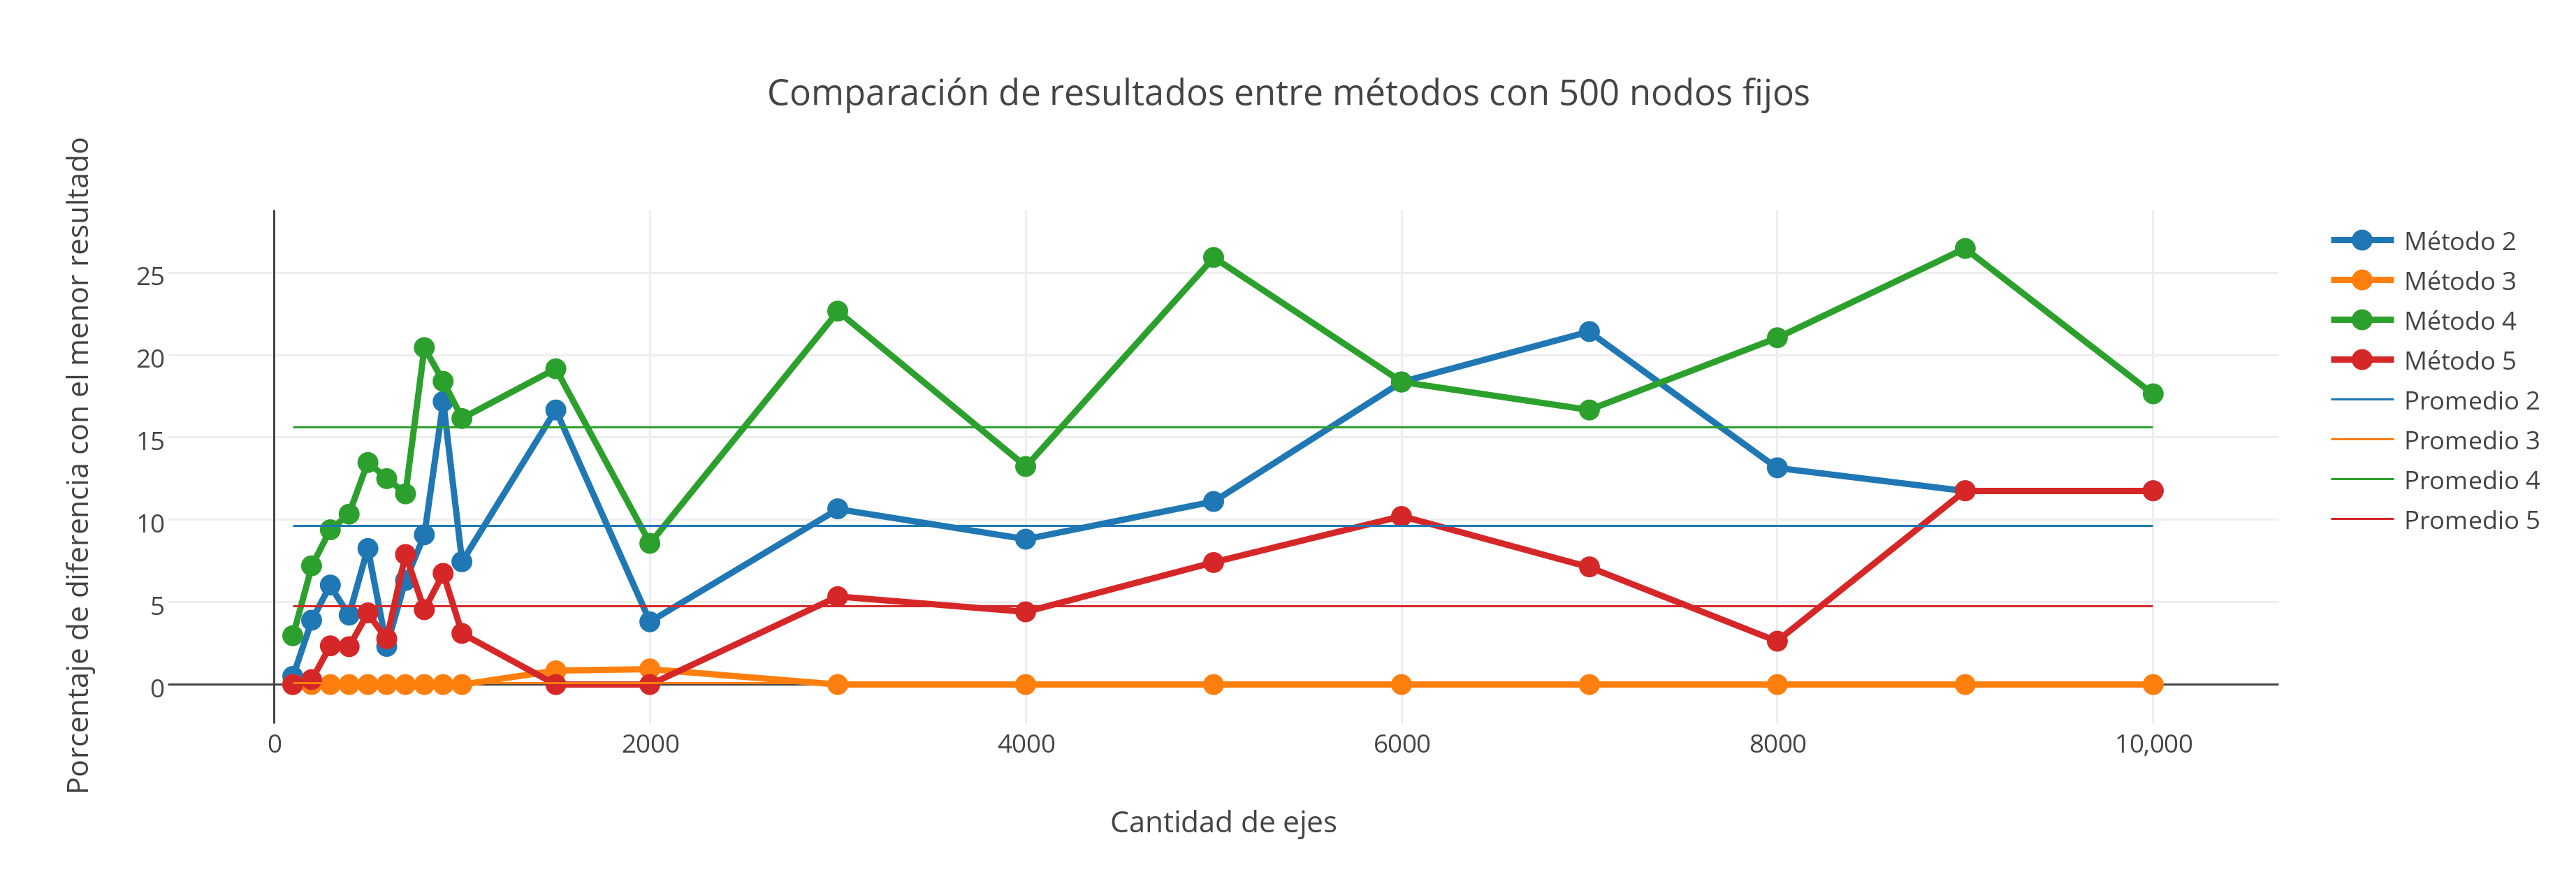
\includegraphics[scale=0.55]{imagenes/local/resultados/500nodos.png}
% 	\caption{}
%	\label{10Nodos}
   \end{center}
 \end{figure}
 
 \newpage
   \begin{figure}[h!]
   \begin{center}
 	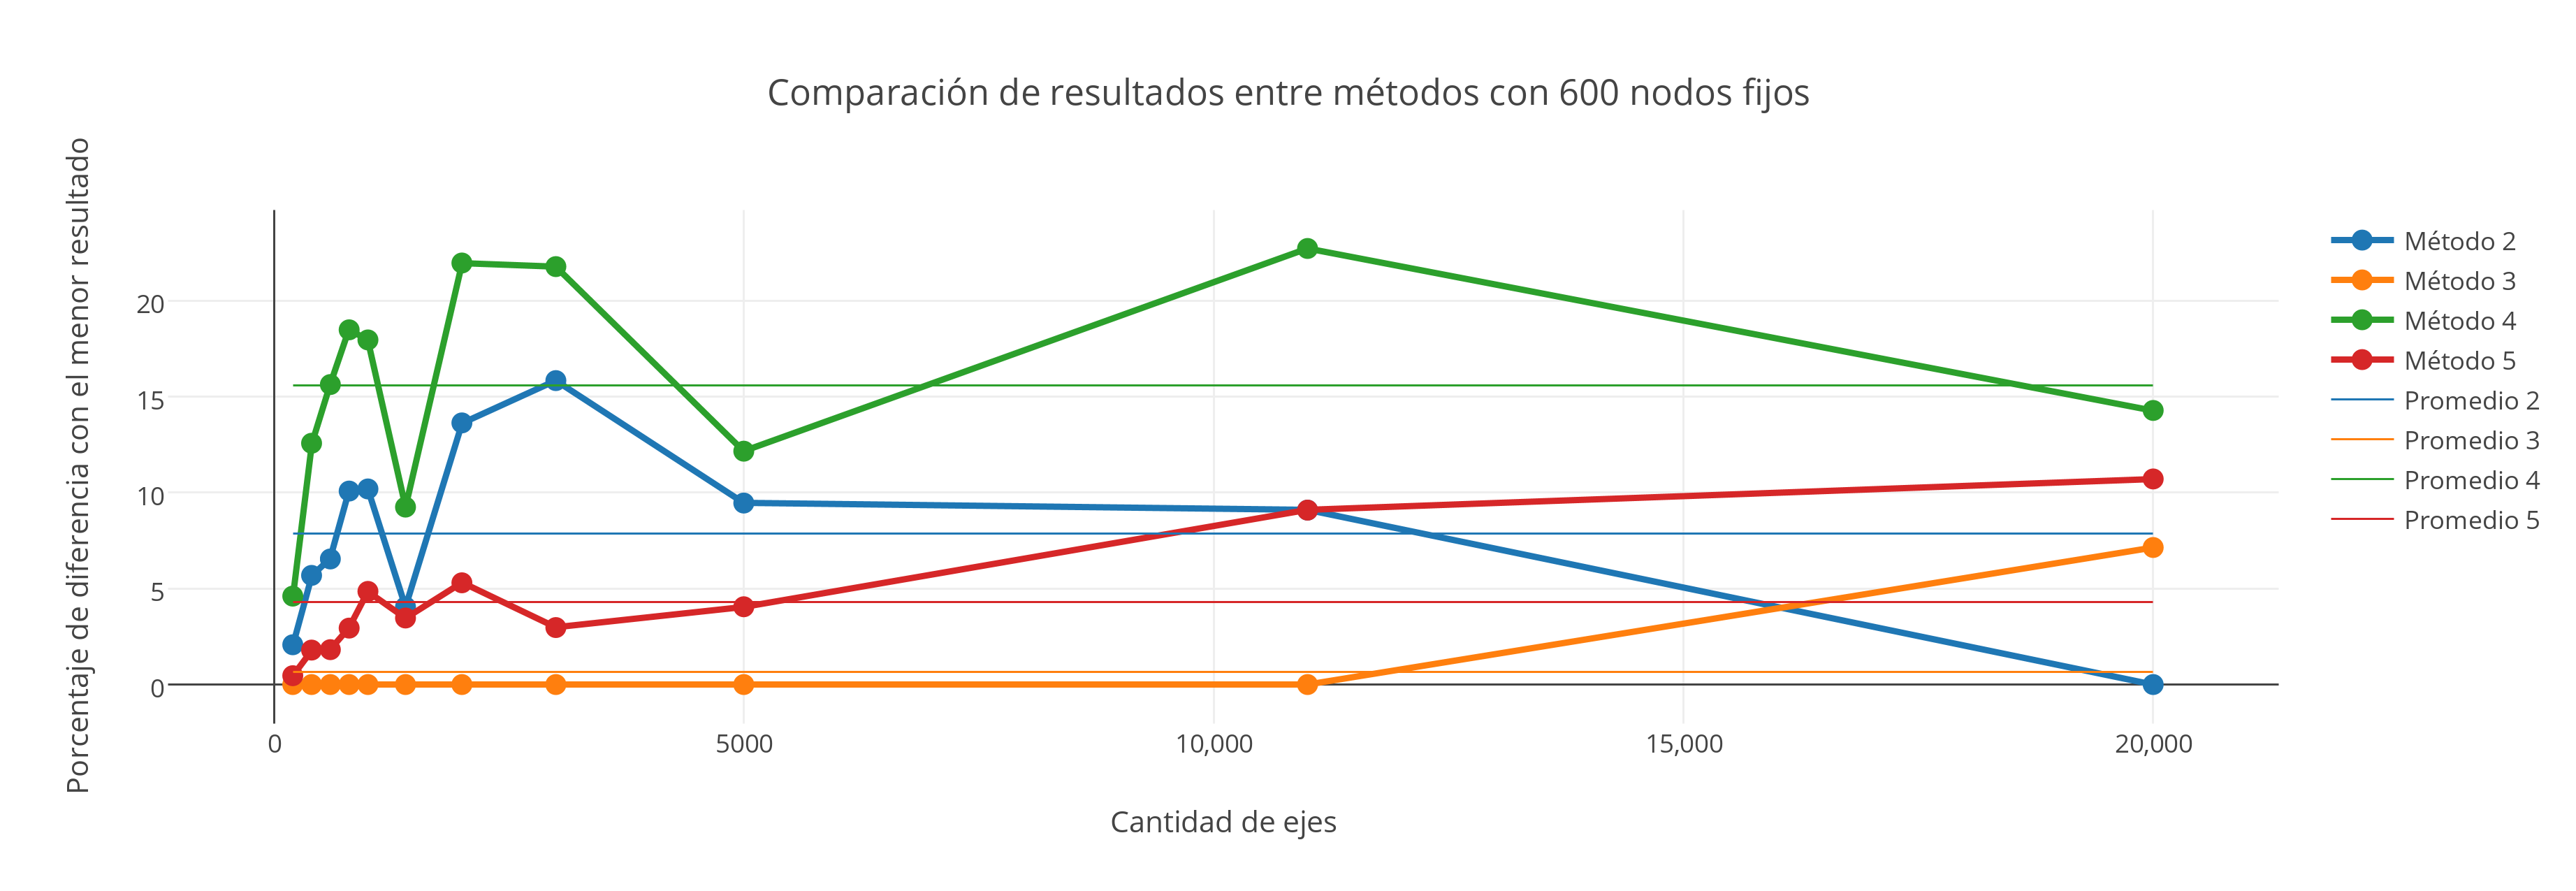
\includegraphics[scale=0.55]{imagenes/local/resultados/600nodos.png}
% 	\caption{}
%	\label{10Nodos}
   \end{center}
 \end{figure}

  \begin{figure}[h!]
   \begin{center}
 	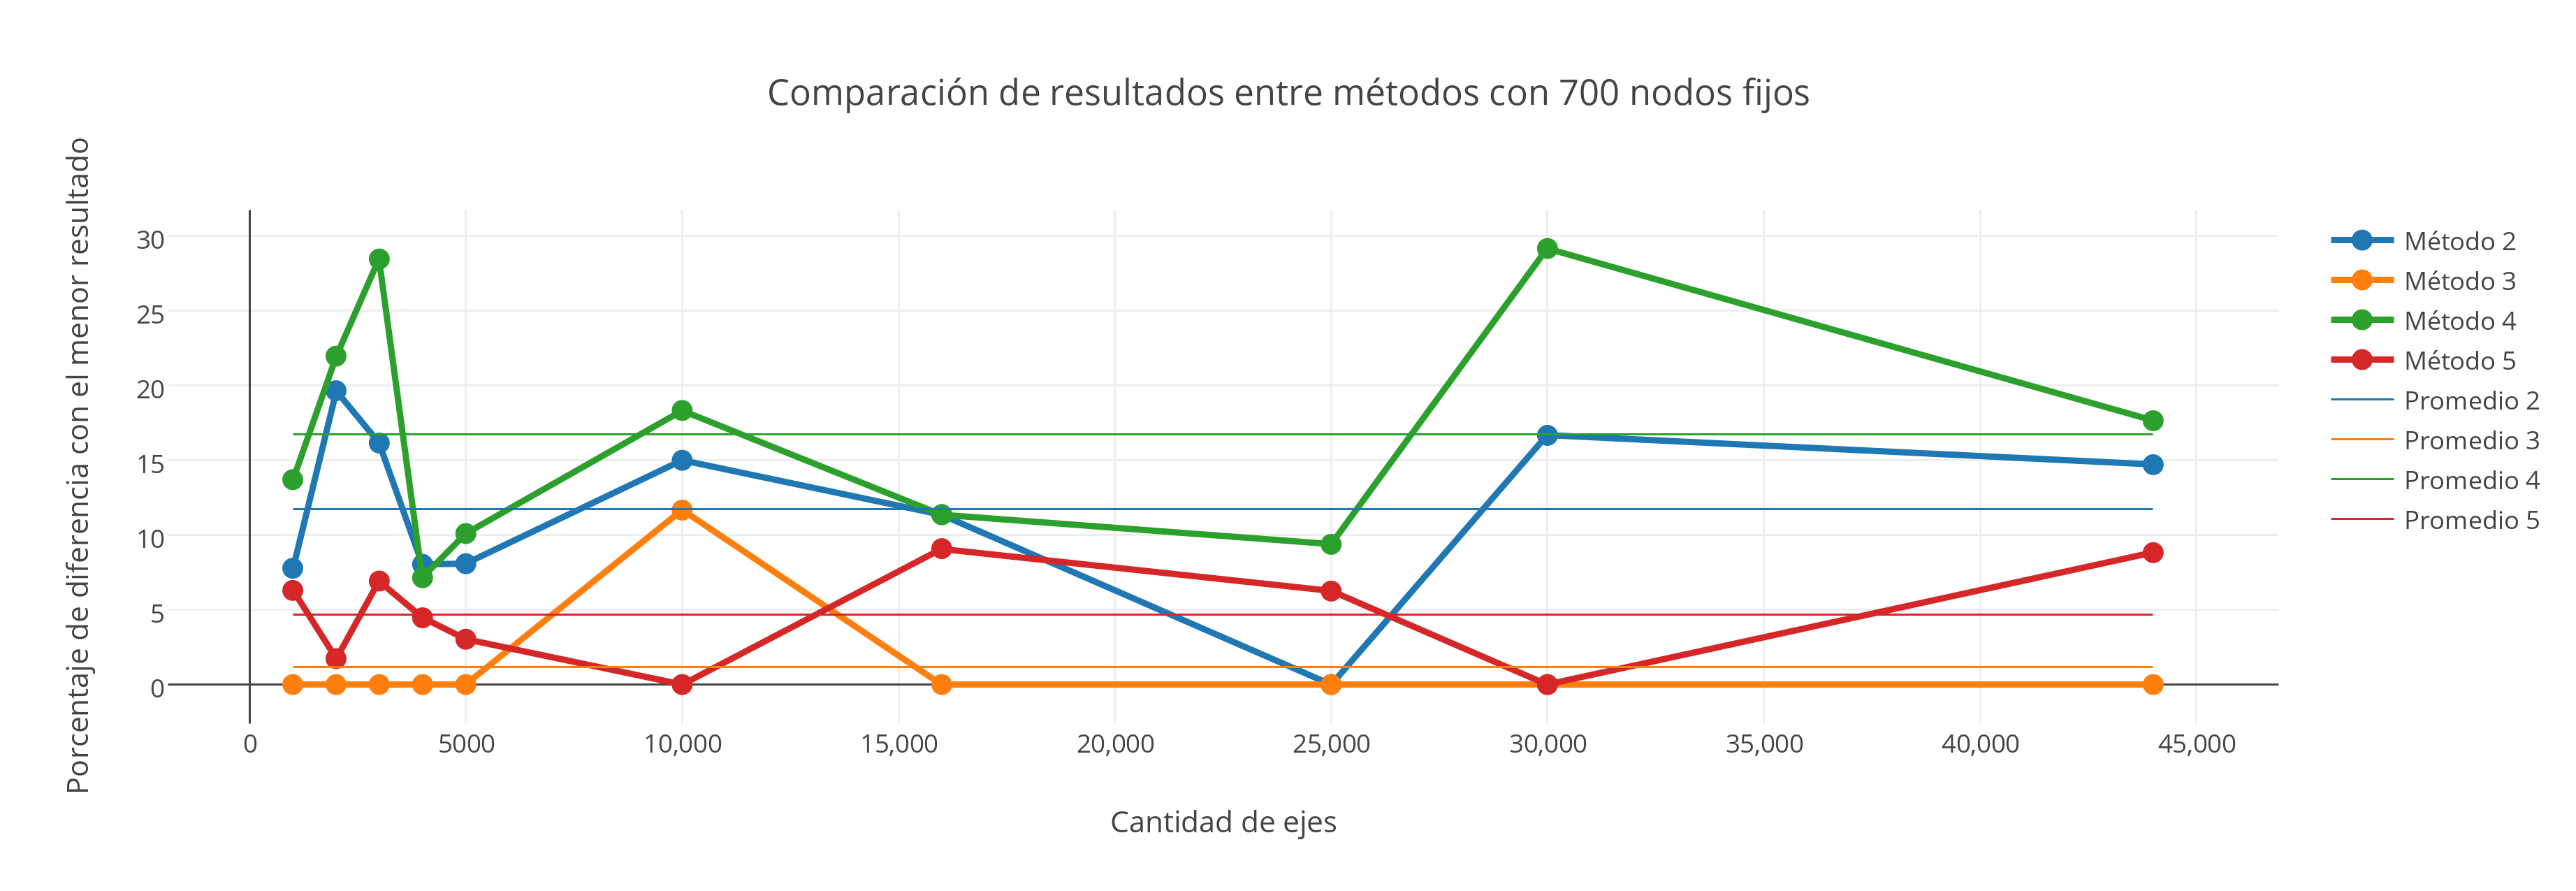
\includegraphics[scale=0.55]{imagenes/local/resultados/700nodos.png}
% 	\caption{}
%	\label{10Nodos}
   \end{center}
 \end{figure} 


\newpage